\section{EVERYTHING -- Introduction}
\label{Sec:Introduction}
% \textbf{Introduction.} ---
\note{Text printed in blue are loose notes that should not be taken too strictly.}

Astrophysical observations indicate that $85 \%$ of the total matter content in the Universe is due to dark matter (DM) \cite{Planck2015}.
Observations of stellar orbital velocities about our galactic centre give the energy density of cold (non-relativistic) DM within our local galactic neighbourhood:~$\rho_{\textrm{CDM}}^{\textrm{local}} \approx 0.4~\textrm{GeV/cm}^3$ \cite{Catena2010}, while the latest Planck satellite measurements of the cosmic microwave background (CMB) radiation give the present-day mean DM energy density:~$\bar{\rho}_{\textrm{DM}} = 1.3 \times 10^{-6}~\textrm{GeV/cm}^3$ \cite{Planck2015}.
However, the identity and physical properties of DM still remain a mystery, constituting one of the most important unsolved problems in contemporary physics.

Searches for permanent static electric dipole moments (EDMs) with neutrons \cite{Baker2006,Serebrov2014,Pendlebury2015} and atoms \cite{Griffith2009,Heckel2016} have served as the most sensitive probe to date of CP-violation in the Quantum Chromodynamics (QCD) sector \cite{Ginges2004Review,Pospelov2005Review,Engel2013Review,Roberts2015Review}.
The current limit on the $\theta_{\textrm{QCD}}$ parameter that governs CP-violation in the QCD sector, $\left|\theta_{\textrm{QCD}} \right| \lesssim 10^{-10}$, is in tension with the natural expectation that $\left| \theta_{\textrm{QCD}} \right| \sim \mathcal{O}(1)$, constituting the strong CP problem of QCD.
The most compelling and elegant resolution put forward to date for the strong CP problem is the QCD axion, which is a pseudoscalar pseudo-Nambu-Goldstone boson corresponding to the explicitly-broken global U(1)$_{\textrm{PQ}}$ symmetry \cite{PQ1977A,Weinberg1978,Wilczek1978,Kim1979,Zakharov1980,Zhitnitsky1980,Srednicki1981}.

The QCD axion and other axion-like particles (ALPs), which may arise, e.g., in string compatification models \cite{Witten1984,Conlon2006,Witten2006,Arvanitaki2010,Arias2012,Marsh2015Review}, are an excellent candidate for cold DM \cite{footnote1}.
These low-mass particles can be produced efficiently via non-thermal production mechanisms, such as vacuum misalignment \cite{Preskill1983cosmo,Sikivie1983cosmo,Dine1983cosmo}, in the early Universe, and subsequently form a coherently oscillating classical field:~$a = a_0 \cos(\omega t)$.
The angular frequency of oscillation is given by $\omega \simeq m_a c^2 / \hbar$ and the axion field carries the energy density $\rho_a \simeq m_a^2 a_0^2 /2$, where $m_a$ is the mass of the axion particle, $c$ is the speed of light and $\hbar$ is the reduced Planck constant.
Unless explicitly stated otherwise, we adopt the units $\hbar = c = 1$, with $1~\textrm{eV} = 2.4 \times 10^{14}~\textrm{Hz}$.
Although non-thermal production mechanisms typically impart negligible kinetic energy to the produced axions, the gravitational interactions between axions and ordinary matter during galactic structure formation subsequently virialise galactic axions ($v_{\textrm{vir}}^{\textrm{local}} \sim 10^{-3}c$), giving an oscillating galactic axion field the finite coherence time:~$\tau_{\textrm{coh}} \sim 2\pi / m_a v_{\textrm{vir}}^2 \sim 10^6 \cdot  2\pi / m_a $, i.e., $\Delta \omega/ \omega \sim 10^{-6}$.


It is reasonable to expect that axions interact non-gravitationally with Standard Model (SM) particles. Most types of direct searches for axions to date have focused on their coupling to photons (see, e.g., the review \cite{Axion-Review2015} and references therein). Recently, however, it has been proposed to search for the coherently oscillating spin-dependent effects due to the interactions of a coherently oscillating axion DM field with the gluons and fermions, which include anomalous spin-precession effects and CP-violating oscillating EDMs \cite{Graham2011,Flambaum2013Patras,Graham2013,Stadnik2014A,CASPEr2014,Roberts2014A}. The frequency of these oscillating effects is set by the axion mass, and importantly, these oscillating effects scale to the first power of a small interaction constant, whereas in all previously-performed axion searches, the sought effects scale to the second or fourth power of the interaction constant.


In the present work, we report on a search for ultra-low-mass axion DM by analysing the ratio of the spin-precession frequencies of stored ultracold neutrons and $^{199}$Hg atoms for an axion-induced oscillating EDM of the neutron and coupling of an oscillating galactic axion field to the nucleon spins.

\note{We may also decide to compare other clocks, in particular the Cs magnetometers with the mercury comagnetometer to obtain limits for the axion--electron coupling.}

\note{Describe the structure of the paper here.} We start with a brief theoretical overview and motivation. Our analysis is divided into two distinct parts. Firstly, we present an analysis of the Sussex--RAL--ILL nEDM experiment data, to which we shall refer as the \emph{long time--base} or \emph{run--level} analysis. \note{MR: We may want to simplify the nomenclature.} Then we present how this analysis has been extended to analyse the PSI nEDM experimental data on a \emph{short time--base} or \emph{cycle--level}. Lastly, we present the results of both analyses in the landscape of already available limits.


%%%%%%%%%%
\section{Theory}
% \textbf{Theory.} ---
The relevant couplings of the axion to the SM fields are:
\begin{align}
\label{Axion_couplings}
\mathcal{L}_{\textrm{int}} = \frac{C_G}{f_a} \frac{g^2}{32\pi^2} a G^{a}_{\mu \nu} \tilde{G}^{a \mu \nu}  ~ - \sum_{f=n,p,e} \frac{C_f}{2f_a} \partial_\mu a ~ \bar{f} \gamma^\mu \gamma^5 f \, .
\end{align}
The first term represents the coupling of the axion field to the gluonic field tensor $G$ and its dual $\tilde{G}$, with summation over the colour index $a=1,2,...,8$, $g^2 / 4 \pi$ is the colour coupling constant and $f_a$ is the axion decay constant. The second term represents the coupling of the derivative of the axion field to the nucleon axial-vector currents $\bar{N} \gamma^\mu \gamma^5 N$ and to the electron axial-vector current $\bar{e} \gamma^\mu \gamma^5 e$.
$C_G$ and $C_f$ are model-dependent dimensionless parameters.

There is strong motivation from cosmology to explore axion DM in the mass range $10^{-22}\text{ eV}\lesssim m_a \lesssim 10^{-12}\text{ eV}$ for $10^{10}\text{ GeV}\lesssim f_a \lesssim 10^{18}\text{ GeV}$.
The axion couplings in Eq.~(\ref{Axion_couplings}) for these parameter values are relatively unconstrained.
The existing constraints on the axion mass and interaction parameters in Eq.~(\ref{Axion_couplings}) from laboratory searches and measurements pertaining to astrophysics and cosmology are summarised in Appendix A.
A model for ultra-low-mass axions with $m_af_a\ll \Lambda_{\mathrm{QCD}}^2$, and simultaneously $C_G\sim 1$, is presented in Appendix B.

The first term in Eq.~(\ref{Axion_couplings}) induces the following oscillating EDM of the neutron via the process in Fig.~1a \cite{Graham2011,Stadnik2014A,Witten1979,Pospelov1999}:
\begin{align}
\label{nEDM_axion}
&d_n(t) \approx 2.4 \times 10^{-16} ~ \frac{C_G a_0}{f_a} \cos(m_a t) ~ e \cdot \textrm{cm} \notag \\
&\approx 2.4 \times 10^{-16} ~ \frac{C_G \sqrt{2 \rho_{\textrm{CDM}}^{\textrm{local}} \Omega_a / \Omega_{\textrm{CDM}}}}{m_a f_a} \cos(m_a t) ~  e \cdot \textrm{cm} \notag \\
&\approx 5.9 \times 10^{-22} C_G \left( \frac{10^{-22} \textrm{eV}}{m_a} \right) \left( \frac{10^{16} \textrm{GeV}}{f_a} \right)  \cos(m_a t) ~ e \cdot \textrm{cm} \, ,
\end{align}
where we have made use of the relation $\rho_a \simeq m_a^2 a_0^2 /2$ and where $\Omega_a / \Omega_{\textrm{CDM}}$ is the relative contribution of axions to the local cold DM energy density ($\rho_{\textrm{CDM}}^{\textrm{local}} \approx 0.4~\textrm{GeV/cm}^3$ \cite{Catena2010}), which we have assumed to be unity in the last line \cite{footnote2,footnote3}.
The first term in Eq.~(\ref{Axion_couplings}) induces the following oscillating EDM of the $^{199}$Hg atom via the intrinsic oscillating nucleon EDMs (Fig.~1a) and oscillating P,T-violating intranuclear forces (which is the dominant contribution, Fig.~1b) \cite{Stadnik2014A,Flambaum1984EDM,Flambaum1985EDM,Flambaum2002EDM,Dmitriev2003A,Dmitriev2005,Engel2005,Engel2010}:
\begin{align}
\label{199Hg-EDM_axion}
&d_{\textrm{Hg}}(t) \approx -1.8 \times 10^{-19} ~ \frac{C_G a_0}{f_a} \cos(m_a t) ~ e \cdot \textrm{cm} \notag \\
&\approx -1.8 \times 10^{-19} ~ \frac{C_G \sqrt{2 \rho_{\textrm{CDM}}^{\textrm{local}} \Omega_a / \Omega_{\textrm{CDM}}}}{m_a f_a} \cos(m_a t) ~ e \cdot \textrm{cm} \notag \\
&\approx -4.5 \times 10^{-25} C_G \left( \frac{10^{-22} \textrm{eV}}{m_a} \right) \left( \frac{10^{16} \textrm{GeV}}{f_a} \right)  \cos(m_a t) ~ e \cdot \textrm{cm} \, .
\end{align}
%where we have again made use of the relation $\rho_a \simeq m_a^2 a_0^2 /2$ and have assumed $\Omega_a / \Omega_{\textrm{CDM}} = 1$ in the last line.
The temporal component of the axion-electron coupling in Eq.~(1) also produces an oscillating atomic EDM \cite{Stadnik2014A,Roberts2014A}, though this mechanism is suppressed in diamagnetic atoms with zero electron angular momentum, such as the $^{199}$Hg atom.


\begin{figure}[h!]
  \begin{center}
  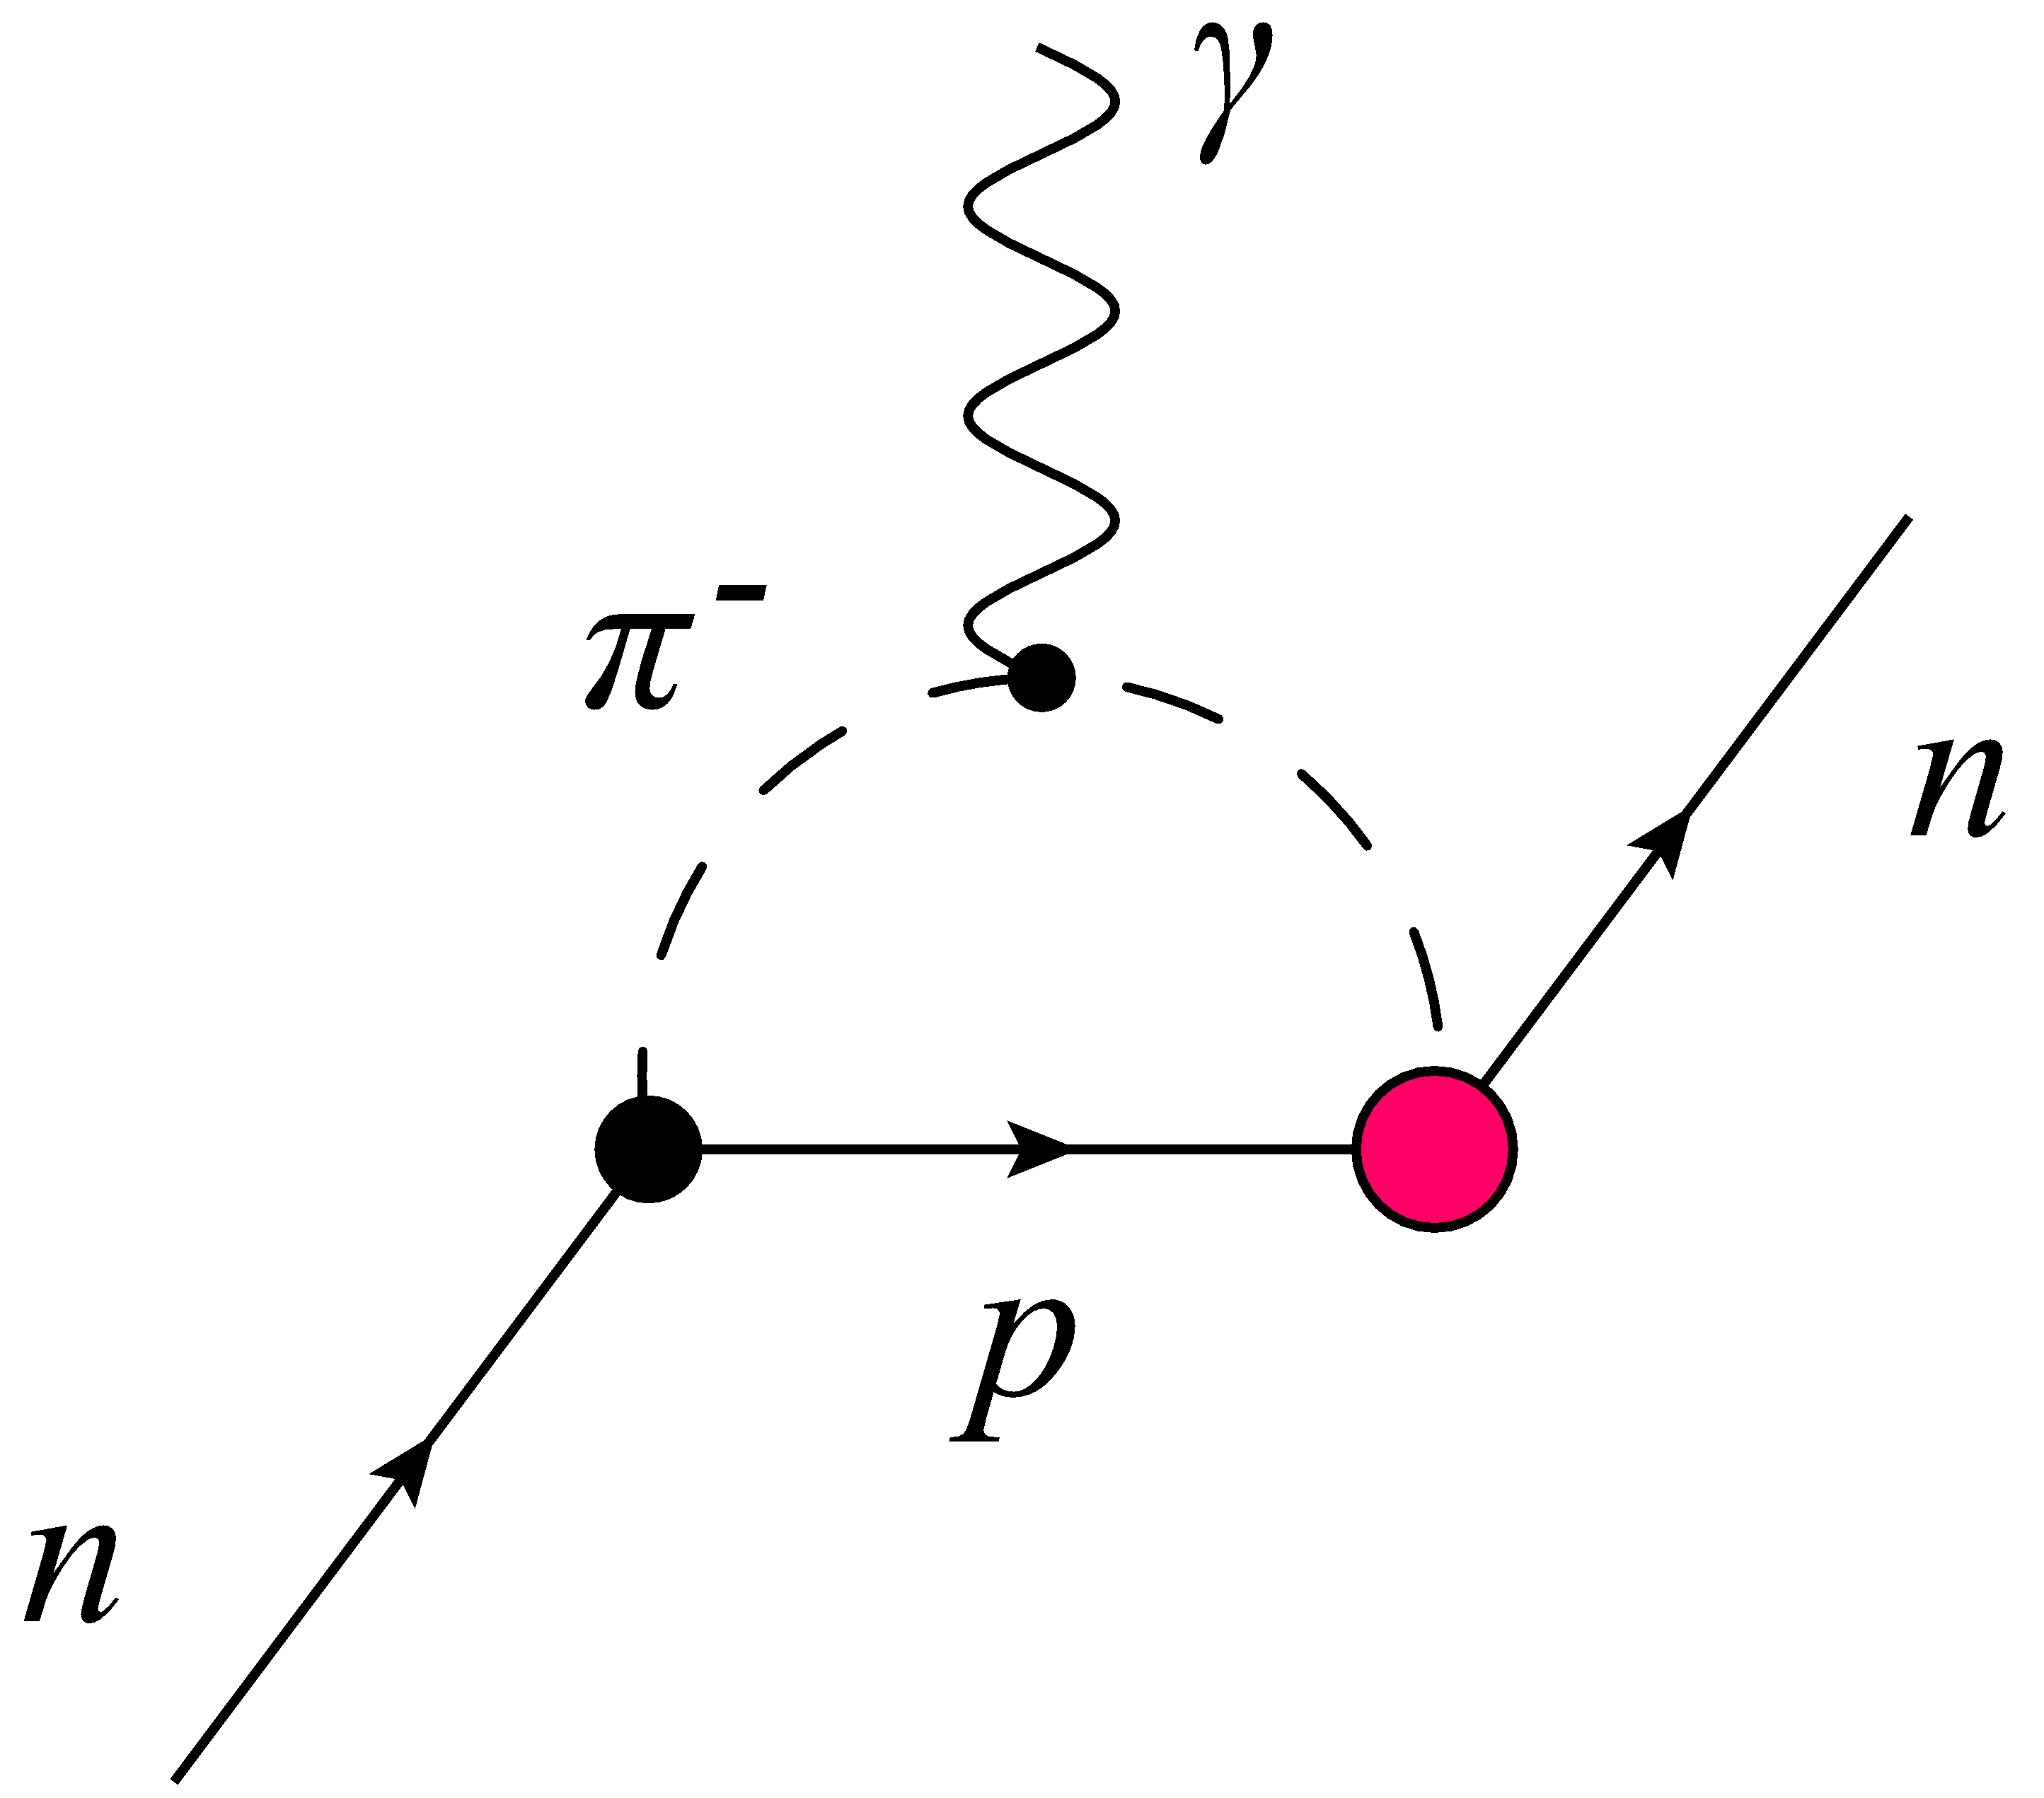
\includegraphics[width=3.3cm]{gfx/axions/nEDM_soft_pion_limit_NEW.png}
  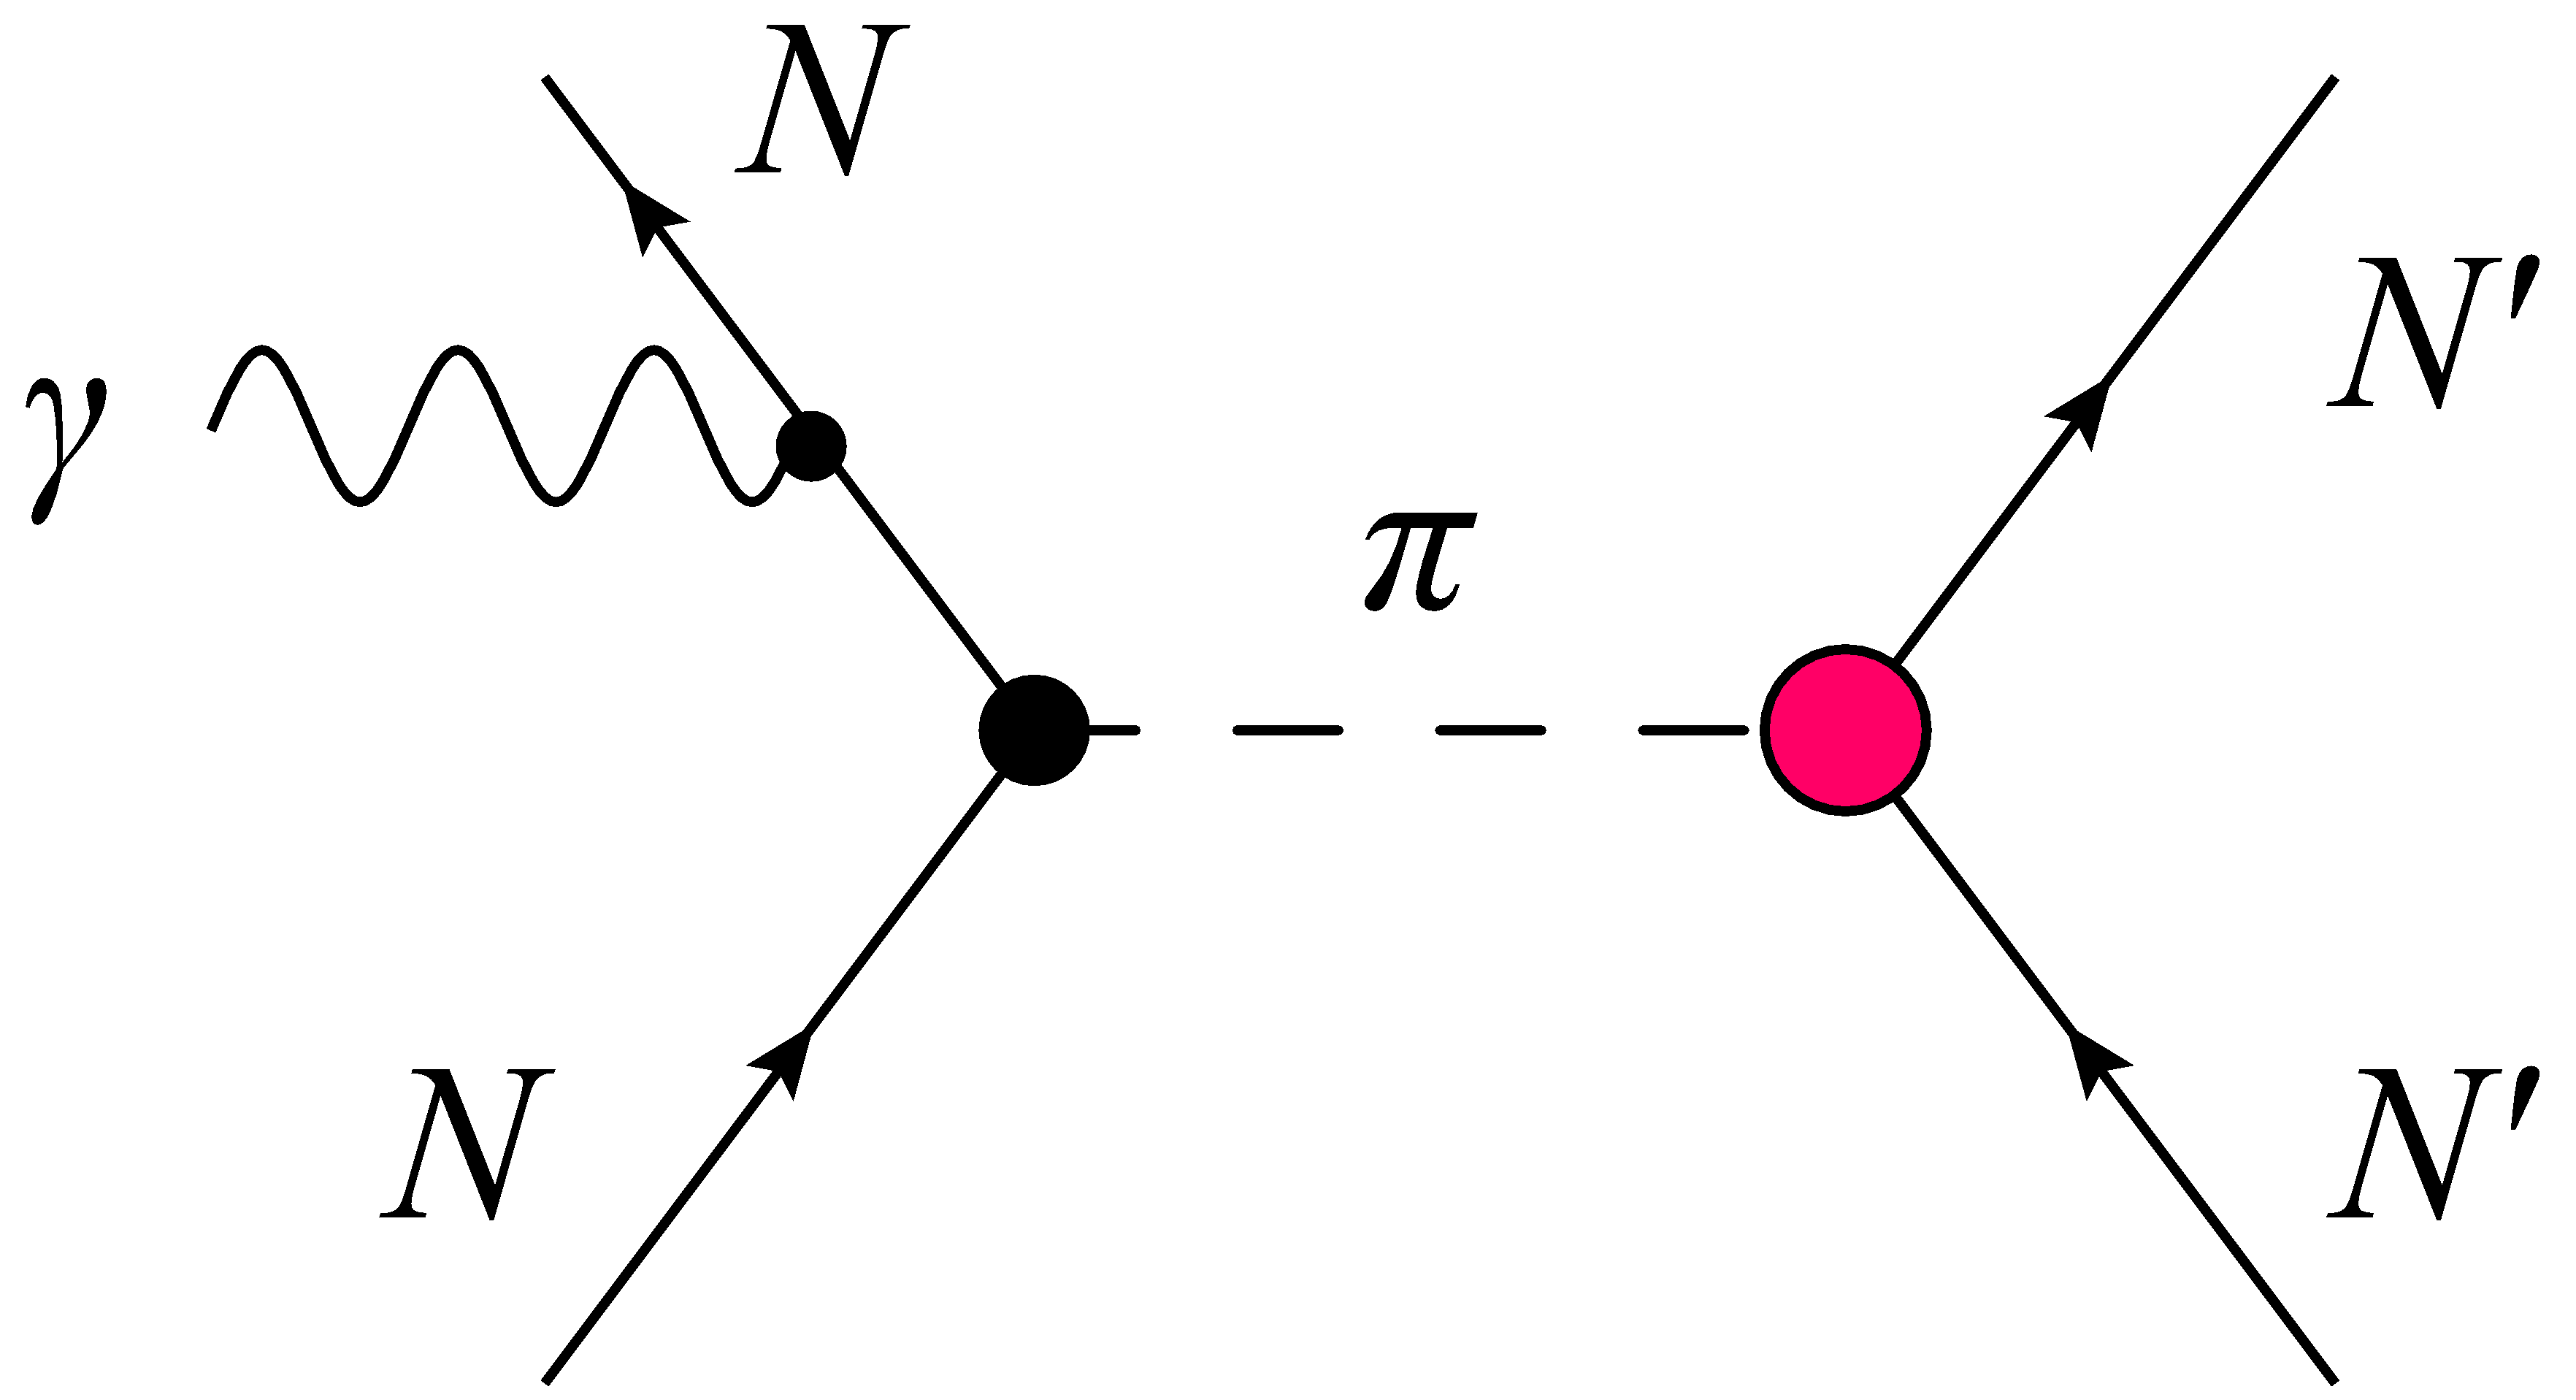
\includegraphics[width=4.1cm]{gfx/axions/Pion_nucleon_PT-odd_NEW.png}
  \caption{(Color online) Fig.~1a: Process responsible for axion-induced oscillating EDMs of the free neutron and of nucleons (replace the $\pi^{-} p$ loop by a $\pi^{+} n$ loop for the proton) in atomic nuclei.
  Fig.~1b: Dominant process for axion-induced oscillating P,T-violating electromagnetic moments of atomic nuclei.
  Bold black circles denote the usual P,T-conserving $- i g_{\pi N N}  \bar{N}  \gamma^5 \tau^b N \pi^b$ vertex, while magenta circles denote the axion-induced P,T-violating $\bar{g}_{\pi N N}^{(0)} \bar{N} \tau^b N \pi^b$ vertex, with $g_{\pi NN} = 13.5$, $\bar{g}_{\pi N N}^{(0)} \approx 0.027 a_0/f_a \cos(m_a t)$ \cite{Witten1979} (a more recent value calculated from SU(3) chiral perturbation theory gives $\bar{g}_{\pi N N}^{(0)} =0.016 a_0/f_a \cos(m_a t)$ \cite{Mereghetti2015}), and where the sums run over the isospin index $b=1,2,3$.  }
  \end{center}
\end{figure}


An oscillating galactic axion field, $a = a_0 \cos(m_a t - \vtr{p}_a \cdot \vtr{r})$, produces the following time-dependent non-relativistic potential for a spin-polarised source, via the spatial components of the second term in Eq.~(\ref{Axion_couplings}):
\begin{equation}
\label{potential_axion-wind}
H_{\textrm{int}} (t) \simeq \sum_{f=n,p,e} \frac{C_f \sqrt{\rho_{\textrm{CDM}}^{\textrm{local}} \Omega_a / \Omega_{\textrm{CDM}}}}{\sqrt{2} m_a f_a} \sin(m_a t) ~ \vtr{\sigma}_f \cdot \vtr{p}_a \, ,
\end{equation}
where we have made use of the relation $\rho_a \simeq m_a^2 a_0^2 /2$, and $\vtr{p}_a = m_a \vtr{v}_a$ is the average axion momentum relative to the Solar System ($|\vtr{v}_a| \sim 10^{-3} c$).
We evaluate the term $\vtr{\sigma}_f \cdot \vtr{p}_a$ in Eq.~(\ref{potential_axion-wind}) by transforming to a non-rotating celestial coordinate system (see, e.g., \cite{Kostelecky1999}) \note{MR: This transformation assumes a particular choice of $t=0$, as stated in Sec.\,IID of \cite{Kostelecky1999}}:
\begin{align}
\label{sigma-p_a_2}
\vtr{\sigma}_f \cdot \vtr{p}_a & = \hat{m}_F f(\sigma_f) m_a |\vtr{v}_a|  \notag \\
&\times \left[\cos(\chi) \sin(\delta) + \sin(\chi) \cos(\delta) \cos(\Omega_{\textrm{sid}} t - \eta) \right] \, ,
\end{align}
where $\chi$ is the angle between Earth's axis of rotation and the spin quantisation axis ($\chi = 44.8^\circ$ at Grenoble), $\delta \simeq -48 ^\circ$ and $\eta \simeq 138 ^\circ$ are the declination and right ascension, respectively, of the galactic DM flux relative to the Solar System \cite{NASA2014web}, $\Omega_{\textrm{sid}} = 2\pi / (23.93~\textrm{hours})$ is the daily sidereal angular frequency, $\hat{m}_F = m_F / F$, with $F$ being the total angular momentum and $m_F$ being the projection of $F$ onto the quantisation axis, and $f(\sigma_f)$ is the fermion spin-content function (see Table \ref{tab:spin-content-function-values} for the relevant values).
%\note{Notes for later: Sagnac effect and gyroscopic shift due to Earth's rotation; stability of direction of spin polarisation?}


%%%%
  \begin{table}[h!]
    \centering%
    \caption{Calculated values of the fermion spin-content function for the free neutron, $^{199}$Hg atom and $^{133}$Cs atom. We have used the calculated neutron and proton spin contributions for the $^{199}$Hg and $^{133}$Cs nuclei from \cite{Stadnik2015NMBE}.}
%\begin{tabular}%
\begin{tabular}{cccc}
\multicolumn{1}{c}{Species}   & \multicolumn{1}{c}{$f(\sigma_n) $}   & \multicolumn{1}{c}{$f(\sigma_p) $} & \multicolumn{1}{c}{$f(\sigma_e) $ }   \\
\hline
free neutron	&	1	&	0	&	0	\\
$^{199}$Hg atom	&	$-$0.30	&	$-$0.03	&	0	\\
$^{133}$Cs atom ($F=4$ state)	&	$-$0.21	&	$-$0.57	&	1	\\
$^{133}$Cs atom ($F=3$ state)	&	$-$0.20	&	$-$0.55	&	$-$0.75	\\
  \end{tabular}%
%\end{tabular}%
    \label{tab:spin-content-function-values}%
  \end{table}%.
%%%%%%%%%%







%%%%%%%%%%%%%%%%
\section{Long time--base analysis}
% \textbf{Experiment.} ---

\note{Description of experiment and analysis.}

\note{Point out that ultracold neutrons have previously been used as a sensitive probe in searches for a permanent static EDM of the neutron \cite{Baker2006,Serebrov2014,Pendlebury2015}, and for a gravitational dipole moment of the neutron, and tests of the invariance of the Lorentz and CPT symmetries \cite{Altarev2009,Altarev2010}.}

\subsection{The Sussex-RAL-ILL Room Temperature Neutron Electric Dipole Moment Experiment}
\note{NA: this subsection is still a very early draft, I know there are still formatting issues and blanks}

\note{This first bit is paraphrased from C.A. Baker et al., Apparatus for Measurement of the Electric Dipole Moment of the Neutron using a Cohabiting Atomic-Mercury Magnetometer}

\note{MR: This should probably be made much shorter.}

Most experiments to measure the static electric dipole moment of the neutron use magnetic resonance techniques to observe the Larmor precession of free neutrons in parallel and antiparallel magnetic and electric fields. The Hamiltonian of an uncharged spin $1/2$ particle in an electric and a magnetic field is:
\begin{equation}
H = - 2\vec{S} \cdot (\mu \vec{B} + d \vec{E})
\end{equation}
In the case of parallel and antiparallel magnetic and electric fields, this gives a precession frequency of:
\begin{equation}
h\nu = -2\mu B \mp 2dE
\end{equation}
In the presence of a non-zero EDM, when the direction of the applied electric field is reversed relative to the magnetic field we expect a shift in the precession frequency of
\begin{equation}
\delta \nu _0 = −\frac{4d_n E_0}{h} .
\end{equation}
In the Sussex-RAL-ILL Room Temperature experiment, polarised ultracold neutrons produced at the fundamental physics beamline at the ILL high flux reactor were stored in a material bottle (a cylinder of diameter 235mm and height 120mm), wherein their precession frequency in parallel and antiparallel combinations of electric and magnetic fields was measured using the Ramsey Technique. To combat drifts in the magnitude of the applied magnetic field, a cohabiting magnetometer of atomic $^{199}$Hg was used, and analysis was done by considering the ratio of neutron and mercury precession frequencies, “$R$”.

Each measurement sequence (“cycle”) consisted of a filling period, a first $\pi/2$ pulse to rotate the neutron spins into the horizontal plane, a 130s period of free precession, a second $\pi/2$ pulse to project the spins onto the z axis, and an emptying period where the number of spin-up and spin-down neutrons were counted. The precession of the mercury during the free precession period was measured by observing the modulation of the absorption of light from a mercury discharge lamp \note{is it actually a discharge lamp?}. Each cycle lasted in total x minutes. Many cycles were taken at each fixed magnetic field configuration over the course of between 1 and 73 hours (a “run”), while the direction of the applied electric field was reversed every 20 cycles. From each run a value of the neutron to mercury frequency ratio $R$ was extracted, as well as a value of the apparent EDM.

As a result of a conspiracy between radial magnetic field components and rotating magnetic components arising from the Lorentz transformation of the large applied electric field into the rest frame of the mercury atoms, a frequency shift proportional to the applied electric field was observed, mimicking the effect of a non-zero electric dipole moment of the neutron --- a “false EDM”. This effect is, however, directly proportional to the gradient of the applied vertical magnetic field dBz/dz, and reverses with the sign of the applied magnetic field. The false EDM effect has been analysed in more detail in \note{cite false edm paper(s)} and a direct measurement of this effect was made in \note{cite false edm measurement}.

As the ILL experiment had no direct measurement of the vertical gradient, the measurement of the neutron to mercury frequency ratio was instead used as a proxy. Due to the extremely low energy of the ultracold neutron population, the centre of mass of the neutron population sags a little below the centre of the precession chamber. The relatively hot population of mercury atoms does not suffer from this effect, so there is an effective height difference $\Delta h \approx 3.7 \mathrm{mm}$ between the neutron and mercury populations. Thus, the ratio of neutron to mercury frequencies depends (to first order) on the vertical gradient like: \note{MR: We might want to get rid of the stacked fraction for clarity.}
\begin{equation}
  R = R_0 \left( 1 + \Delta h  \frac{\frac{\mathrm{d}B_z}{\mathrm{d}z}}{B_{0}} \right).
  \label{eq:R}
\end{equation}
This frequency shift does not uniformly affect the entire neutron population: the effect is much greater for the lowest energy neutrons which have a lower centre of mass. This causes a departure from the linear relation above; however, in the low vertical gradient regime ($\lesssim 30 \mathrm{pT/cm}$) in which most of the data was taken, the effect is almost exactly linear. This effect is described more thoroughly in [cite grav depol papers].

To correct for these false EDMs in static EDM searches, the “crossing lines” procedure was adopted.  For each direction of the magnetic field, the measured EDM value was plotted against the measured neutron to mercury frequency ratio. Barring other systematic shifts, it is considered that the vertical gradient is zero where these lines cross. Other effects arising from transverse magnetic fields, the rotation of the earth and cause additional frequency shifts in the neutrons or in the cohabiting magnetometer, which can \note{PH: no it isn't -- there are still systematics from e.g. transverse fields, which can move the crossing point away from dB/dz=0, in addition to effects such as Earth's rotation that result in a vertical shift of the crossing point...]}, and therefore a measurement of the neutron electric dipole moment independent of the false EDM effect and of the neutron to mercury frequency ratio independent of the gravitational shift can be extracted. In the rest of the run-level analysis, we work with data where these false EDM effects have been subtracted. Further systematic effects shift the measured neutron to mercury frequency ratio or the measured EDM value, however these effects can be assumed to have been constant throughout the entire experimental measurement period, and so will not be further explored in this analysis. Systematic effects affecting the static analysis of the ILL experiment are explored in depth in [cite reanalysis] and [cite apparatus paper].

\note{MR: Need to mention explicitly, that the average $d_n$ over a run is measured (though not exactly, it is only over the free precession periods), and this is how it is treated in the Monte Carlo simulations.}

% \subsection{Analysis strategy}
% We are looking for oscillations in the neutron EDM value $d_n$. Our analysis is split into two distinct parts. Firstly, we perform a Run--Level analysis using the Sussex--RAL--ILL data. There we are looking for time series...
% MR: moved to the introduction

\subsection{Least Squares Spectral Analysis}
In this section, we present the statistical methods we use. We start by defining the \emph{periodogram}, which serves as a transition from time to the frequency space, natural for looking for oscillations. Next we proceed to discuss the statistical properties of the periodogram, which lays the basis for this analysis.

A \emph{periodogram} is an estimator of the power spectrum. With the Least Squares Spectral Analysis (LSSA) method one can construct a statistically well--behaving periodogram for non-uniformly sampled data with unequal error--bars. To evaluate the LSSA periodogram at a circular frequency $\omega$, one performs a linear least--squares fit (hence the name) to the data with a function
\begin{equation}
  A\,\mathrm{cos}(\omega t) + B\,\mathrm{sin}(\omega t) + C \ ,
\end{equation}
where $A$, $B$ and $C$ are free parameters. The estimator of power $P(\omega)$ is then defined as
\begin{equation}
  P(\omega) := \frac{N}{4} \, \left( A^2 + B^2 \right) \ ,
\end{equation}
where $N$ is the number of data points. Different scaling factors may be used. We use the one of \cite{Scargle1982}, where the height of $\sqrt{P(\omega)}$ at the noise--bed corresponds numerically to the size of the error--bars squared, if they are all equal. LSSA, in contrast to FFT, does not require windowing, because it is explicitly phase--aware. A graphical overview of the method is shown in Fig.\,\ref{fig:LSSA}. Throughout the analysis, the figure of merit is either the power $P(\omega)$ or, interchangeably, its square root \emph{amplitude}. \note{MR: for clarity we may always speak of power (or only of amplitude) --- would need to decide which is better. I'd say to use amplitude, as it has more intuitive units.}

\begin{figure}[htb]
  \centering 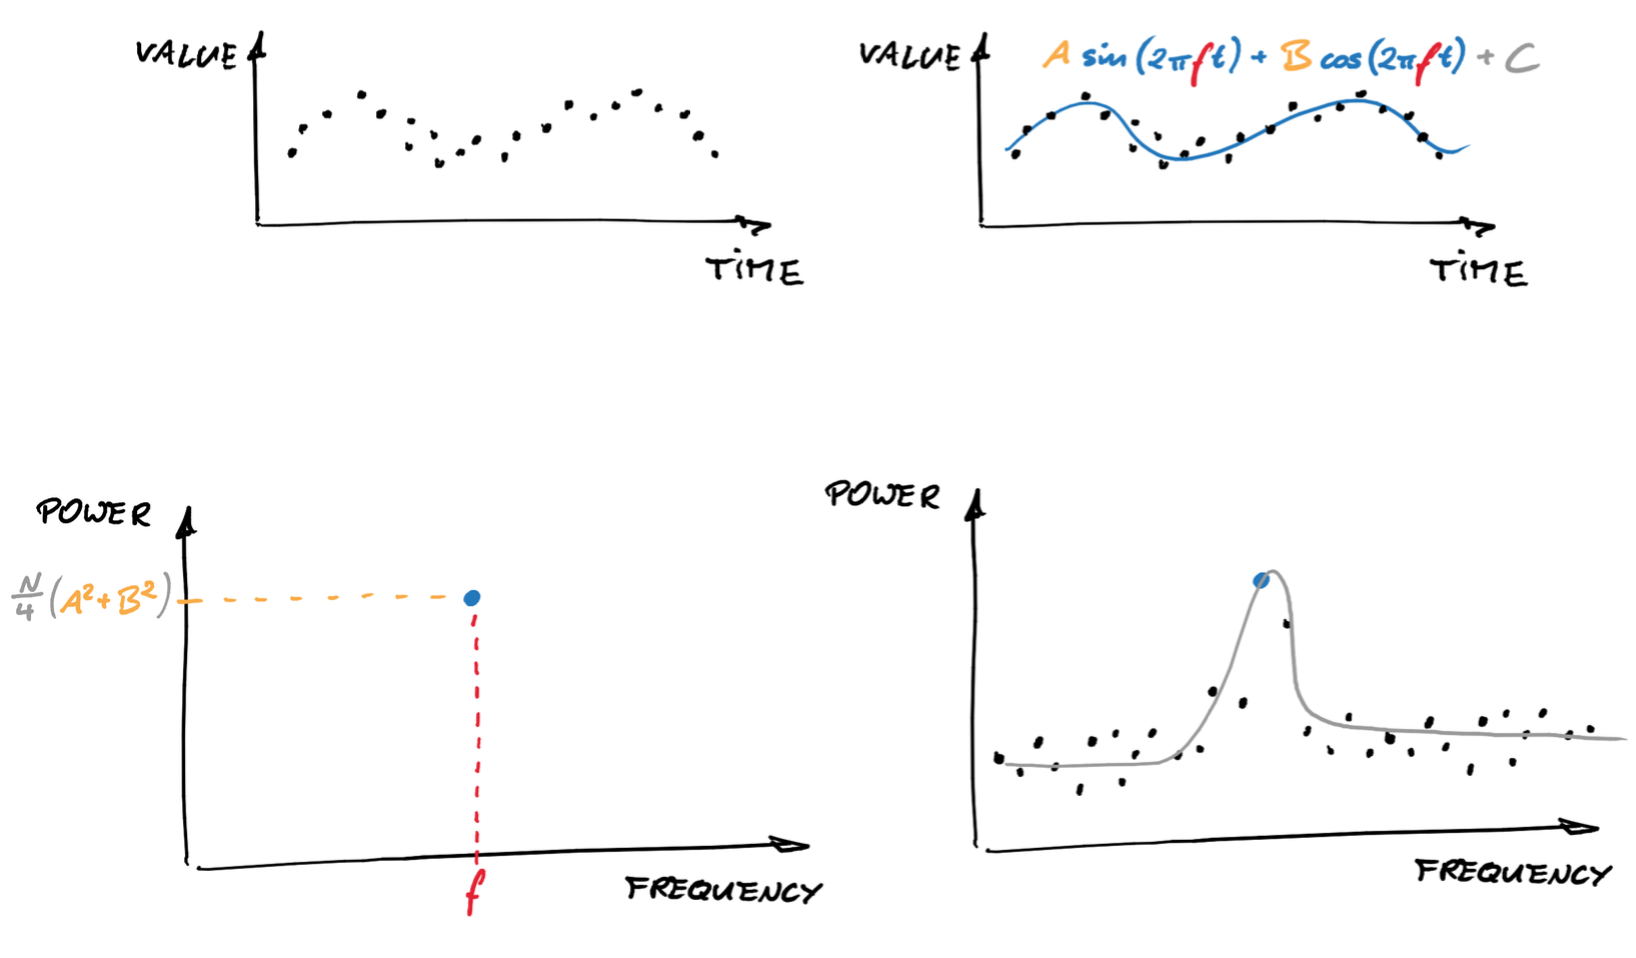
\includegraphics[width=\linewidth]{gfx/axions/LSSA}
  \caption{The LSSA periodogram, a function of frequency, is constructed by performing a linear least--squares fit at each of those frequencies.}
  \label{fig:LSSA}
\end{figure}


\subsection{Choice of frequencies}
The LSSA periodogram can be evaluated at any frequency. We are going to motivate the choice of a set of frequencies.

Every kind of spectral analysis is fundamentally limited by \emph{spectral resolution} (also referred to as \emph{bandwidth resolution}), which is approximately equal to the inverse time separation between the first and the last measurement. If the LSSA power is evaluated more densely than that, the results are expected to be highly correlated. Additionally, if the LSSA periodogram stretches beyond approximately half of the sampling frequency \note{MR: sampling frequency is not even well defined in our case}, following the reasoning similar to the Nyquist--Shannon sampling theorem \note{MR: citation needed?}, aliasing is expected to occur, introducing correlations between points of the periodogram.

We do not make special effort to avoid sampling frequencies where spurious power fluctuations will be correlated. An exact treatment of the correlations is virtually impossible in our complicated case, when the measurements are neither equally--spaced nor point--like. We prefer to take the possible correlations into account, which gives us freedom when it comes to choosing the frequencies.

We want to choose the frequencies, such that (a) we cover a broad spectrum and (b) we are sure to detect an axion--induced peak, if it is in the covered spectrum. The coherence of the oscillating axion field is of the order of $10^6$ periods, which translates into a relative width of the peak they would produce in the periodogram of $10^{-6}$. The spectral resolution of the ILL data set is the inverse of 1545 days ($\approx \unit[7.5 \cdot 10^{-9}]{Hz}$), which means that above frequencies of above $\unit[7.5 \cdot 10^{-3}]{Hz}$ the width of the peak is not resolvable. As we do not attempt to stretch beyond this frequency, the spacing between frequencies has to be at most equal to the spectral resolution.

As the highest frequency we choose approximately 10 times per day ($\unit[10^{-4}]{Hz}$) \note{MR: to be filled by NA}. We have one data point approximately every day. For frequencies higher than that, the sensitivity quickly drops and the computational needs rise. We cover the space between zero (exclusive) and the highest frequency with linearly spaced frequencies separated by one spectral resolution. This gives us $\sim 10^6$ frequencies to analyse. In order to stretch our results in the low--frequency direction, we add 100 logarithmically spaced frequencies below one spectral resolution. As the lowest frequency we choose the frequency that would correspond to an axionlike particle of mass $\unit[10^{-24}]{eV}$ ($\unit[9.54 \cdot 10^ {-9}]{Hz}$) \note{MR: to be filled precisely by NA}. \note{YS: Shouldn't the inverse of 20 years correspond to a much smaller frequency, or are we talking about something different here? NA: inverse of 20 years should be much less than $10^-4$Hz, I have changed to show the actual lowest frequency I use. I have justified it in terms of axion mass, but maybe if we are presenting a limit on oscillating EDMs with an interpretation in terms of alp couplings we should use a different justification or lower frequency} Thereby a set of $N$ angular frequencies $\omega_i$ is constructed.


\subsection{Null hypothesis test}
In the run--level analysis, the time series is the neutron electric dipole moment $d_n$ measured in each run of the ILL experiment. We calculate the LSSA periodogram of this series. A signature of an oscillating signal would be a peak in the periodogram. Precisely, we want to answer the question:

\begin{center}
  \emph{How likely is it that the highest peak in the periodogram is not only a random fluctuation?}
\end{center}

We are, in fact, interested in the \emph{least likely} peak, which may not be equivalent to the highest one. For clarity we are going to be first considering the highest peak, and explain the difference later.\note{NA: in final PRL we should probably dive straight in talking about the least likely peak.}

To describe the question mathematically, let us denote the time series of the real data by $D$. The peridogoram is then a set of $P^D(\omega_i)$. We are interested in \emph{the maximum of the periodogram}:
\begin{align}
  P_{max}^D &:= \mathrm{max}_i\,P^D(\omega_i) \\
  \omega_{max}^D &:= \mathrm{arg\,max}_{\omega_i}\,P^D(\omega_i)
\end{align}
The height of the maximum, $P_{max}^D$, is a statistic itself. We refer to it as \emph{global}, in contrast with the \emph{local} statistics $P^D(\omega_i)$. We consider the distribution of $P_{max}^{H_0}$ given the null hypothesis $H_0$, where the time array is an array of normally distributed random variables, with widths equal to the corresponding error--bars. The probability that a peak at least as high as the one observed arises as a random fluctuation is:
\begin{equation}
  % \mathrm{Pr}\left( P_{max}^{H_0} > P_{max}^D\ |\, H_0 \right) \ .
  \mathrm{Pr}\left( P_{max}^{H_0} > P_{max}^D \right) \ .
\end{equation}
This value is called the \emph{false alarm probability} (see eg. \cite{Pandola2004}). It can be numerically calculated with the Monte Carlo method by generating random data according to the null hypothesis (Fig.\,\ref{fig:generating_null_hypothesis_periodogram}) and counting the relative number of cases when $P_{max}^{H_0} > P_{max}^D$. To claim a discovery, the \emph{false alarm probability} has to be at most in the range of $2.87\,\cdot\,10^{-7}$ (so--called 5--sigma) \cite{PDG2014}.

\begin{figure}[htb]
  \centering 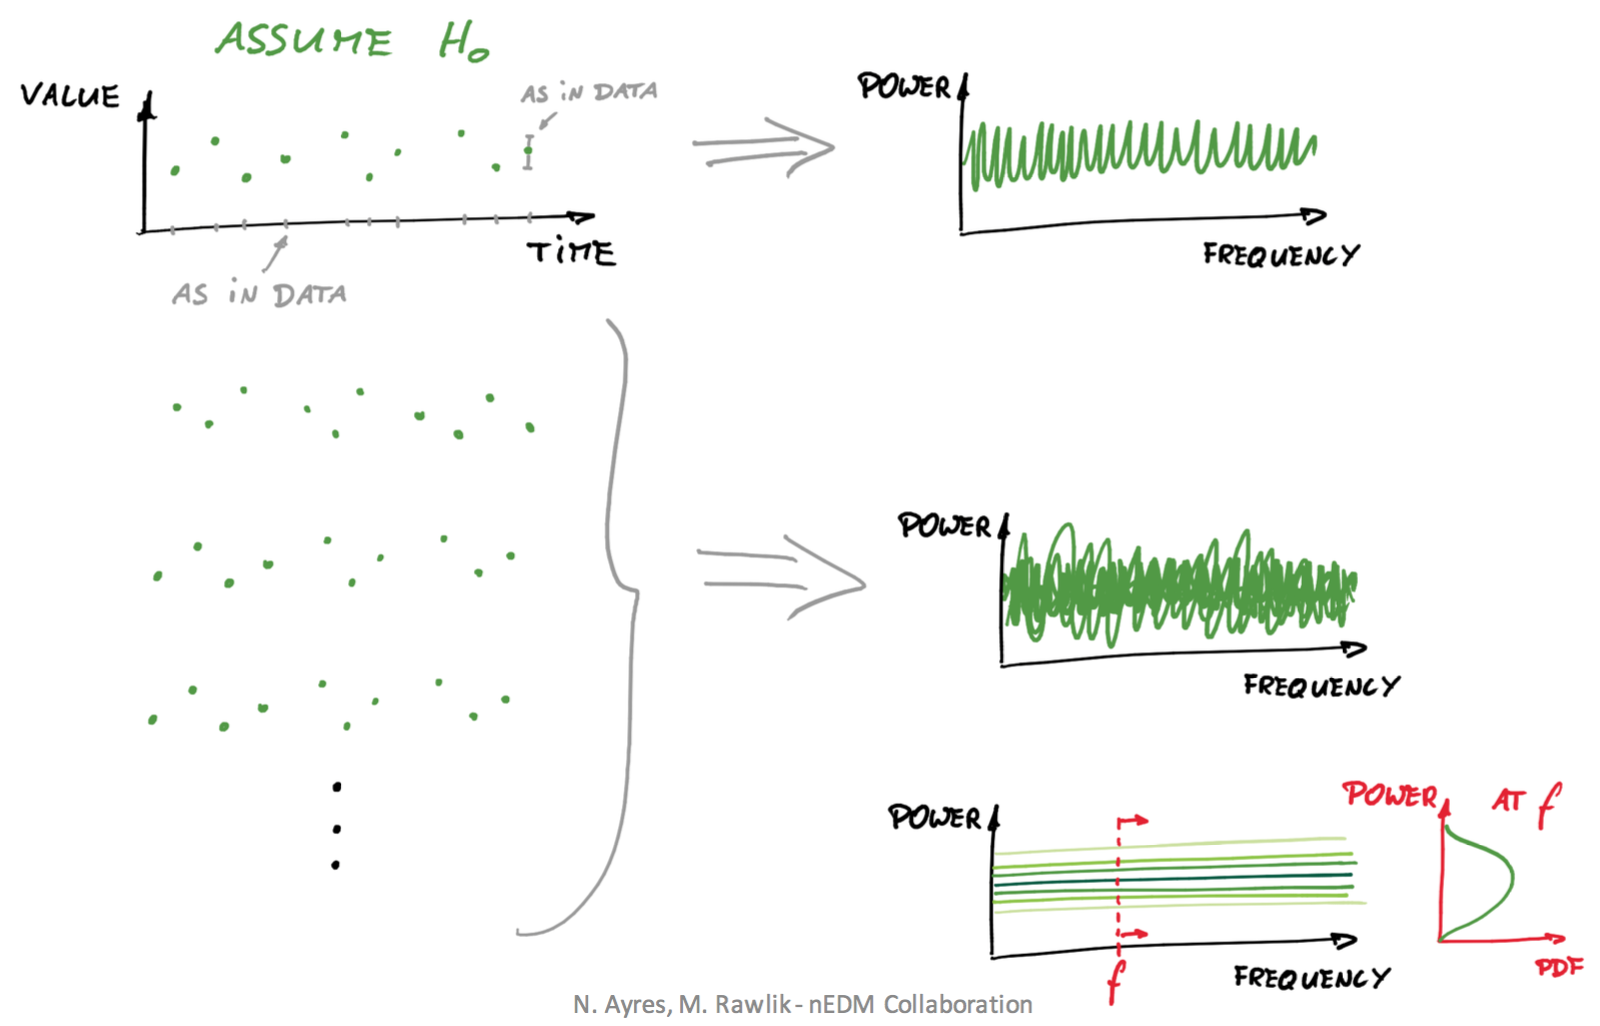
\includegraphics[width=\linewidth]{gfx/axions/null_hypothesis.png}
  \caption{The distrbution of LSSA periodogram for the null hypothesis is generated with a Monte--Carlo method. As the periodogram is a one--dimensional function, its distribution is two--dimensional.}
  \label{fig:generating_null_hypothesis_periodogram}
\end{figure}

It should be stressed that the distribution of $P_{max}$ is very different from the one of $P(\omega_{max})$. By looking for the highest peak, we check a big number of random variables $P(\omega_i)$ and pick a very special one --- the one that does lie the furthest in the tail of the distribution. The distribution of $P_{max}$ thus is centred around much higher values, as shown in Fig.\,\ref{fig:max_power_distribution}.

\begin{figure}[htb]
  \centering 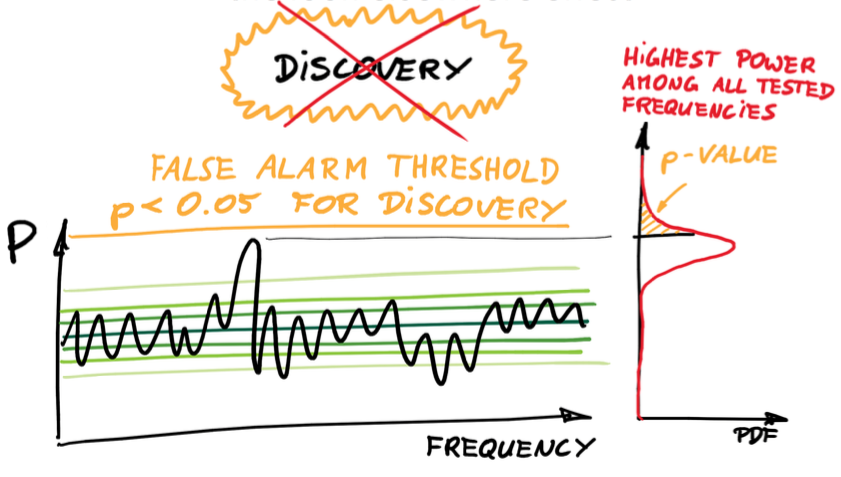
\includegraphics[width=\linewidth]{gfx/axions/max_power_distribution.png}
  \caption{The distribution of \emph{highest power} in a periodogram is centered much higher then the distributions of power in the periodogram.}
  \label{fig:max_power_distribution}
\end{figure}

\note{MR: might consider a better notation} As already mentioned, we are really interested in the \emph{least--likely} peak. Only if the noise--bed (the null hypothesis periodogram) is flat, then the highest peak corresponds to the least--likely peak. The cumulative distribution function (CDF) of power at frequency $\omega_i$ can be estimated by evaluating $P(\omega_i)$, $P_i$ for short, for many signals generated assuming $H_0$. We denote the CDF by $F_{P_i}$. The \emph{local} p-value for the compatibility of $P^D(\omega_i)$ with $H_0$ is simply:
\begin{equation}
  p_i = 1 - F_{P_i}(P^D_i)
\end{equation}
The \emph{local} p-value for the least--likely peak is:
\begin{equation}
  p_{\mathrm{min}} = \mathrm{min}_i \, p_i
\end{equation}

The question is what is the \emph{global} p-value of the least likely peak in the data--set being compatible with $H_0$. If the points of the periodogram were not correlated, this would be a simple case of many hypothesis testing \cite{Algeri2016}. The local p-values $p_i$ are, by definition, uniformly distributed. The CDF of a maximum of a set of uncorrelated variables is a product of their CDFs \note{MR: Cite Papoulis 1965, 7.1, application 3 - taken from Scargle III a)}. So in this case we have:
\begin{align}
  F_p(p) &= p \\
  F_{p_{max}}(p) &= p^N \\
  &\text{with}\ p' := 1 - p :\\
  F_{p_{min}}(p) &= 1 - F_{p'_{max}}(p') = 1 - (1 - p)^N \label{eq:Fpmin}\\
\end{align}
where $N$ is the number of frequencies. Correlations in the periodogram effectively lower $N$. If three dice are rolled in a way that two always give the same result, this is the same as rolling two dice when minimum roll is concerned. To quantify that, we exploit the fact that we can do fast Monte Carlo and \emph{simulate} the whole process: generating many signals assuming the null--hypothesis and calculating the p-value of the least--likely peak. Thereby we can estimate the CDF of $p_{\mathrm{min}} \, | H_0$, which we call $F^g$. Then the \emph{global} p-value is given by:
\begin{equation}
  p^g = F^g(p_{\mathrm{min}}^D)
\end{equation}

We can further determine \emph{false--alarm} thresholds. Traditionally, they are chosen to be at p-values of the normal distribution at $n \,\sigma$. The \emph{global} threshold p-value we call $p^g_{f.a.}$. The \emph{local} threshold p-value is:
\begin{equation}
  p_{f.a.} = \left( F^g \right)^{-1}(p^g_{f.a.})
\end{equation}
For each frequency the threshold power can be calculated:
\begin{equation}
  P^{f.a}_i = F_{P_i}^{-1}(1 - p_{f.a.})
\end{equation}
We claim a statistically significant discovery if the periodogram of the $d_n$ time--series crosses the 5--sigma false--alarm threshold.

The amount of Monte Carlo samples can be reduced, if the CDFs can be extrapolated. Effects like unequal error--bars and measurements of non--negligible duration causes them to deviate from the strictly derived equations in \cite{Scargle1982}. Nevertheless, we assume that functional form of the tails is preserved. Under the null hypothesis $F_{P_i}$ has form $1 - e^{-P}$ \cite{Scargle1982}. For $F^g$ we assume a form of Eq.\,(\ref{eq:Fpmin}), where $N$ is a parameter that we have to fit to account for correlations in the periodogram.

In Fig.\,\ref{fig:ILL_detection} we present the periodogram of a fake ILL dataset (geneated with the same run timings and uncertainties as in the real dataset, with run EDM values generated according to gaussian distribution with mean of $0$ and standard deviation equal to that run's uncertainty). We decided not to analyse the real data set until we are fully happy with the method.

\begin{figure}[h!]
  \begin{center}
    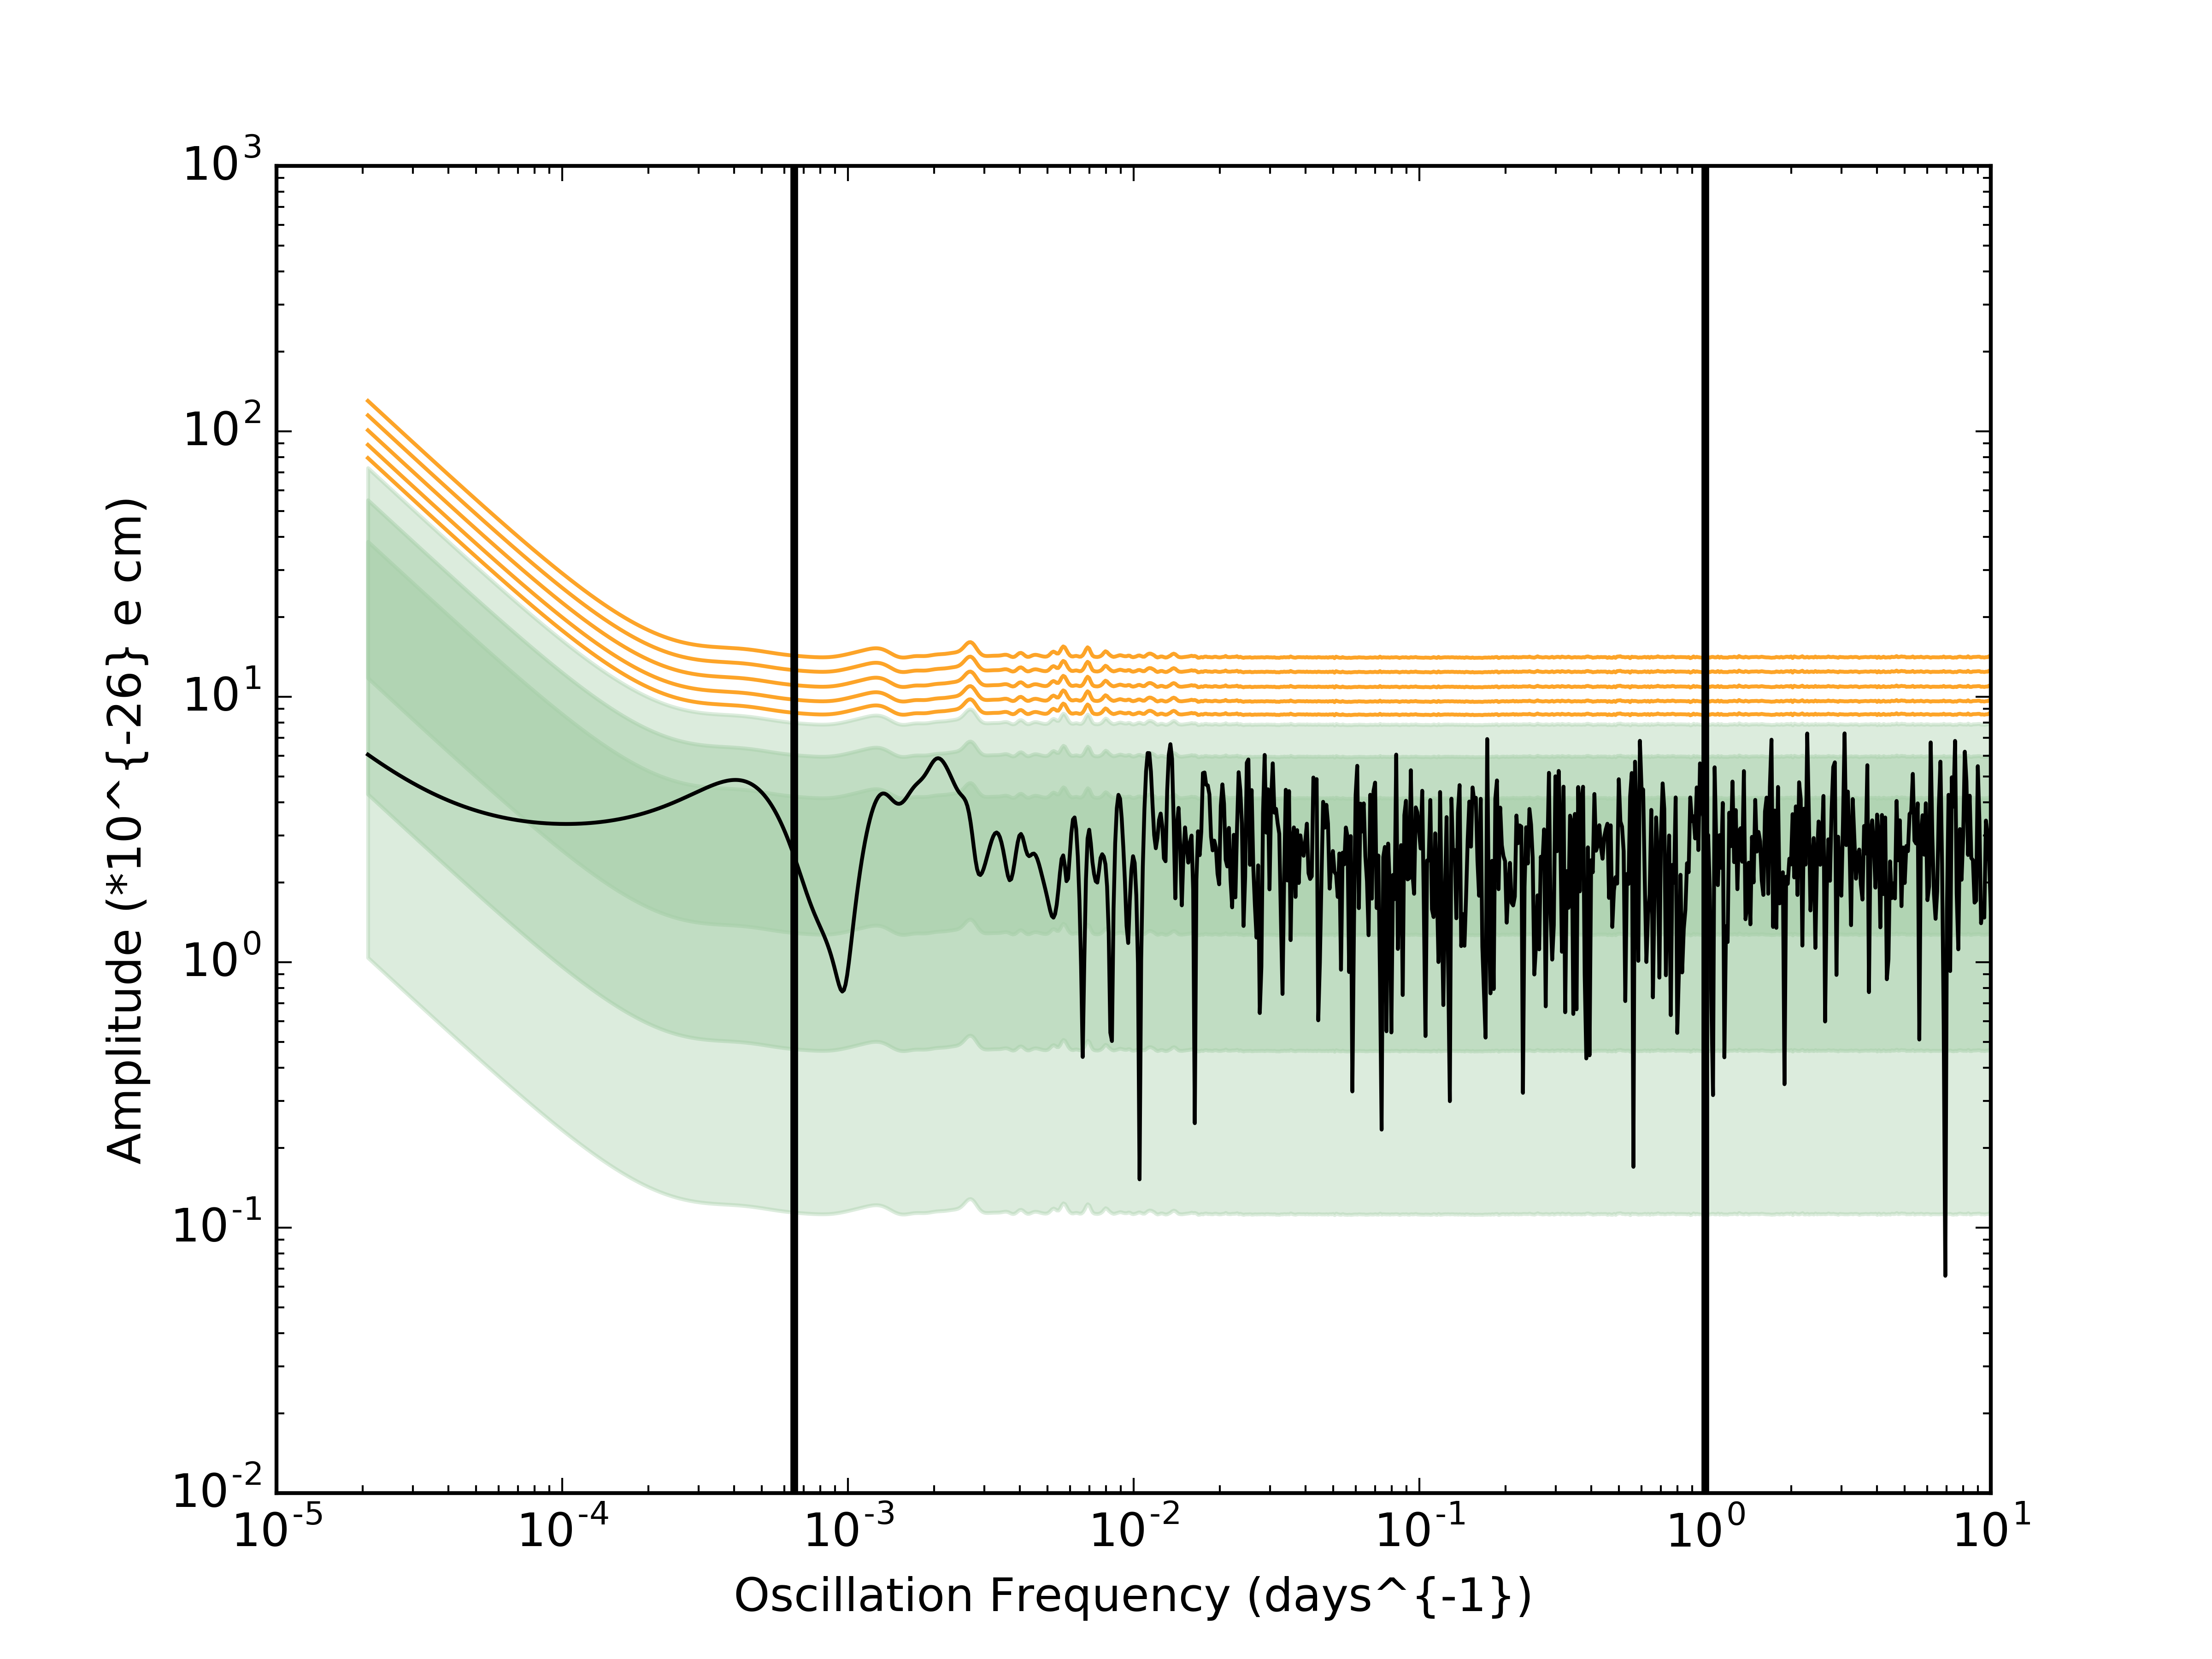
\includegraphics[width=\columnwidth]{gfx/axions/ILL_detection_Periodogram.png}
    \caption{Periodogram of a fake ILL dataset. The green bands represent the distribution of the periodogram given the null hypothesis. The orange lines are 1-, 2-, 3-, 4-, 5--sigma false--alarm thresholds.}
    \label{fig:ILL_detection}
  \end{center}
\end{figure}

\note{MR: here should go the discussion of the result.}


\subsection{Exclusion region}
\begin{figure}[htb]
  \centering 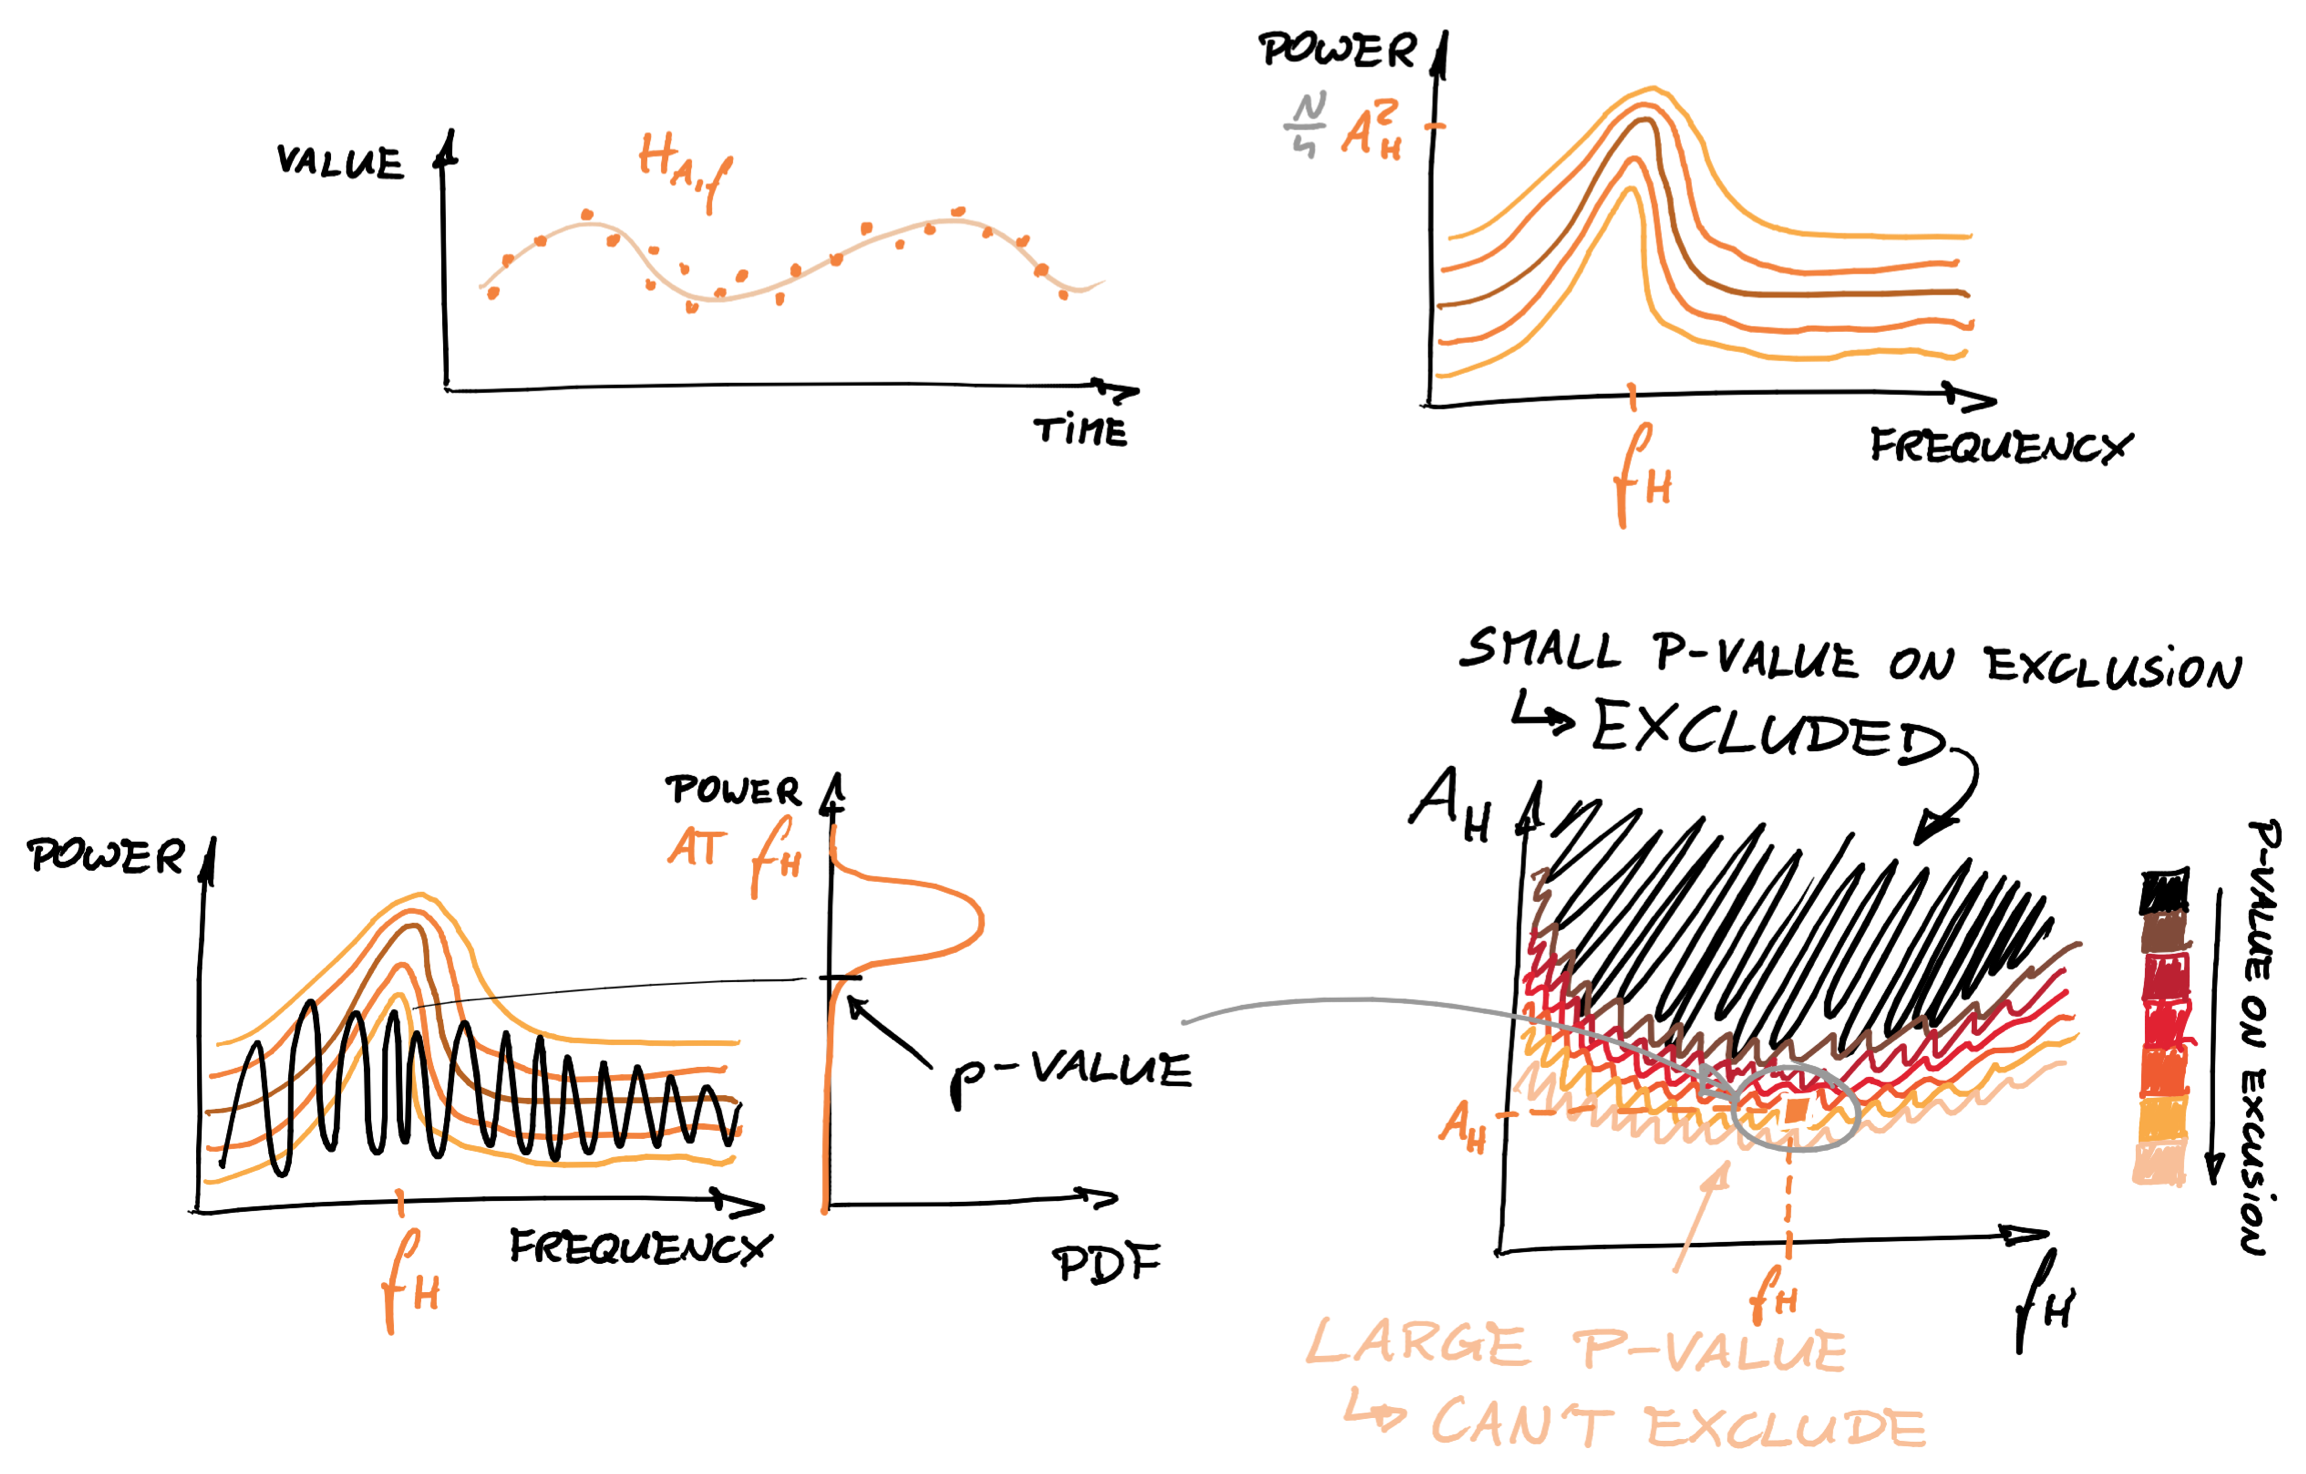
\includegraphics[width=\linewidth]{gfx/axions/exclusion_region.png}
  \caption{Determining the exclusion limit. Note that in practice not the whole periodogram needs to be generated, but only its slice at $f_H$.}
  \label{fig:exclusion_region}
\end{figure}

Should no claim for a discovery be possible, the next question to ask is:
\begin{center}
  \emph{Which oscillations would produce a significant peak, but did not, and can be thus excluded?}
\end{center}
In order to answer this question, the data need to be tested against being compatible with a number of model signal hypotheses. As an oscillation is characterised by its amplitude and frequency, the space of the alternative hypotheses to test is two--dimensional.

The probability that a hypothetical oscillation of amplitude $A$ and frequency $\omega$ would produce less power at frequency $\omega$ then observed is:
\begin{equation}
  % \mathrm{Pr}\left( P(\omega) < P^D(\omega)\ |\, H(\omega, A) \right) \ .
  \mathrm{Pr}\left( P^{H(\omega, A)}(\omega) < P^D(\omega)\ \right) \ .
\end{equation}
This probability is the p-value for the hypothesis $H(\omega, A)$ rejection. The distribution of $P^{H(\omega, A)}(\omega)$ is obtained with the Monte Carlo method. Here we also make use of CDF tail extrapolation \note{MR: This time, however, we extrapolate the low-power tail}, assuming a functional form as eq.\,(15) in \cite{Scargle1982} \note{MR: Not strictly, though. This equation behaves like linear function for very small $z$}. This test is repeated for different $\omega$ and $A$, each time covering a \emph{pixel} of the space of possible hypotheses. This procedure is shown schematically in Fig.\,\ref{fig:exclusion_region}. The set of hypotheses excluded at most at certain p-value forms an \emph{exclusion region}. We take the threshold p-value to be 5\%, which corresponds to a traditional confidence level of 95\%.

In this case, we cover the frequency spectrum much less densely than is the case in the null hypothesis test. This procedure is essentially evaluating the sensitivity of the measurement, which is solely determined by the timing and precision of the measurement points. We do not expect any highly resonant structures to appear therein.

During the Monte Carlo simulations we assume a perfectly coherent signal. The width of a real peak is not resolvable, as already mentioned.

\begin{figure}[htb]
  \begin{center}
    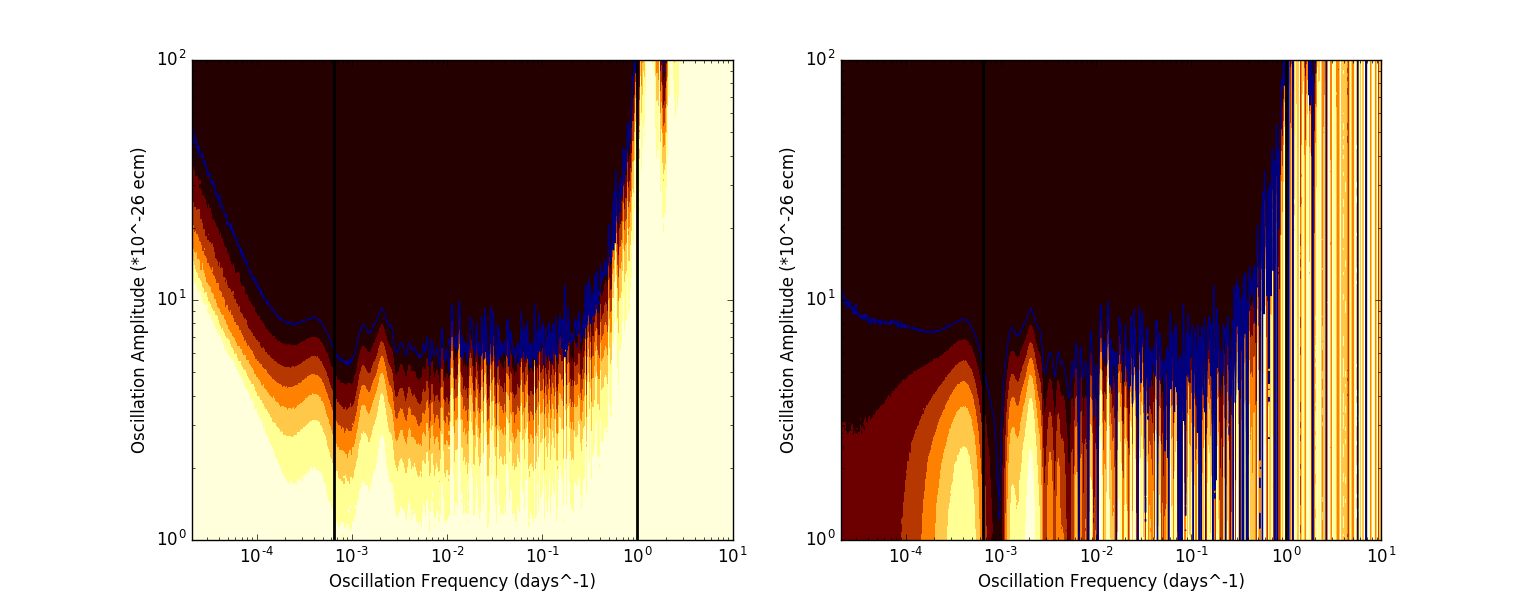
\includegraphics[width=\columnwidth]{gfx/axions/ILL_p_signal_and_cls_sensible.png}
    \caption{p-value on the alternative hypothesis rejections evaluated for the fake ILL dataset. The CLs method has been used. \note{MR: To be illustrative, I would present two versions of this figue, side--by--side: without the CLs method and with (as in Fig.\,\ref{fig:exclusion_no_CLs}, which would be then omitted).}}
  \label{fig:ILL_exclusion}
  \end{center}
\end{figure}

\begin{figure*}[htb]
  \centering 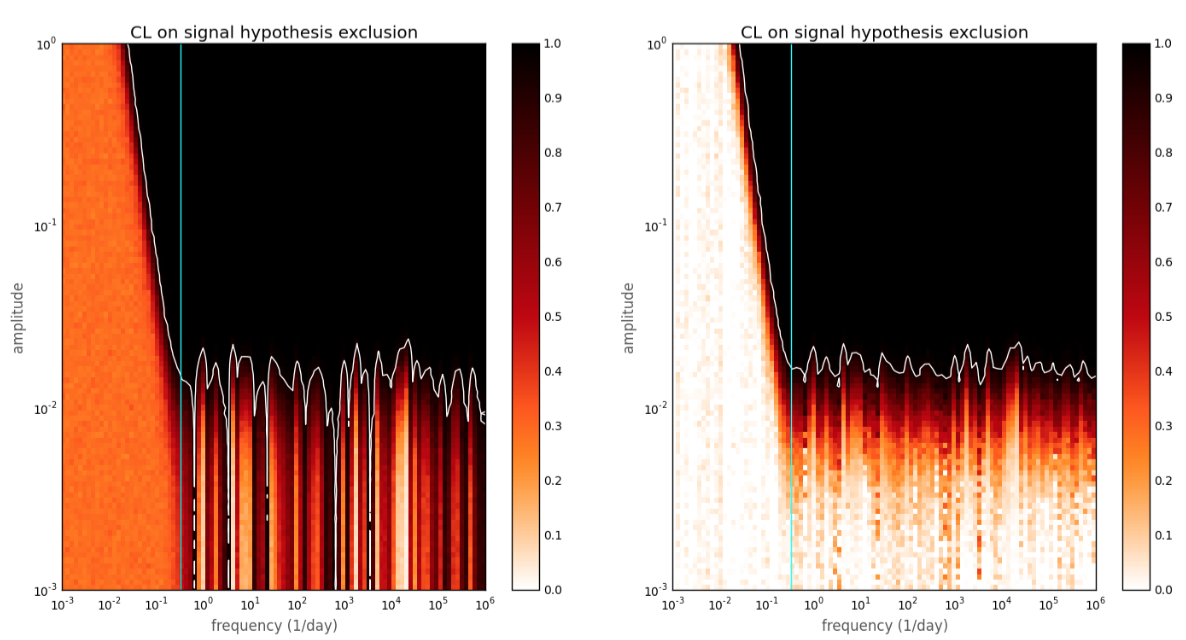
\includegraphics[width=\linewidth]{gfx/axions/exclusion_no_CLs.png}
  \caption{Confidence level \note{MR: need to establish whether we use CL or p-value} on rejection of various signal hypotheses, spanned by their amplitude and frequency. \emph{Left:} without the CLs method, \emph{right:} with the CLs method. The plots were produced with a test dataset, very different from the ILL dataset. The picture for the appropriate fake ILL dataset is in Fig.\,\ref{fig:ILL_exclusion}}.
  \label{fig:exclusion_no_CLs}
\end{figure*}

The result of this procedure applied to a fake ILL dataset is presented on the left--hand side in Fig.\,\ref{fig:ILL_exclusion}. Looking at the exclusion region, one sees that the sensitivity to exclude drops for both high and low frequencies. This can be understood by looking at Fig.\,\ref{fig:sensitivity}, where the power obtained in the Monte Carlo generation for various hypotheses is plotted on top of the signal periodogram. For hypotheses with the same assumed amplitude of oscillation, the amplitude seen in the periodogram is constant for periods between the separation of the data points and the total length of the data set. Longer periods are harder to exclude, as it is always possible that one is near an antinode of an extremely slow oscillation. This manifests itself as a high amplitude seen even when the null hypothesis is assumed. High frequencies are suppressed because the experiment measures the average of the oscillation over a run. There little amplitude is visible, despite assuming an oscillation of a large amplitude. In particular there are dips at the approximate sampling frequency (the data have not been taken perfectly regularly) and its multiples.

\begin{figure}[htb]
  \centering 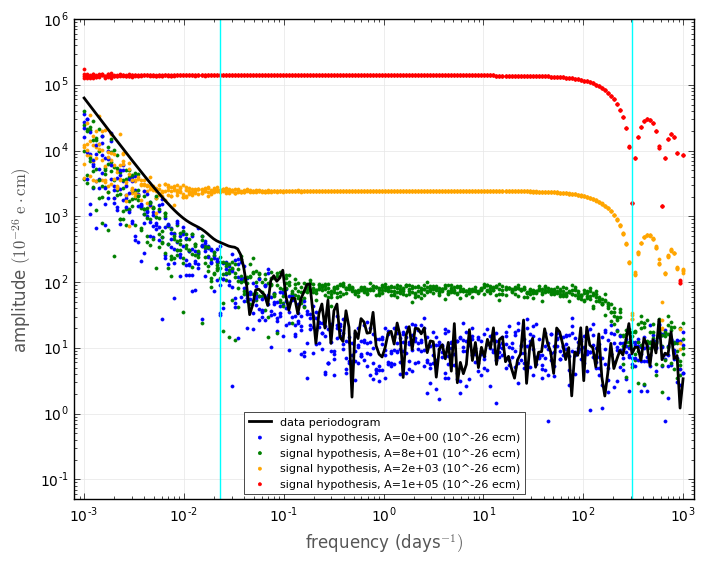
\includegraphics[width=\linewidth]{gfx/axions/sensitivity.png}
  \caption{For each frequency $f$, $\sqrt{\text{power}}$ is plotted for the dataset (black line) and MC--generated signal hypothesis of frequency $f$ and various amplitudes (different colours). For both high and low frequencies, the MC results approach the null hypothesis (blue). Also, a dip in power is nicely visible for oscillations coherent with the sampling frequency (and its multiples). The vertical lines depict the time--span of the dataset and the median separation between centres of runs.  The plot was produced with a test dataset, very different from the ILL dataset. \note{MR: It would be good for the sake of consistency to produce such a figure for the ILL fake dataset. - see fig \ref{fig:ILL_sensitivity}}}
  \label{fig:sensitivity}
\end{figure}

\begin{figure}[htb]
  \centering 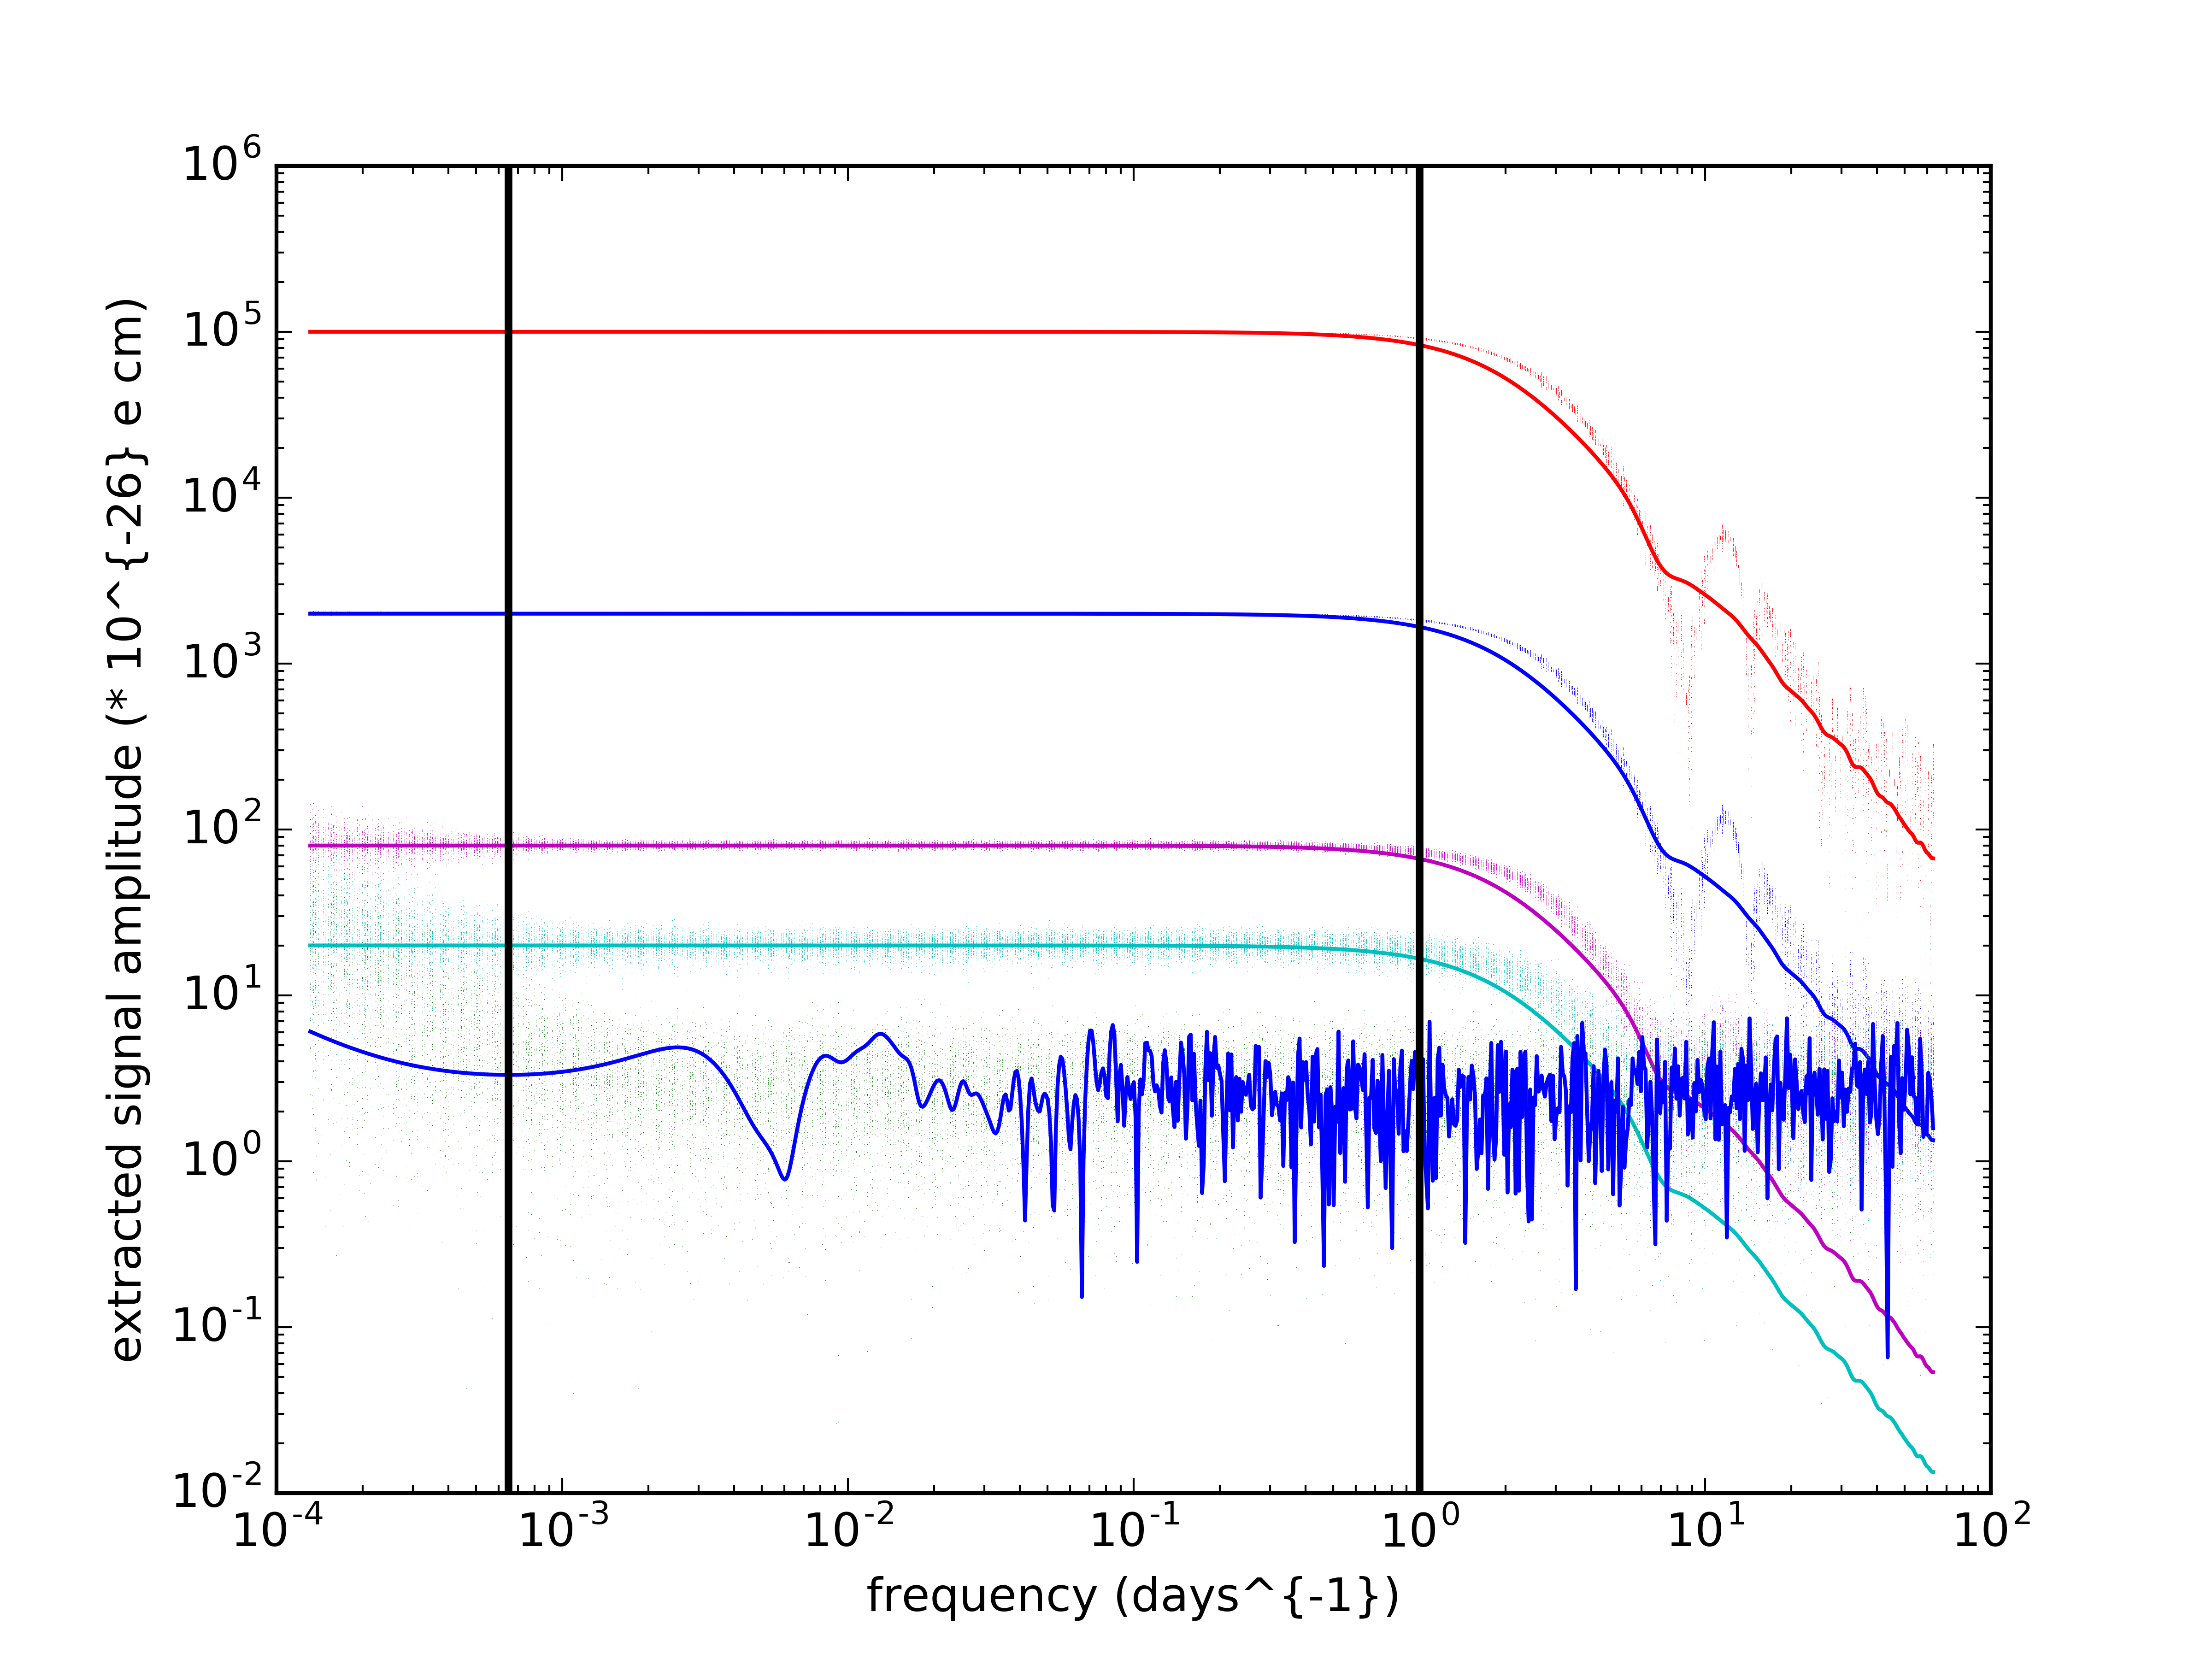
\includegraphics[width=\linewidth]{gfx/axions/ILL_signal_response_plot.png}
  \caption{The same plot as figure \ref{fig:sensitivity} for the ILL dataset}
  \label{fig:ILL_sensitivity}
\end{figure}


The 95\%~C.L. exclusion region, depicted by a white line on the left--hand side in Fig.\,\ref{fig:exclusion_no_CLs}, exhibits a number of thin peaks going down in very low amplitudes. Seemingly, for some frequencies, signals with amplitude far below the sensitivity of the experiment are excluded. This is disturbing. Consider, however, that as the power was evaluated for many frequencies, inevitably at some of them, roughly 5\%, the power is low enough to be rejected at 95\%~C.L. even when tested against the null hypothesis. However completely fine from the statistical point of view, physicists do not accept a situation, where a hypothesis is rejected based on an experiment which was not sensitive to it. One possible solution is called the \emph{CLs method}. The method is defined, as well as the problem itself discussed, in the booklet of the Particle Data Group~\citep{PDG2014}. Here we only shortly present its idea graphically in Fig.\,\ref{fig:CLs}. With use of the \emph{CLs method} exclusion is suppressed in the region of low sensitivity, as shown on the right--hand side in Fig.\,\ref{fig:exclusion_no_CLs}.

\begin{figure}[htb]
  \centering 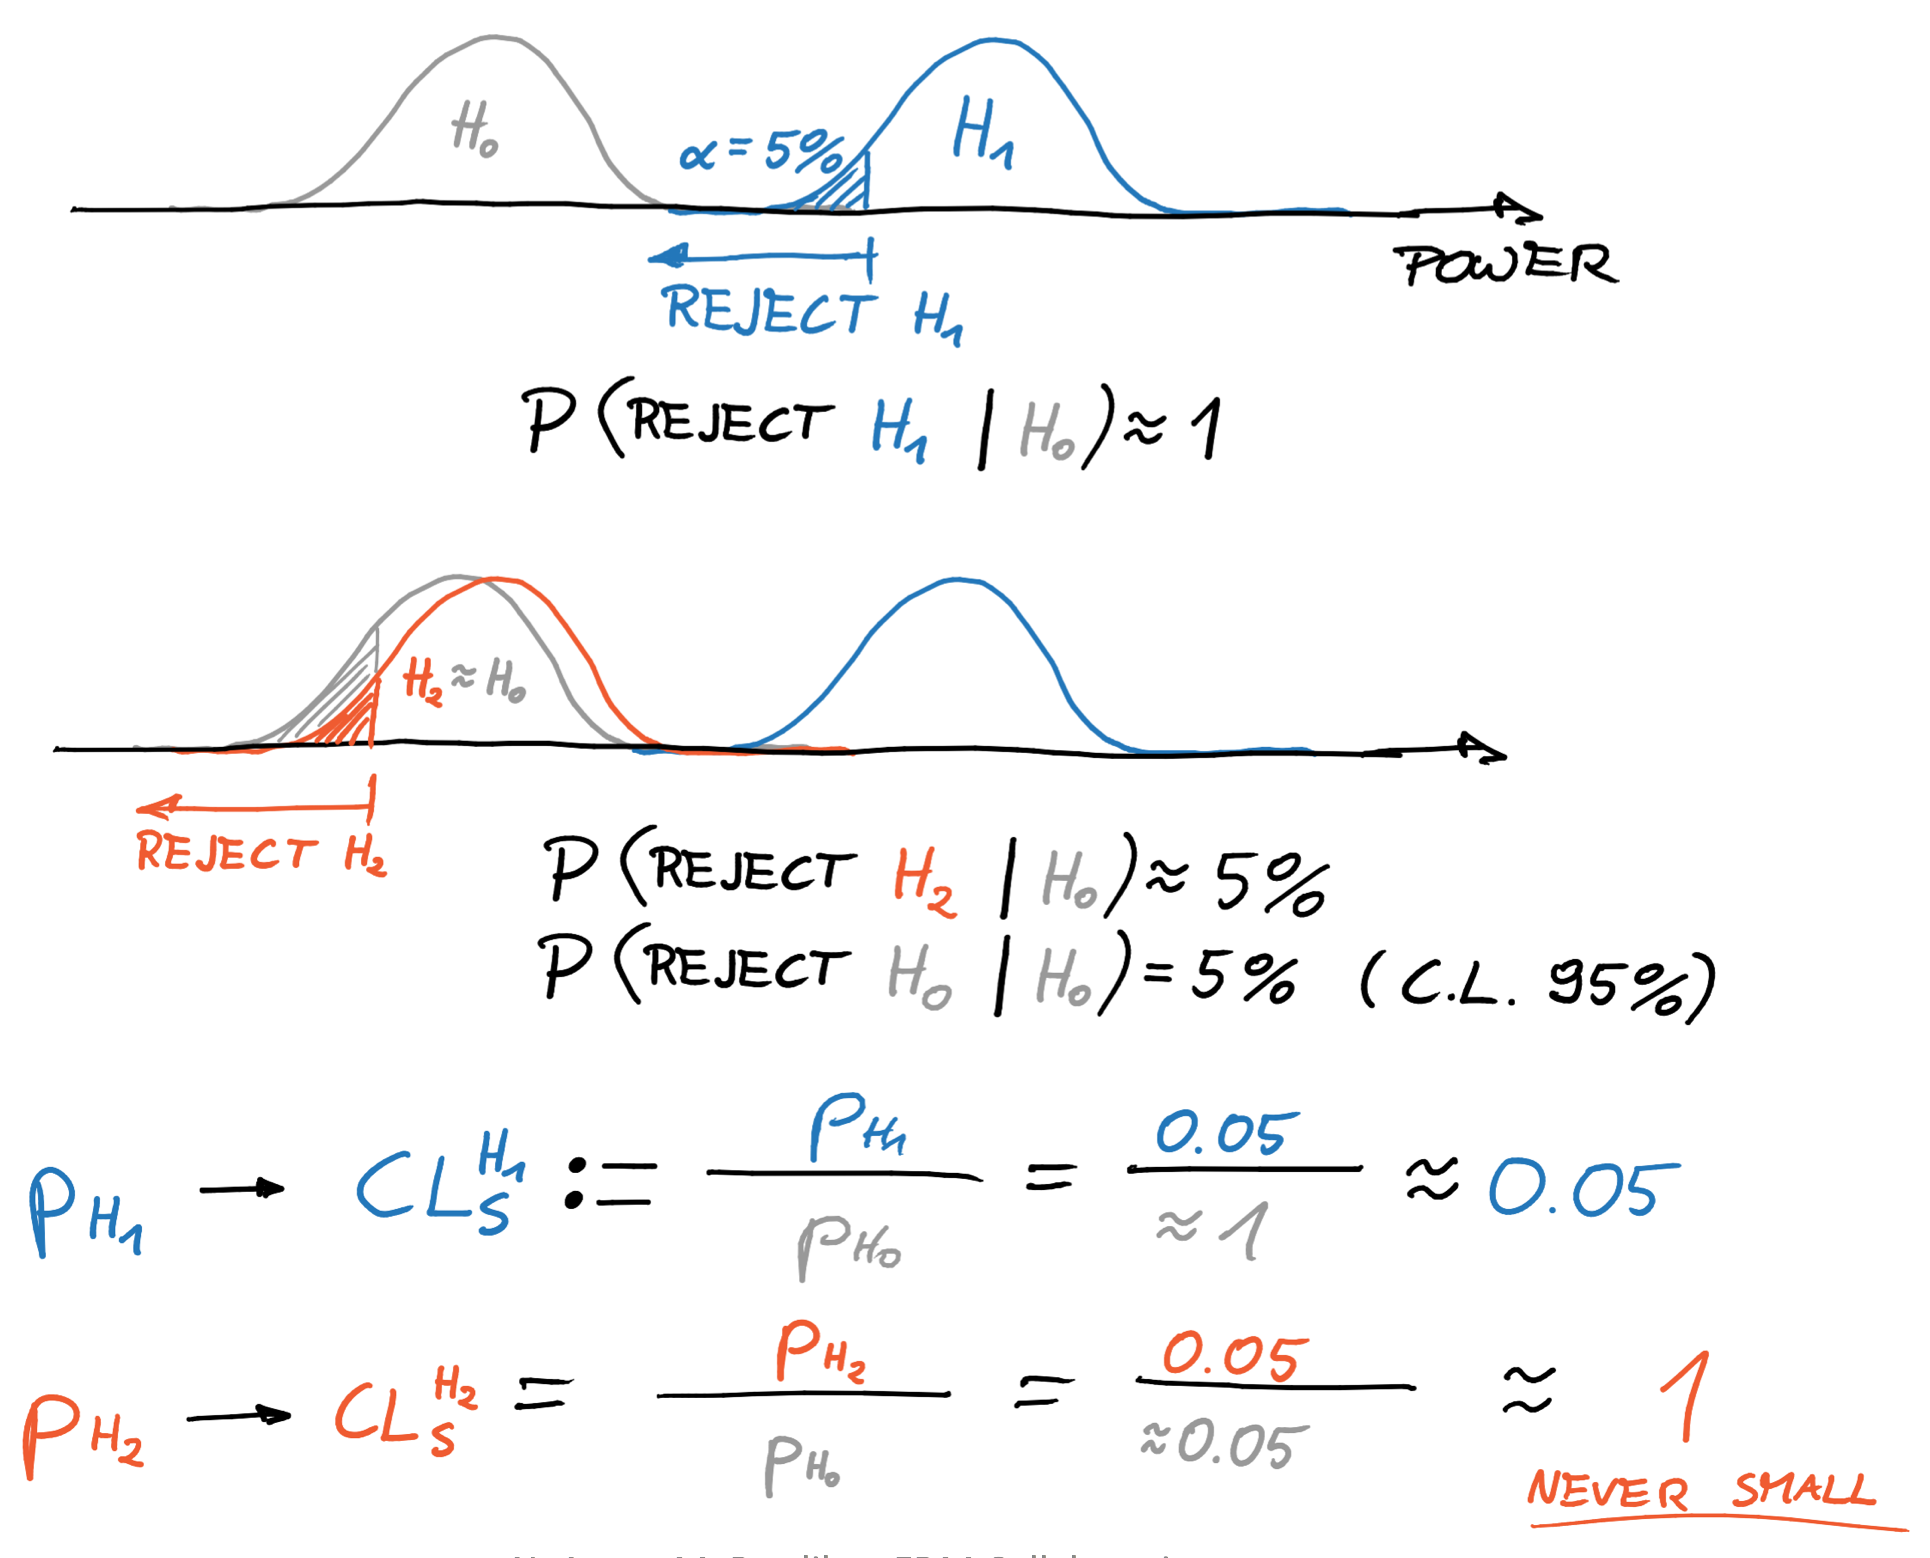
\includegraphics[width=\linewidth]{gfx/axions/CLs.png}
  \caption{The CLs method effectively suppresses power of hypotheses rejection if they are close to the null hypothesis.}
  \label{fig:CLs}
\end{figure}

Calculating each pixel of the alternative hypotheses space is largely a waste of resources. We are interested only in resolving the 95\% C.L. threshold. As a means of optimisation, we find the 95\% C.L. point for each frequency using the bisection algorithm. In only 10 steps it gives us relative precision below $0.01$ on its position. Thereby the final exclusion region is obtained \note{MR: figure needed, with the line only. It is missing for now for the run--level, but is present for the cycle--level}.


\subsection{Run--level Systematic Effects Discussion}
\note{To be filled by NA}. An analysis without a constant offset in the LSSA fit is possible if all known systematic effects that would cause a shift in the $d_n$ level are taken into account. In case of the ILL experiment, these have already been thoroughly studied for the mainstream nEDM analysis. A detailed reanalysis of all known systematic effects gave an overall systematic uncertainty of $\unit[0.38 \pm 0.99 \cdot 10^{-26}]{e\cdot cm}$ \cite{Pendlebury2015}. The central value was subtracted from the entire dataset, and the uncertainty on this value was considered small enough to be safely ignored, being around a tenth of the size of the oscillations we are sensitive to. This improves the sensitivity of the analysis to slow oscillations. \note{MR: We need to be absolutely sure that the exotic physics would NOT cause a shift, but only an oscillation around zero.} \note{YS: We are assuming that the only effects of exotic physics are due to the oscillating EDM here (with no extra static EDM), see footnote [39].}

The largest systematic effect in the ILL experiment

\note{MR: When we do that for the run--level analysis, we need to state the reason why is it not done for the cycle--level analysis. Possible reasons:
\begin{enumerate}
  \item Systematic studies are not yet finished.
  \item Maybe there is a reason why it is not at all possible. In run--level some systematic effects cancel when we bring the two field configurations (parallel and anti--parallel) together. In cycle--level they are considered separately.
\end{enumerate}
}

\note{MR: Another, more compact version of the run--level analysis description. \textbf{OUTDATED BY NOW}

  \subsection{Run--Level (ILL data) Least Squares Spectral Analysis}
  We are looking for oscillations by applying least--squares spectral analysis (LSSA) \note{MR: citation needed} to a time series of $d_n$ extracted from each run. Thereby a linear fit to the time series is performed with model:
  \begin{equation}
  	A\,\mathrm{cos}(\omega t) + B\,\mathrm{sin}(\omega t) + C
  \end{equation}
  Power at frequency $\omega$ is defined as $P(\omega) := A^2 + B^2$. We analyse a fixed set of 200 frequencies $\omega_i$ (although this number may increase in the future).

  In order to test the resultant periodogram against the null hypothesis, PDF of the latter is generated with Monte Carlo for each frequency $\omega_i$, assuming that points of the $d_n$ time series come from a normal distribution with width equal to the error--bars. Taking into account the look---elsewhere effect, false--alarm threshold at $\omega_i$ is set at $n$th \note{MR: need a number here} percentile of the obtained PDF \note{MR: cite solar neutrinos here}. The results are shown in Fig.\,\ref{fig:ILL_detection}.

  % \begin{figure}[h!]
  % \begin{center}
  % \includegraphics[width=\columnwidth]{ILL}
  % \caption{TODO}
  % \label{fig:ILL_detection}
  % \end{center}
  % \end{figure}

  In order to obtain the exclusion region we test many alternative hypotheses $H_s$. In each we assume a perfectly coherent signal of frequency $\omega_s$ (the axion field has coherence time of $\approx 10^6$ periods \note{MR: I think it belongs here, as here it really matters}), amplitude $A_s$ and random phase. We generate many time--series, taking for each point the model averaged over the duration of the run \note{MR: To be \textbf{really} proper we would average over the free precessions of the run. We don't do it because we're lazy (and it doesn't matter) or is the timing information not available? PH: The accuracy of the timing information was limited, since the DAQ computer relied on its internal clock - there was no comparison with external atomic clocks, and there could easily be drifts of seconds to minutes.  For shorter timescales, therefore, the PSI data are far superior.}. From the time--series we evaluate PDF of $P(\omega_s)$. We do a one--side test looking for unlikely small amount of power in the data periodogram.

  Additionally we employ the CLs method \note{MR: citation needed} to dampen exclusions in the insensitive region. Thereby the p--value of the alternative hypothesis test $p_s$ is normalised to the p--value of corresponding test of the null hypothesis $p_0$. We consider the hypothesis as excluded when $p_s / p_0 < 0.05$. Results are in Fig.\,\ref{fig:ILL_exclusion}.

  % \begin{figure}[htb]
  % \begin{center}
  % \includegraphics[width=\columnwidth]{ILL_exclusion}
  % \caption{TODO \note{MR: I would present this figure like this: light, pastel colours for the run--level with a thick line at p-value = 0.05. The cycle--level analysis I would put on the same figure, but only the thick line.}}
  % \label{fig:ILL_exclusion}
  % \end{center}
  % \end{figure}
}


\section{Short time--base analysis}
\subsection{The PSI nEDM experiment}
The Sussex--RAL--ILL apparatus was moved to PSI where, benefiting from a stronger UCN source, and upon numerous improvements continues to measure the nEDM with ever increasing precision.

The most important thing for this analysis upgrade is the deployment of a Cesium magnetometer array \note{MR: citation needed} around the precession chamber. They allow for continuous measurement of the vertical magnetic field gradient $\partial_z B_z$ and thus correcting for drifts of the vertical magnetic field gradient on a cycle--basis, as in \ref{eq:R}.

Also, the PSI experiment is timed with GPS--referenced clocks. Precise timing allows for performing the analysis at higher frequencies reliably. \note{MR: Do we need that really? Maybe not mention it.}

\subsection{Differences to the long time--base analysis}
Going to a cycle--level analysis presents new challenges. The $d_n$ value cannot be extracted on cycle--basis. The spectral analysis is performed on $R := \frac{f_n}{f_{\mathrm{Hg}}}$ instead, which already includes $^{199}\mathrm{Hg}$ comagnetometer's correction for magnetic field drifts. The axion signal would appear there as an oscillation of amplitude dependent on the electric and magnetic field configuration: $0$ for $E=0$, $\pm \ \frac{h\, \gamma_{Hg} \langle B_0 \rangle }{2 E}$ for the parallel and anti--parallel configuration of $\vec{E}$ and $\vec{B}$, respectively (see Figure\,\ref{fig:cycle-level_phase_flip}). \note{note: relative fluctuations of $B_0$ are on the level of $10^{-6}$}. These three datasets are analysed separately --- the two $E \neq 0$ datasets are sensitive to an axion particle, while $E=0$ is a control data set.

\begin{figure}[htb]
  \centering 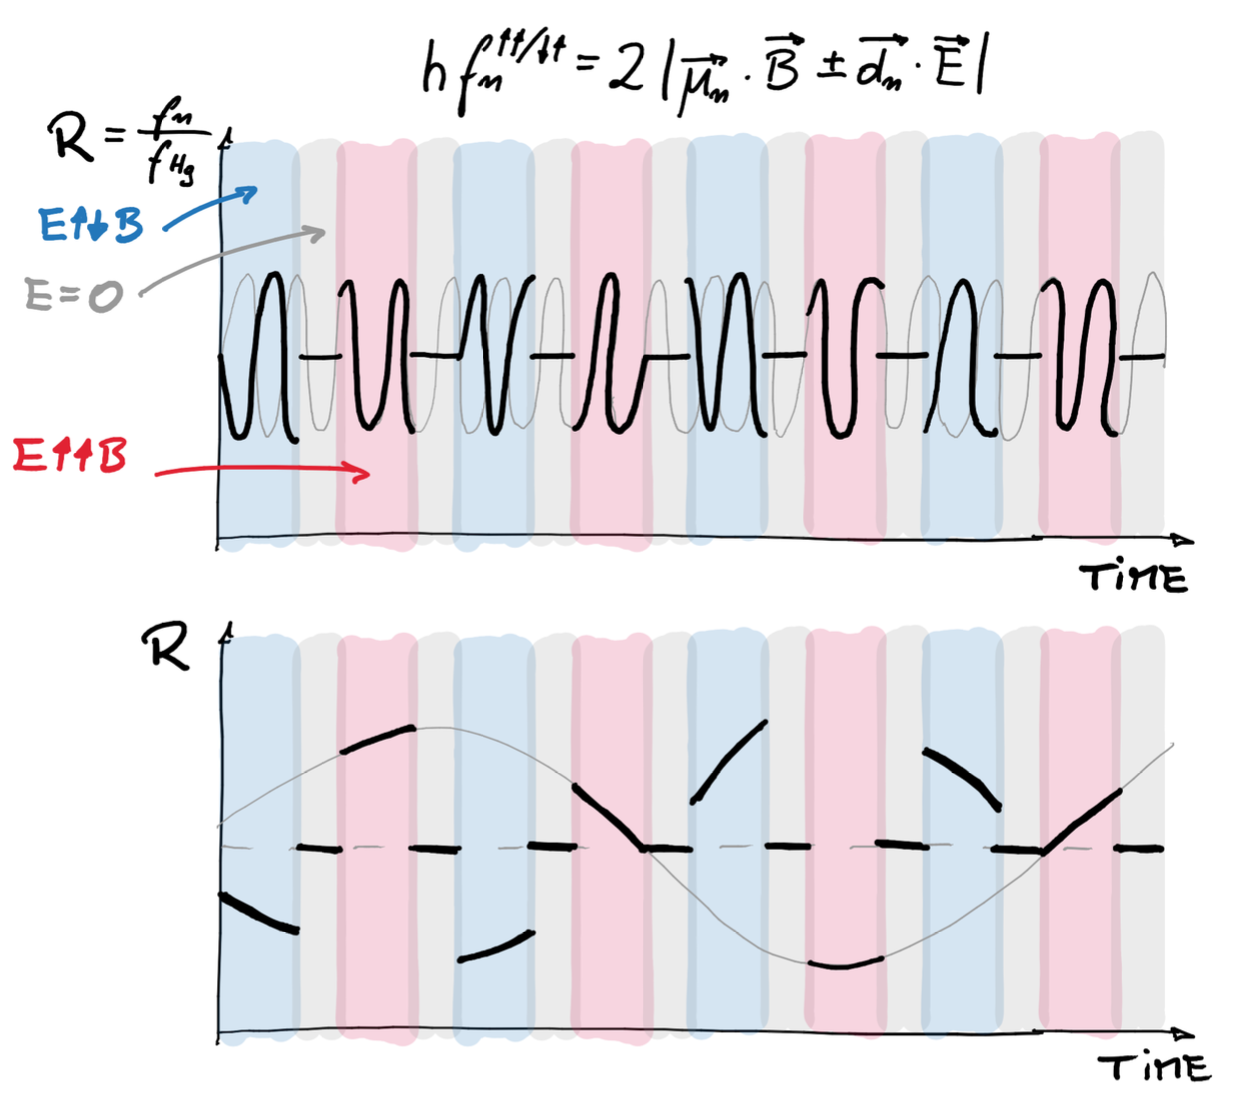
\includegraphics[width=\linewidth]{gfx/axions/cycle-level_phase_flip.png}
  \caption{A sketch of how an axion--induced signal would appear in the $R$ time--series.}
  \label{fig:cycle-level_phase_flip}
\end{figure}

The presence of a magnetic field gradient $\frac{\partial B_z}{\partial z}$ causes a shift in $R$ (see Eq.\,(\ref{eq:R})). While the constant component of the shift is rejected by the spectral analysis, the Cesium magnetometer array \note{MR: citation needed} is used to correct for drifts of the gradient. The standard measurement procedure of the PSI nEDM experiment involves deliberate setting of a vertical gradient and changing it from run to run, as shown in Fig.\,\ref{fig:cycle-level_gradient_jump}. Additionally, the Caesium magnetometers are calibrated after each change, which alters systematic offsets in their readout. For these reasons correction for the magnetic field gradient across different runs is potentially unreliable and has not been done. Instead, the offset parameter $C$ in the LSSA fit is allowed to be different in each run. Sensitivity in periods larger then one run is thus sacrificed, but in this region the run--level analysis delivers a better limit. Last, but not least, the majority of the PSI data is blinded \note{MR: citation needed} --- an unknown constant $d_n$ has been injected into the data. As the data are not going to be unblinded for this analysis only, we cannot assume zero constant $d_n$. This makes combining the datasets hard, as the axion--induced oscillation would not be centered around the $R$ value measured without the electric field, as sketched in Fig.\,\ref{fig:cycle-level_blinding_offset}. Performing the analysis separately on the three datasets with different field configurations: $E=0$, $E \uparrow \uparrow B$ and $E \uparrow \downarrow B$, combined with allowing for different offsets $C$ in each run, greatly simplifies the analysis.

\begin{figure}[htb]
  \centering 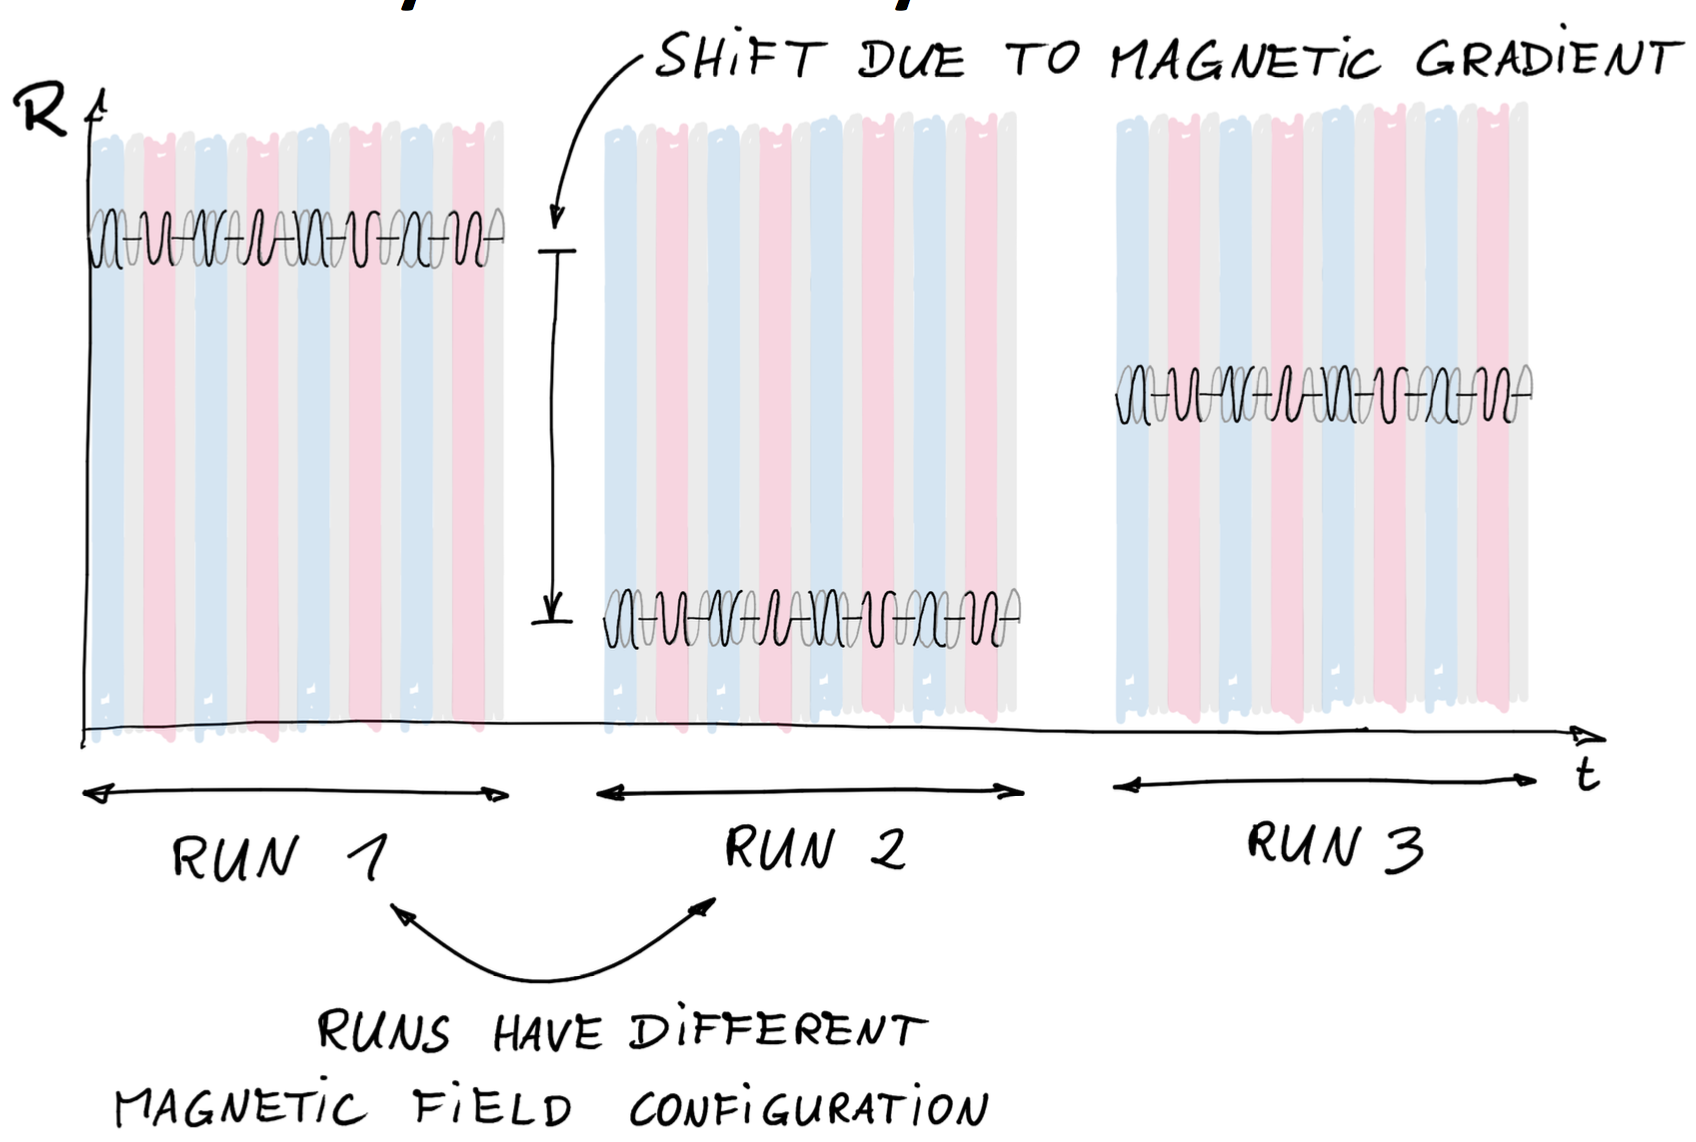
\includegraphics[width=\linewidth]{gfx/axions/cycle-level_gradient_jump.png}
  \caption{A sketch of how the $R$ time--series with an axion signal would look like across different runs.}
  \label{fig:cycle-level_gradient_jump}
\end{figure}

\begin{figure}[htb]
  \centering 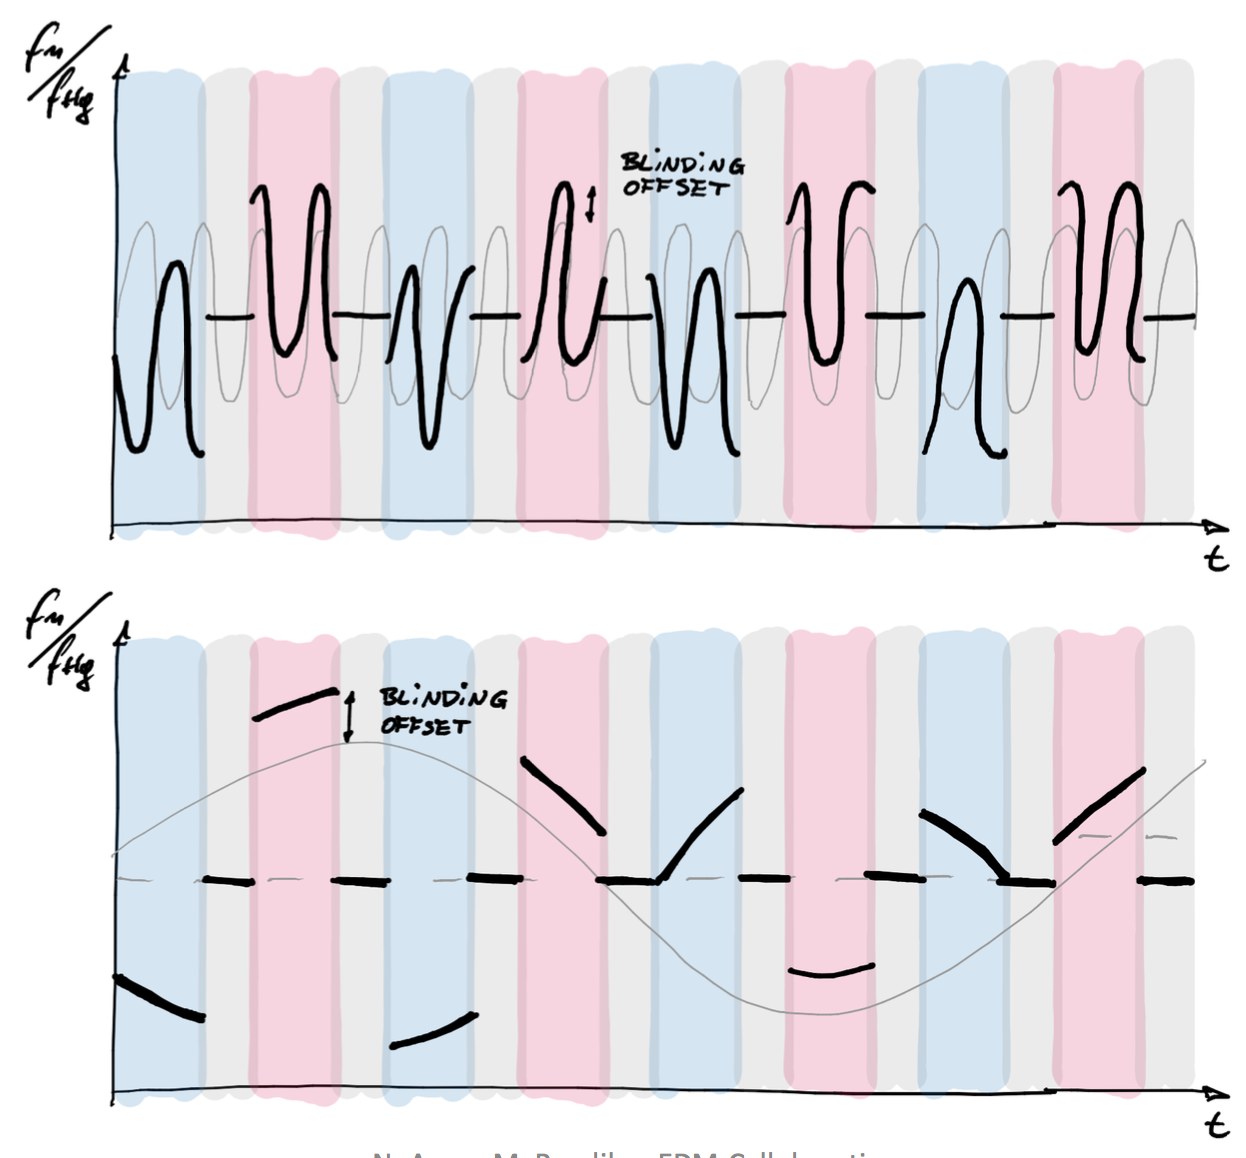
\includegraphics[width=\linewidth]{gfx/axions/cycle-level_blinding_offset.png}
  \caption{A sketch of how the blinding offset, and the true $d_n$, affect the $R$ time--series with a hypothetical axion--induced oscillation.}
  \label{fig:cycle-level_blinding_offset}
\end{figure}

The neutrons accumulate the phase during the free precession period. Therefore, the precession frequency that is measured is averaged over this period. In the Monte Carlo simulations it is assumed that the averaging occurs between the centres of the $\unit[2]{s}$ long spin--flip pulses, which is $\unit[202]{s}$.

\note{MR: How to combine the two data--sets? Gain in sensitivity only minor when using both. Maybe one can adjust for each hypothesis CL. 95\% -> $1 - \sqrt{0.05} = 0.78$, then something not seen in both on CL 78\% is exculded at 95\%. Would be tricky to implement exactly (the exclusion regions from the two datasets are not \emph{exactly} the same). What to do with the E=0 data--set? Cannot correct with it (checked that). Maybe just leave it as a check.}

The PSI data set uses, naturally, a different set of frequencies then the RAL--Sussex one. Due to the shorter time of data taking, the spectral resolution is lower (the inverse of $4.5$ months, $\unit[\sim 10^{-9}]{Hz}$), but denser sampling allows for going to higher frequencies. For the highest frequency we choose $\approx \unit[4 \cdot 10^{-3}]{Hz}$ \note{MR: still to be discussed}, which is a bit larger than the inverse separation of cycles. Then we choose the complete set of frequencies in an analogous way to the long time--base analysis, arriving at $\sim 10^6$ frequencies to analyse.

% \begin{figure}[htb]
% \begin{center}
% 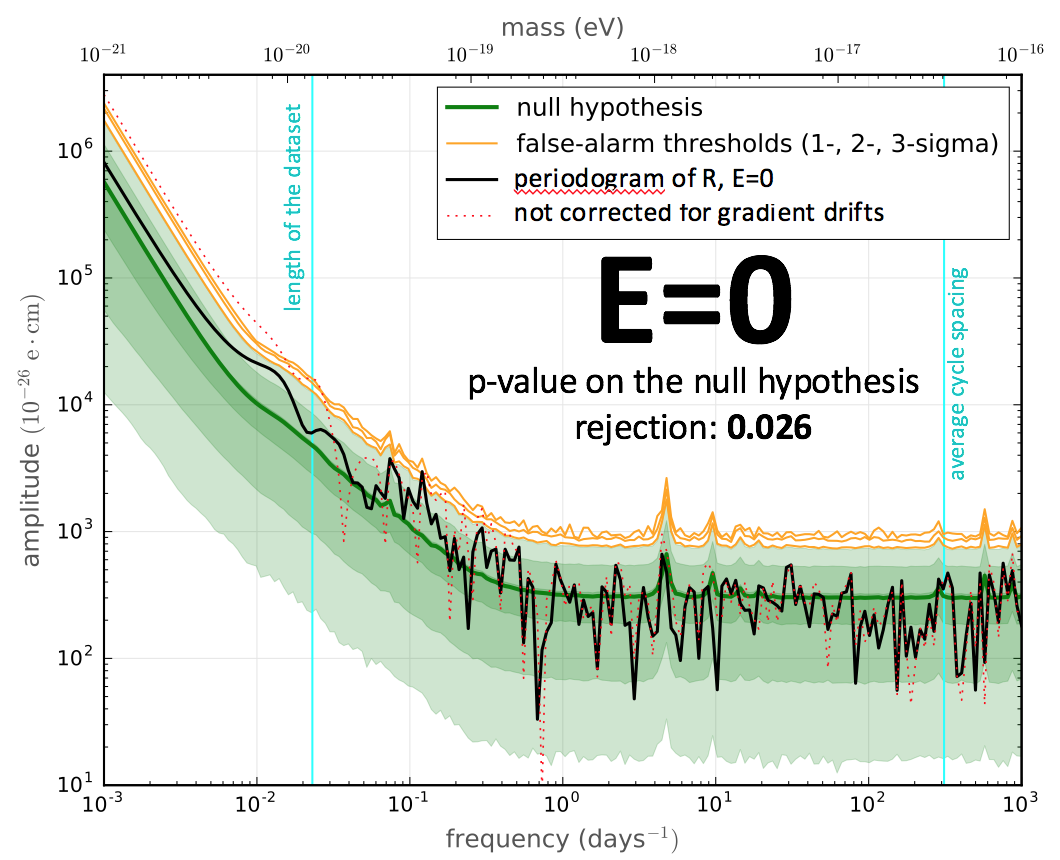
\includegraphics[width=0.5\columnwidth]{PSI_E0}
% 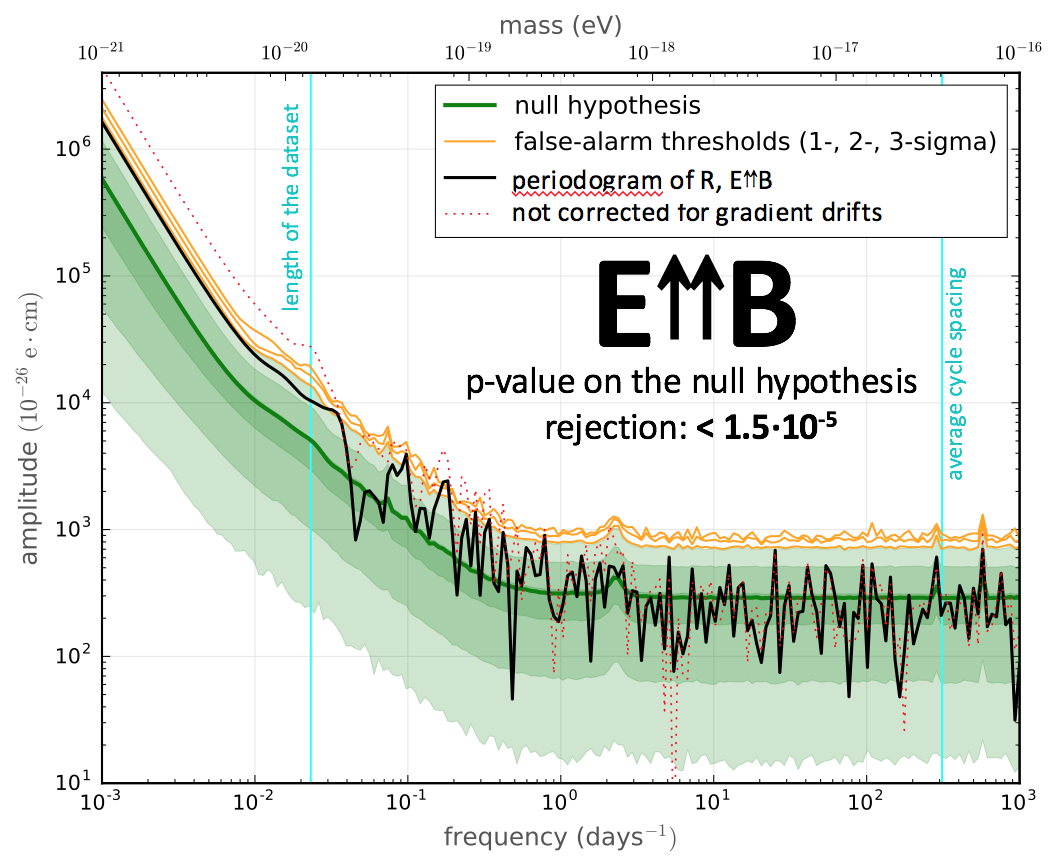
\includegraphics[width=0.5\columnwidth]{PSI_EpB}
% 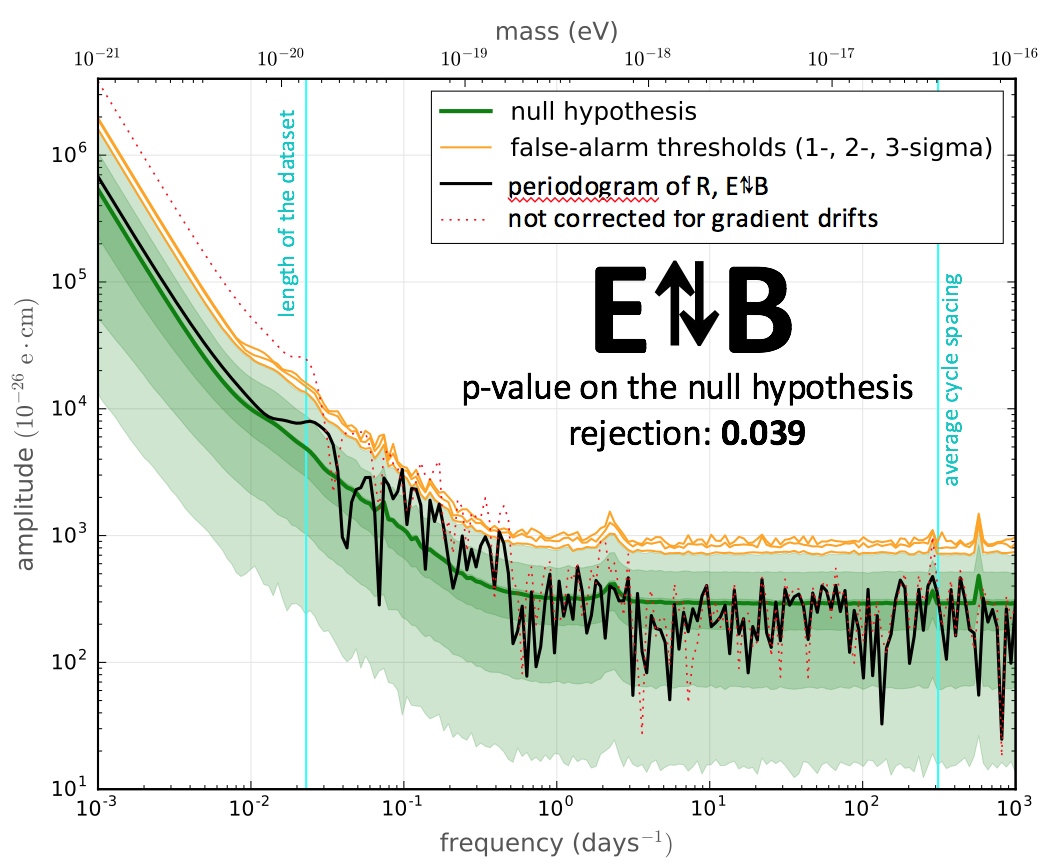
\includegraphics[width=0.5\columnwidth]{PSI_EapB}
% \caption{TODO \note{MR: The null hypothesis band is nearly identical for $E \neq 0$. Maybe plot only one and on top of that two periodograms of data? Also the plot is quite cluttered. Maybe plot only 95th percentile green line and 5\% false alarm threshold. Do NOT plot the bottom of distribution band -- it is meaningless, at least for our needs.}}
% \end{center}
% \end{figure}


\subsection{Systematic Studies for the Cycle--Level Analysis}
While the run--level analysis can benefit from all of the systematic studies done for the constant nEDM measurement, this is not the case for the lower level cycle--level analysis. An important decision has to be taken on how to treat the systematic effects. There are three options:
% \begin{enumerate}
%   \item Perform a detailed study of time--dependent systematic effect.
%   \item Determine \emph{delicate} frequencies and cut them out.
%   \item Assume there are no systematic effects.
% \end{enumerate}

\paragraph{Perform a detail study of time--dependent systematic effect.}
Here we would assume that any excess in power, in any dataset ($E \uparrow \uparrow B$, $E \uparrow \downarrow B$ and $E=0$) is a signature of some kind of a signal. All effects that can potentially result in that should be identified before the analysis is performed and corrected for. This would require a long and careful systematic study, a task much bigger then this analysis itself. Moreover, the full--fledged systematic studies for the constant nEDM analysis of the PSI data are still ongoing. Even though we acknowledge that this would be \emph{the} proper way to go, we consider it to be unrealistic and unnecessary for this analysis.

\paragraph{Determine \emph{delicate} frequencies and cut them out.}
Looking at periodograms of raw data one sees that there are several typical frequencies where peaks appear. Typically at inverse specific time constants at which the experiment operates: cycle separation, day, week, , HV--reversal, B0--reversal. We may decide that all systematic effects are constrained to these frequencies and do not perform the analysis there at all.

\paragraph{Assume there are no systematic effects.}
An axion would produce a very specific signal, in particular:
\begin{enumerate}
  \item There would be no signal in the $E=0$ dataset.
  \item The signal would appear in both $E~\uparrow~\uparrow~B$ and $E~\uparrow~\downarrow~B$ datasets, with equal amplitude.
  \item The signals in $E \uparrow \uparrow B$ and $E \uparrow \downarrow B$ would be shifted in phase by 180~degrees.
  \item The signals would have to have a high coherence of $\delta f / f = 10^{-6}$.
\end{enumerate}
In case we see an excess in power, we would only call it a candidate for an axion--signal if the three above conditions are met. Otherwise we attribute it to a, potentially unknown, systematic effect. We do realise the danger of making the systematic search dependent of the act of finding a signal. This automatically opens a line of attack on this analysis: we would not make a discovery, because a systematic effect has canceled the real signal out. We would not have seen a signal and therefore not looked for systematic effects. This is certainly valid. Nevertheless, we argue that the extremely low probability of this event, due to the high coherence of the axion field, makes it negligible. In order to cancel the axion signal, a systematic effect would not only need to be as coherent as the axion field, but additionally fine--tuned over at least 5 orders of magnitude magnitude of tested frequencies. With the coherence of $\delta f / f = 10^{-6}$ this is a tuning of $10^{-30}$. It would also need to be fine--tuned in amplitude over $\sim 20$ orders of magnitude, which gives a rough estimate of the cancellation probability: $10^{-50}$. As we are presenting limits with 95\% C.L., we feel this approach is justified.

Out of the three, we opt for the third option, but leave the subject open to discussion for the collaboration.


\subsection{Results of the short time--base analysis}
At the moment only a $\approx 40$ days long subset of the PSI data set has been analysed. The full data set will be analysed when the analysis method has been exactly established.

The results of the null hypothesis tests are presented in Fig.\,\ref{fig:cycle-level_detection}. Even though the data taking is not strictly synchronous throughout the whole data taking period, it is highly regular. This causes structures visible in the distributions of the null hypothesis periodograms. There is a sharp peak at the inverse median of the data points (cycles of the experiment), equal to $\unit[301]{s}$. The broader peaks at approximately inverse 10~hours in $E \neq 0$ and 5~hours in $E = 0$ datasets correspond to the periodicity of electric field changes in the apparatus. The electric field is changed according to the pattern: 8 cycles of no field, 48 in one direction, 8 of zero, 48 in the other direction. Thanks to the Monte Carlo simulations, the structures in the periodograms are reproduced and accounted for in the hypotheses testing.

The global p-values for the $E=0$ and $E \uparrow \downarrow B$ are 0.53 and 0.12 respectively, indicating agreement with the null hypothesis. The global p-value for the $E \uparrow \uparrow B$ dataset is $3.4 \cdot 10^{-5}$, which is on the 4--sigma level. However, the corresponding frequency is in the delicate region around the inverse median spacing of data points. As the peak does not appear in the $E \uparrow \downarrow B$ dataset, and the 5--sigma threshold has not been crossed, we do do not consider it to be an indication of an axion signal.


\begin{figure}[h!]
  \centering 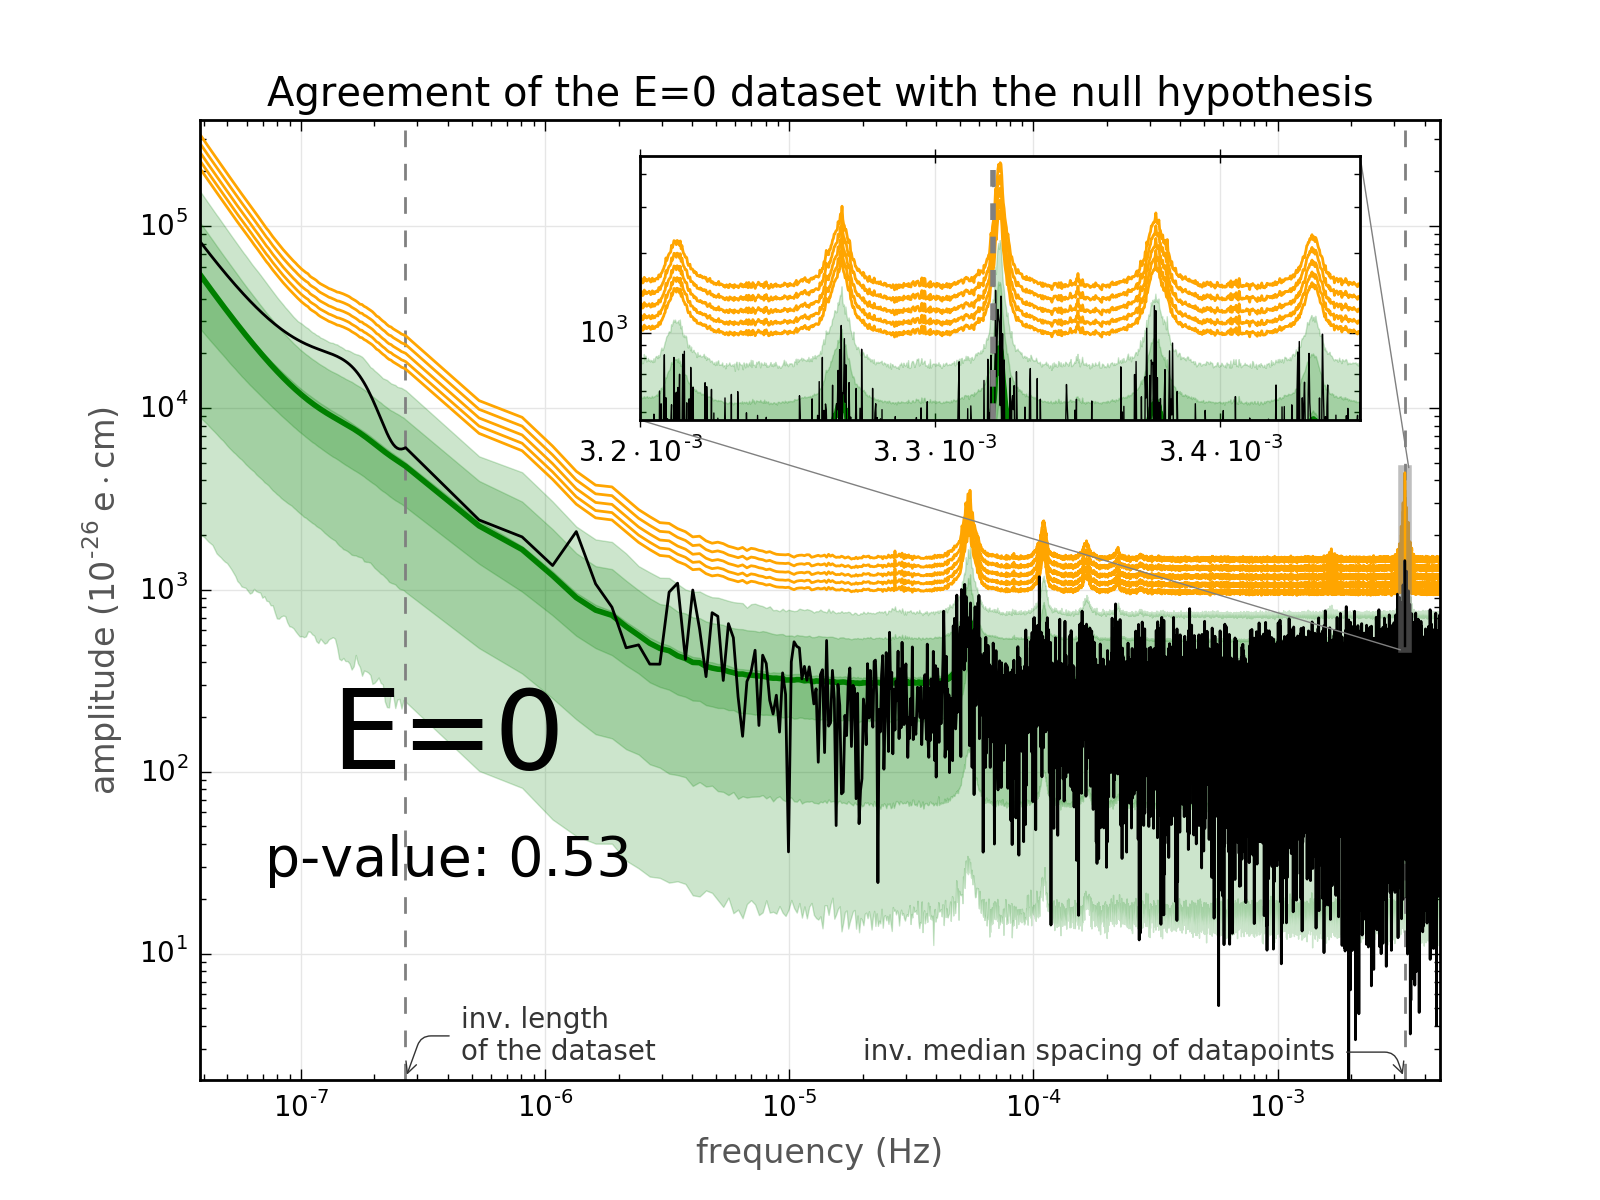
\includegraphics[width=0.9\linewidth]{gfx/axions/cycle-level_E0_detection.png}
  \centering \includegraphics[width=0.9\linewidth]{gfx/axions/cycle-level_EBp_detection.png}
  \centering \includegraphics[width=0.9\linewidth]{gfx/axions/cycle-level_EBap_detection.png}
  \label{fig:cycle-level_detection}
  \caption{Results of the three datasets ($E=0$, $E \uparrow \uparrow B$, $E \uparrow \downarrow B$) compatibility with the null hypothesis tests. The two--dimensional distribution of the null hypothesis periodogram is depicted with green bands, thick green line being the mean. The orange lines depict 1-, 2-, 3-, 4- and 5-sigma false--alarm thresholds. The inverse length of the dataset and inverse median spacing of the datapoints are marked with dashed vertical lines. The structures visible in the distribution of the null hypothesis periodogram are solely due to the time scheme of data taking. High correlation for frequencies lower then the inverse length of the dataset is visible even with bare eye. This is expected, as those frequencies are separated by less then the spectral resolution of the data set.}
\end{figure}

% \begin{figure}[htb]
%   \centering 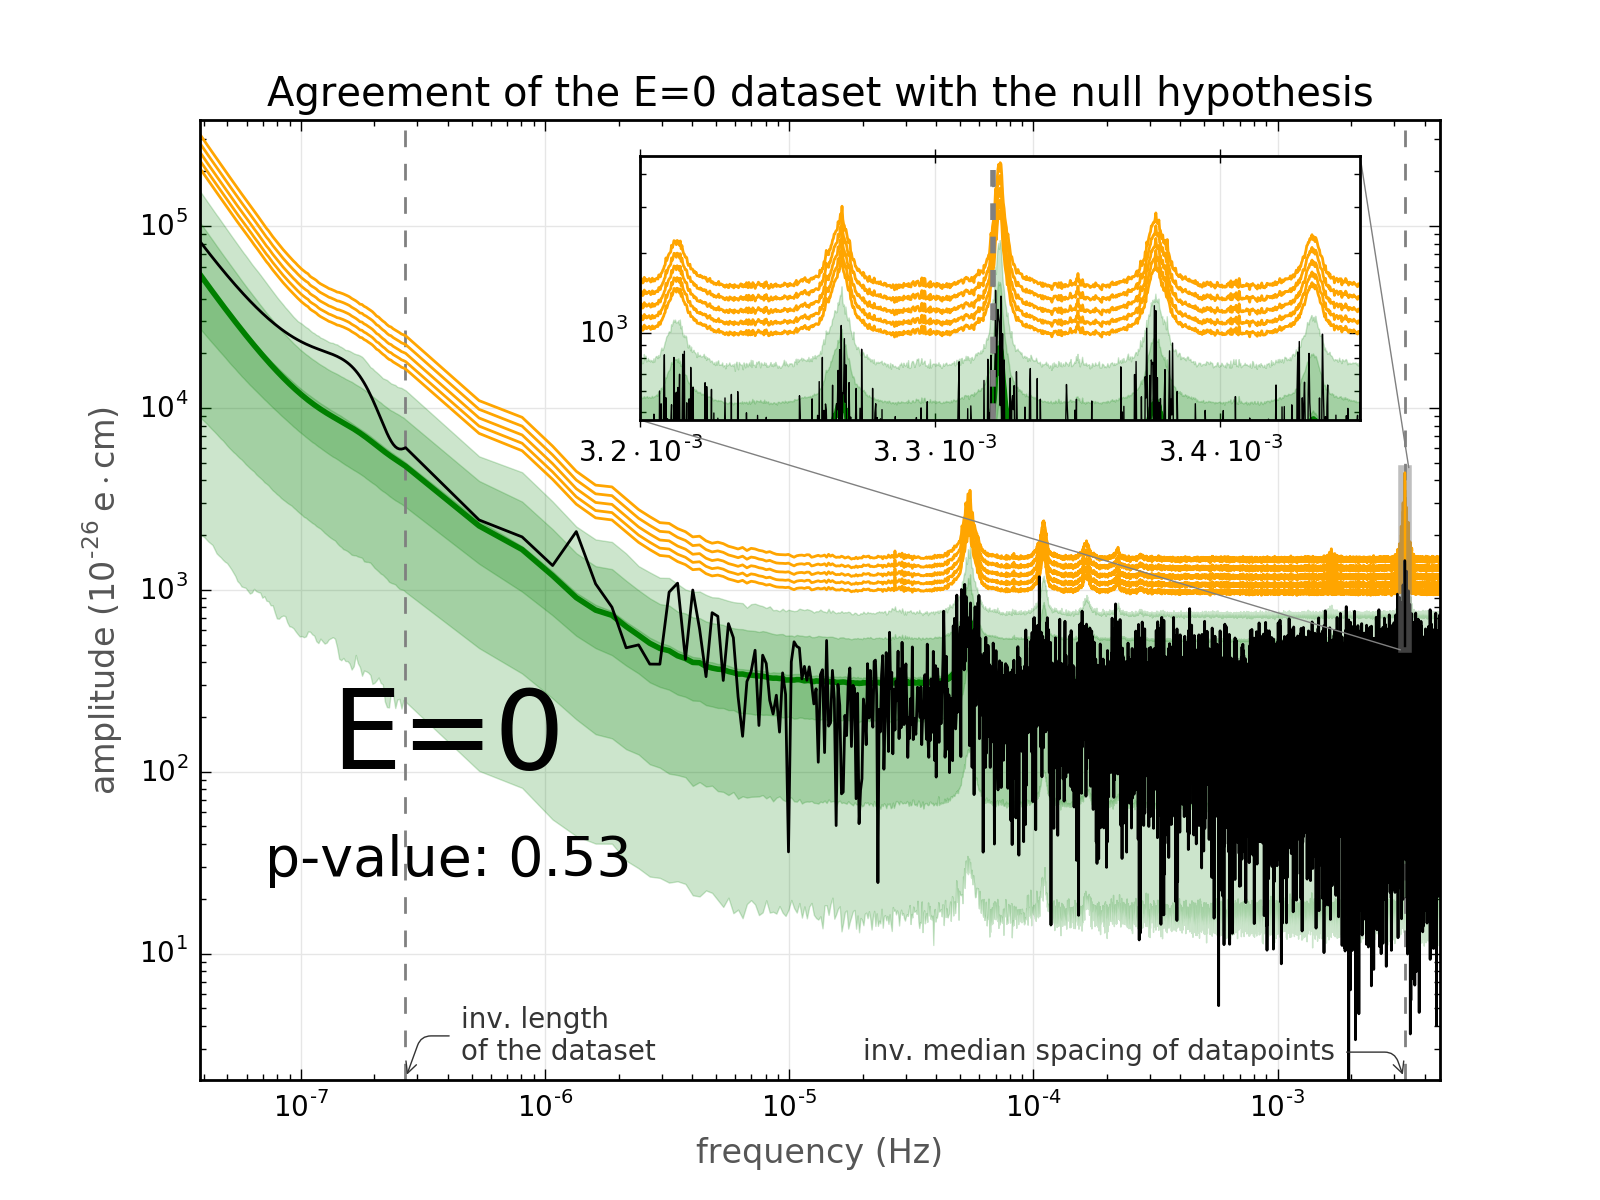
\includegraphics[width=\linewidth]{gfx/axions/cycle-level_E0_detection.png}
%   \caption{Results of the test dataset ($E=0$) compatibility with the null hypothesis. The two--dimensional distribution of the null hypothesis periodogram is depicted with green bands, thick green line being the mean. The orange lines depict 1-, 2-, 3-, 4- and 5-sigma false--alarm thresholds. The inverse of the length of the dataset and of the median spacing of the datapoints are marked with dashed vertical lines. The structures visible in the distribution of the null hypothesis periodogram are solely due to the time structure of how the data was taken.}
%   \label{fig:cycle-level_E0_detection}
% \end{figure}
%
% \begin{figure}[htb]
%   \centering \includegraphics[width=\linewidth]{gfx/cycle-level_EBp_detection.png}
%   \caption{\note{MR: TODO The very low p-value is due to a peak (on a 4--sigma level) which is very close to the inverse median spacing of datapoints. Need to investigate. Will it appear in EBap dataset too?}}
%   \label{fig:cycle-level_EBp_detection}
% \end{figure}
%
% \begin{figure}[htb]
%   \centering \includegraphics[width=\linewidth]{gfx/cycle-level_EBap_detection.png}
%   \caption{\note{MR: TODO}}
%   \label{fig:cycle-level_EBap_detection}
% \end{figure}

The exclusion regions obtained from the two $E \neq 0$ datasets are shown in Fig.\,\ref{fig:cycle-level_exclusion}.

\begin{figure}[htb]
  \centering 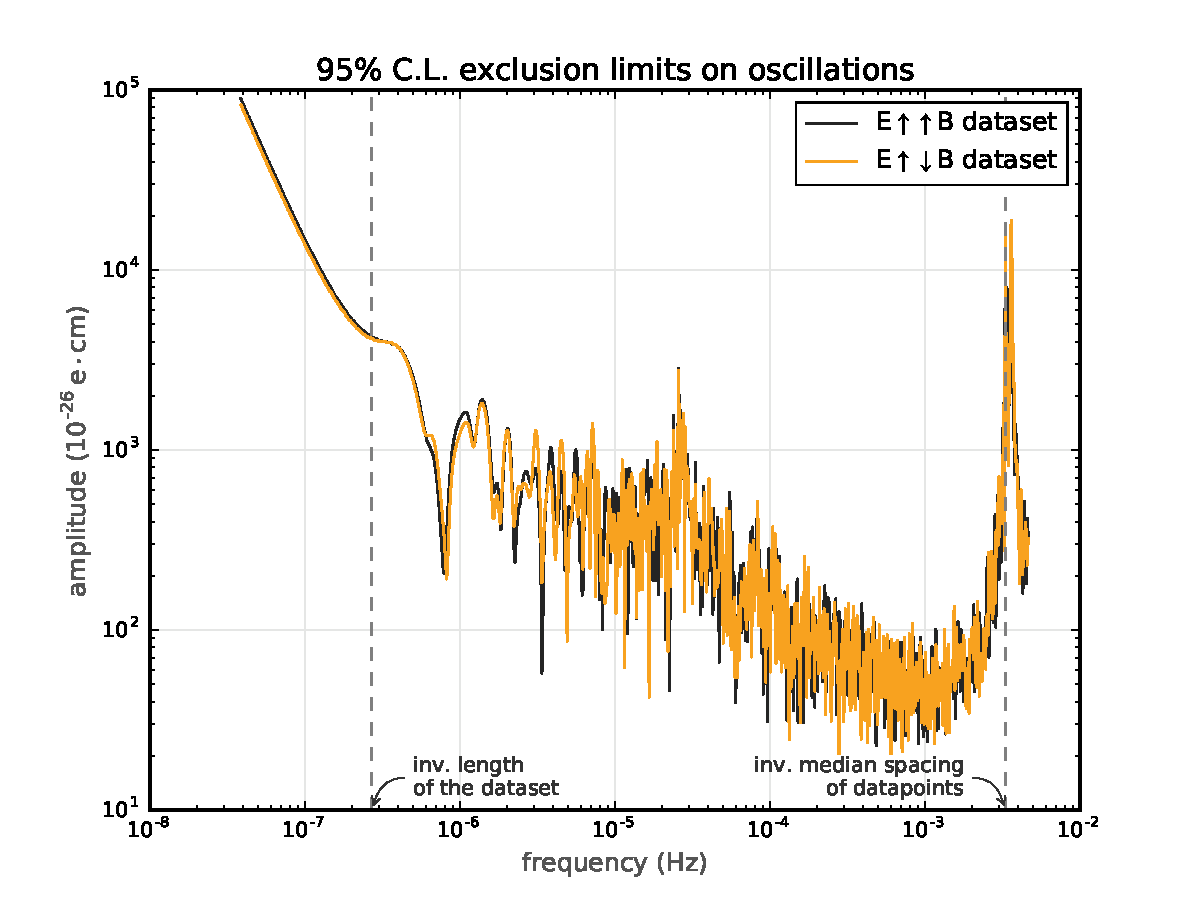
\includegraphics[width=\linewidth]{gfx/axions/cycle-level_exclusion_bisection.pdf}
  \caption{Exclusion regions obtained with the $E \uparrow \uparrow B$ and $E \uparrow \downarrow B$ datasets. Excluded are amplitudes higher then the line drawn. The regions for the two datasets are nearly identical, as expected. For periods longer then the length of the dataset a rapid loss of sensitivity is observed. Also, sensitivity to exclusion is significantly worse in the region around the inverse median spacing of the datapoints (equal to the cycling frequency of the experiment).}
  \label{fig:cycle-level_exclusion}
\end{figure}



%%%%%%%%%%
\section{Results in the axion context}


\note{Present results (including graphs) for axion-gluon coupling, and $g_d$ effective coupling (to compare with CASPEr notation)?, axion-neutron coupling, axion-proton coupling, axion-electron coupling?}






%%%%%%%%%%
\textbf{Conclusions.} ---
















%%%%%%%%
%\section*{ACKNOWLEDGEMENTS}
\textbf{Acknowledgements.} ---
\note{We are grateful to Maxim Pospelov and Edward Witten for helpful discussions. This work was supported by .... }

%the Australian Research Council.
%the Royal Astronomical Society.



%%%%%%%%%
%\section*{Appendix}
\appendix

%%%%%%%%%%
\textbf{Appendix A:~Summary of Existing Constraints.} ---
Here we summarise the existing constraints on the axion mass and interaction parameters in Eq.~(\ref{Axion_couplings}) from laboratory searches and measurements pertaining to astrophysics and cosmology.

\begin{figure}[h!]
  \begin{center}
  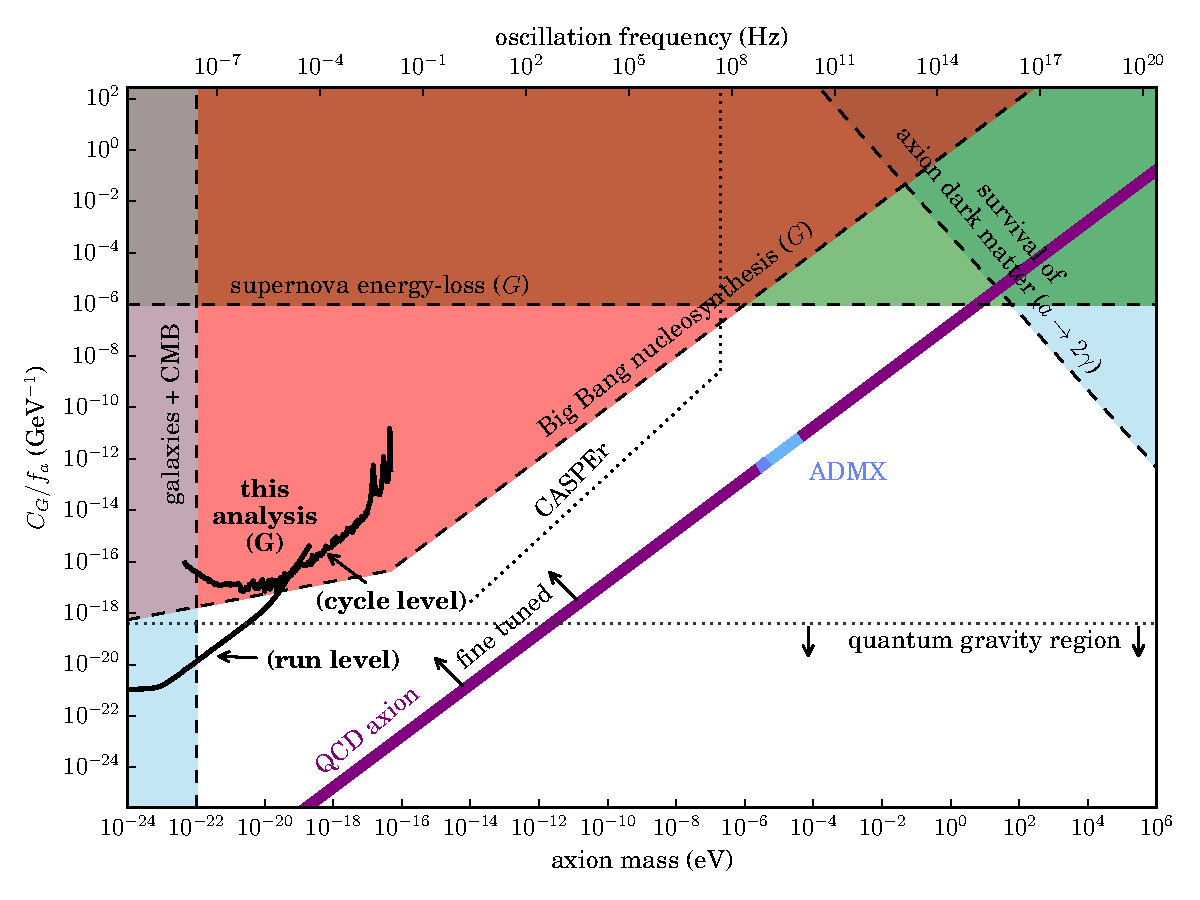
\includegraphics[width=\columnwidth]{gfx/axions/axion_limits_only_G}
  \caption{Our exclusion limits in the axion landscape. \note{MR: The limits plotted on this figure are slightly outdated. The cycle level includes only a subset of data. I think we should include a plot with limits on the nEDM oscillation itself (nEDM in 1e-26 ecm vs frequency). This is potentially of interest to a wider community. Also need to carefully decide which other limits to include on the plot.}}
  \end{center}
\end{figure}

An upper limit on the mass of axions, which saturate the observed cold DM content and form an oscillating classical field, is set by the requirement that there are a large number of axions within the reduced de Broglie volume (i.e., $n_a \left( \lambda_{\textrm{dB}}/2\pi \right)^3 \gg 1$):~$m_a \lesssim 0.1$ eV.
Sufficiently low-mass and feebly-interacting axions can survive to the present day.
For the QCD axion, this requires $m_a \lesssim 24$ eV in order for the $a \to 2 \gamma$ decay channel to be sufficiently suppressed, while for more generic ALPs, the restriction is generally less severe, meaning that the upper mass bound $m_a \lesssim 0.1$ eV is readily satisfied (see, e.g., \cite{Fields2015ALP_decay}).
For $m_a \gtrsim 0.1$ eV, axions may contribute to hot DM (see, e.g., \cite{Archidiacono2013_hot_axion_DM}).

The simplest lower limit on the mass of axions, which saturate the observed cold DM content, comes from the requirement that their de Broglie wavelength not exceed the DM halo size of the smallest dwarf galaxies ($R \sim 1$ kpc):~$m_a \gtrsim 10^{-22}$ eV.
Ultra-low-mass axion DM only behaves like perfect cold DM on length scales larger than the axion de Broglie wavelength.
On shorter length scales, their gravitational collapse is prevented by the gradient energy in the axion field \cite{Khlopov1985}.
This characteristic feature of ultra-low-mass axion DM has non-trivial consequences for cosmology.
In particular, if axions saturate the observed DM content, then existing CMB measurements require $m_a \gtrsim 10^{-24}$ eV \cite{Marsh2015A}, while consistency with observed structure formation requires $m_a \gtrsim 10^{-22}$ eV \cite{Marsh2015B,Schive2015}.

Due to its effects on structure formation, ultra-low-mass axion DM in the mass range $10^{-24}~\textrm{eV} \lesssim m_a  \lesssim 10^{-20}$ eV has been proposed to resolve several long-standing ``small-scale crises'' of the cold DM model \cite{Hu2000,Marsh2014,Paredes2015}.
In the future, cosmological observations may be able to distinguish ultra-low-mass axion DM with masses $m_a \lesssim 10^{-18}~\textrm{eV}$ from standard cold DM \cite{Marsh2015C}. Gravitational wave astronomy \cite{LIGO2016} has the potential to discover signals due to black hole superradiance caused by axions in the mass range $10^{-18}~\textrm{eV} \lesssim m_a  \lesssim 10^{-12}$ eV \cite{Marsh2015Review,Arvanitaki2010}.

The most stringent astrophysical limits on the axion-gluon coupling for the axion masses of interest in the present work come from Big Bang nucleosynthesis (BBN).
At second order, the axion-gluon coupling in Eq.~(\ref{Axion_couplings}) increases the neutron-proton mass difference via the effective operator $\mathcal{L}_{\textrm{eff}} = (f_\pi \bar{g}^{(0)}_{\pi N N} / 2) (m_d - m_u)/ (m_d + m_u) (C_G a / f_a)^2 \bar{N} \tau^3 N$:~$\delta Q_{np} \approx 0.37~\textrm{MeV}~\left(C_G a / f_a \right)^2$ \cite{Ubaldi2010,Blum2014}, altering the primordial abundances of light elements produced during BBN.
Comparison of measurements and SM calculations of the primordial $^4$He abundance gives the following rough constraints \cite{Blum2014}:
\begin{eqnarray}
\label{aGG_BBN_limits}
\frac{m_a^{1/4} f_a}{ C_G} \gtrsim 10^{10}~\textrm{GeV}^{5/4}, ~ \textrm{$m_a \ll 10^{-16}$ eV },\\
\frac{m_a f_a}{ C_G} \gtrsim 10^{-9}~\textrm{GeV}^2, ~ \textrm{$m_a \gg 10^{-16}$ eV },
\end{eqnarray}
assuming that axions saturate the present-day DM content.
The axion-gluon coupling also induces the following effective operator via the process shown in Fig.~1a:~$\mathcal{L}_{\textrm{eff}} = (-i g^d_N / 2) a \bar{N} \sigma_{\mu \nu} \gamma_5 N F^{\mu \nu}$, with $g^d_n \approx (2.4 \times 10^{-16} C_G / f_a) ~ e \cdot \textrm{cm} = (3.7 \times 10^{-3} C_G / f_a) ~\textrm{GeV}^{-1}$ and $g^d_n \simeq - g^d_p$.
Applying supernova energy-loss bound arguments to this effective operator for the process $N + \gamma \to N + a$ give the following rough constraint \cite{Graham2013}:
\begin{equation}
\label{aGG_SN_limits}
\frac{f_a}{C_G} \gtrsim 10^6 ~\textrm{GeV}, ~ \textrm{$m_a \lesssim 3 \times 10^{7}$ eV} \, ,
\end{equation}
which is significantly weaker than the above BBN constraints for the mass range of interest in the present work.


The most stringent astrophysical limits on the axion-nucleon couplings come from supernova energy-loss bound arguments applied to the bremsstrahlung channel $N + N \to N + N + a$, which give the rough constraint (see \cite{Raffelt2008LNP} and the references therein):
\begin{equation}
\label{aNN_SN_limits}
\frac{f_a}{C_N} \gtrsim 10^9 ~\textrm{GeV}, ~\textrm{$m_a \lesssim 3\times 10^{7}$ eV} \, .
\end{equation}
The most stringent laboratory limits on the axion-neutron coupling come from a K$/^{3}$He co-magnetometry search for new spin-dependent forces mediated by virtual axion exchange \cite{Romalis2009_NF}:
\begin{equation}
\label{ann_lab_limits}
\frac{f_a}{C_n} > 1 \times 10^4 ~\textrm{GeV}, ~\textrm{$m_a \lesssim 10^{-7}$ eV} \, ,
\end{equation}
while the most stringent laboratory limits on the axion-proton coupling come from a H$_{2}$ spectroscopy search for analogous new spin-dependent forces \cite{Romalis2009_NF,Ramsey1979}:
\begin{equation}
\label{app_lab_limits}
\frac{f_a}{C_p} > 60 ~\textrm{GeV}, ~\textrm{$m_a \lesssim 10^{5}$ eV}  \, .
\end{equation}


The most stringent astrophysical limits on the axion-electron coupling come white dwarf cooling arguments applied to the bremsstrahlung channel $e^{-} + (Z,A) \to e^{-} + (Z,A) + a$, which give the rough constraint (see \cite{Raffelt2008LNP} and the references therein):
\begin{equation}
\label{aee_WD_limits}
\frac{f_a}{C_e} \gtrsim 10^{10} ~\textrm{GeV}, ~\textrm{$m_a \lesssim 10^3$ eV} \, .
\end{equation}
The most stringent laboratory limits on the axion-electron coupling come from a rotating torsion pendulum search for new spin-dependent forces mediated by virtual axion exchange \cite{Adelberger2013}:
\begin{equation}
\label{aee_lab_limits}
\frac{f_a}{C_e} > 3 \times 10^4 ~\textrm{GeV}, ~\textrm{$m_a \lesssim 10^{-7}$ eV} \, .
\end{equation}


%%%%%%%%%%%
\textbf{Appendix B:~Model for Ultra-low-mass Axions with $C_G\sim 1$.} ---
Here we sketch a model, for which $C_G\sim 1$, but which also satisfies $m_af_a\ll C_G\Lambda_{\mathrm{QCD}}^2$. Ref.~\cite{Blum2014} showed that such a model could not be achieved via the mass mixing of two axions coupled to the QCD sector, with an additional UV mass source.
Our model, on the other hand, has a single axion with two non-perturbative sources of mass. Consider the following Lagrangian (note that we supress the index summation here):
\begin{equation}
\label{Hidden-QCD_L}
\mathcal{L}\supset \frac{C_G}{f_a}\frac{g}{32 \pi^2}a G\tilde{G}+\frac{C_X}{f_a}\frac{g_X}{32 \pi^2}a X\tilde{X} \, ,
\end{equation}
where $X$ is the gauge field strength of some confining, non-Abelian, CP-violating hidden sector.
The gauge coupling is $g_X$, and the hidden-sector quarks that are charged in $X$ give rise to a $C_X$-anomaly under the Peccei-Quinn symmetry.

The first term in Eq.~(\ref{Hidden-QCD_L}) gives rise to the usual axion potential due to QCD instantons.
Since QCD is CP-conserving in the absence of instantons, this potential is minimised at $a=0$ \cite{Vafa1984}.
The potential due to instantons in $X$, however, will be minimised at some other value, in general causing CP violation.
Consider the following axion potential at low energies when the QCD sector and the hidden sector are both in the confining phase:
\begin{align}
V(a) &= \Lambda_{\mathrm{QCD}}^4 \left[1- \cos \left(\frac{C_G a}{f_a}\right) \right] \notag \\
&+ \Lambda_{\mathrm{X}}^4 \left[1- \cos \left(\frac{C_X a}{f_a} + \delta \right)\right] \, ,
\end{align}
where $\Lambda_{\mathrm{QCD}} \approx 250$ MeV is the QCD scale and $\Lambda_X$ is the strong coupling scale of the hidden sector.
If the hidden sector strongly violates the CP symmetry, then one can have $\delta=\pi$, %{\color{red} what is the case for SU(2)?}
in which case the axion mass around the $a=0$ vacuum is given by:
\begin{equation}
m_a^2 = m_{\mathrm{QCD}}^2 (1-r^4) \, .
\end{equation}
where $m_{\mathrm{QCD}} = C_G\Lambda_{\mathrm{QCD}}^2/f_a$ and $r=(\Lambda_X C_X^{1/2})/(\Lambda_{\mathrm{QCD}}C_G^{1/2})$.
With sufficient fine-tuning of the ratio $r$, it is possible to construct a model with an ultra-low-mass axion, which produces a significantly larger oscillating neutron EDM and significantly larger oscillating atomic EDMs (generated via hadronic mechanisms), compared with the QCD axion.
If $r^4<1$ and $\delta=\pi$, the minimum of the potential exactly conserves the CP symmetry, leading to EDMs that oscillate about zero at a low frequency.
If $r^4>1$, and/or if $0<\delta<\pi$, the potential violates the CP symmetry, and an EDM oscillates about a non-zero value.

The fine-tuning in this model is related to the fine-tuning that defines the strong CP problem, i.e., a cancellation between CP-violating effects in different non-Abelian sectors.
This model is not intended to solve the strong CP problem, but to provide a setting in which the $\theta_{\textrm{QCD}}$ angle of QCD oscillates with a low frequency.
An observation of a low-frequency oscillating EDM of the neutron would present a fine-tuning problem for axion models.




\textbf{Appendix C:~Validation of analysis techniques and code} ---

The analysis of the ILL and PSI datasets was performed by two separate codes, with the ILL code written mostly by Nick in Python and the PSI code written mostly by Michał in Julia. None of the code used for calculations is shared between the programs or based on the code of the other program. However, both codes do implement the same analysis technique.

We want to ensure two things:
\begin{itemize}
\item {The codes are implementing the algorithms correctly}
\item {The algorithms are correct to give good results}
\end{itemize}

To accomplish the first objective we analyse the same datasets using both the ILL and PSI codes. To accomplish the second we compare some of the results of the simpler ILL analysis to analytical predictions where these exist.

\textbf{Appendix D:~How we determined how many Monte-Carlo samples were needed}

\section{Comparison of the two analyses}
\label{Sec:comparison}
The two analyses, long and short time--base, were developed as two separate codes. First by Nicholas Ayres, second by Michal Rawlik. However, the mathematical foundation of both is the same and it is, therefore, expected that the two implementations, given the same input, should give the same results.

Nine fake time series (\emph{datasets}) have been generated. For each dataset a set of frequencies to analyse has been agreed on. The long time--base analysis has been modifed to fit a constant offset in the LSSA fits. For each dataset we compare the \emph{detection} analysis and determination of the exclusion region in the signal space. The comparison in the detection analysis is presented in Fig.\,\ref{fig:comparison_detection}, where we compare:
\begin{enumerate}
  \item The periodogram of the dataset --- here we observe an agreement on  the $10^{-6}$ level.
  \item The average periodogram for the null hypothesis --- here we observe a 40\% disagreement for the lowest tested frequency. For all other frequencies the agreement is better then 4\% and is clearly dominated by numerical noise (which can be decreased by using more Monte Carlo samples.)
  \item The 1-, 2-, 3-, 4- and 5-sigma false--alarm thresholds --- we observe the same situation as for the average periodogram for the null hypothesis.
\end{enumerate}
For the exclusion region determination we compare the p--value on the signal hypothesis exclusion on a space spanned by frequency and amplitude of the signal. The comparison is presented in Fig.\,\ref{fig:comparison_exclusion}. In most interesting region, the boundary between the black and white areas, we observe differences on the order of few per cent. Because the differences are not systematic, they are most likely caused by numeric noise.

\begin{figure*}[ptb]
  \centering 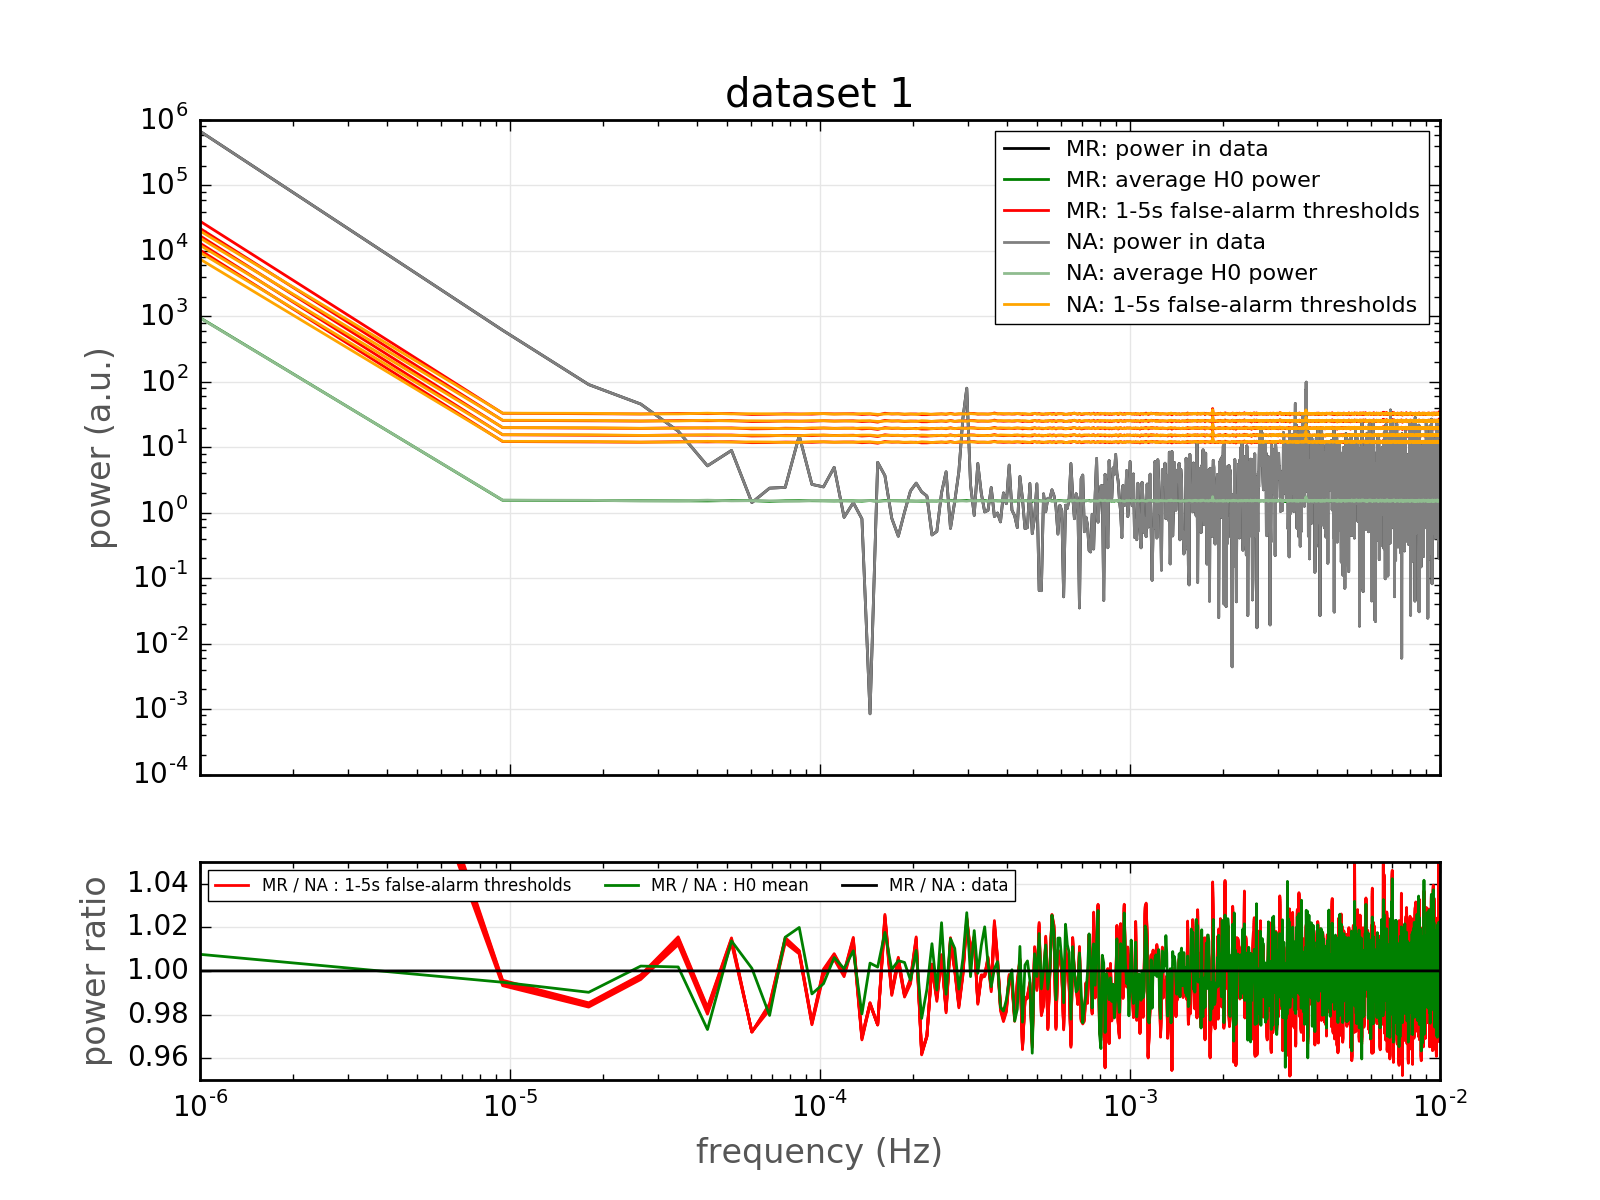
\includegraphics[width=0.32\linewidth]{gfx/axions/comparison/comparison_detection_dataset1.png}
  \centering 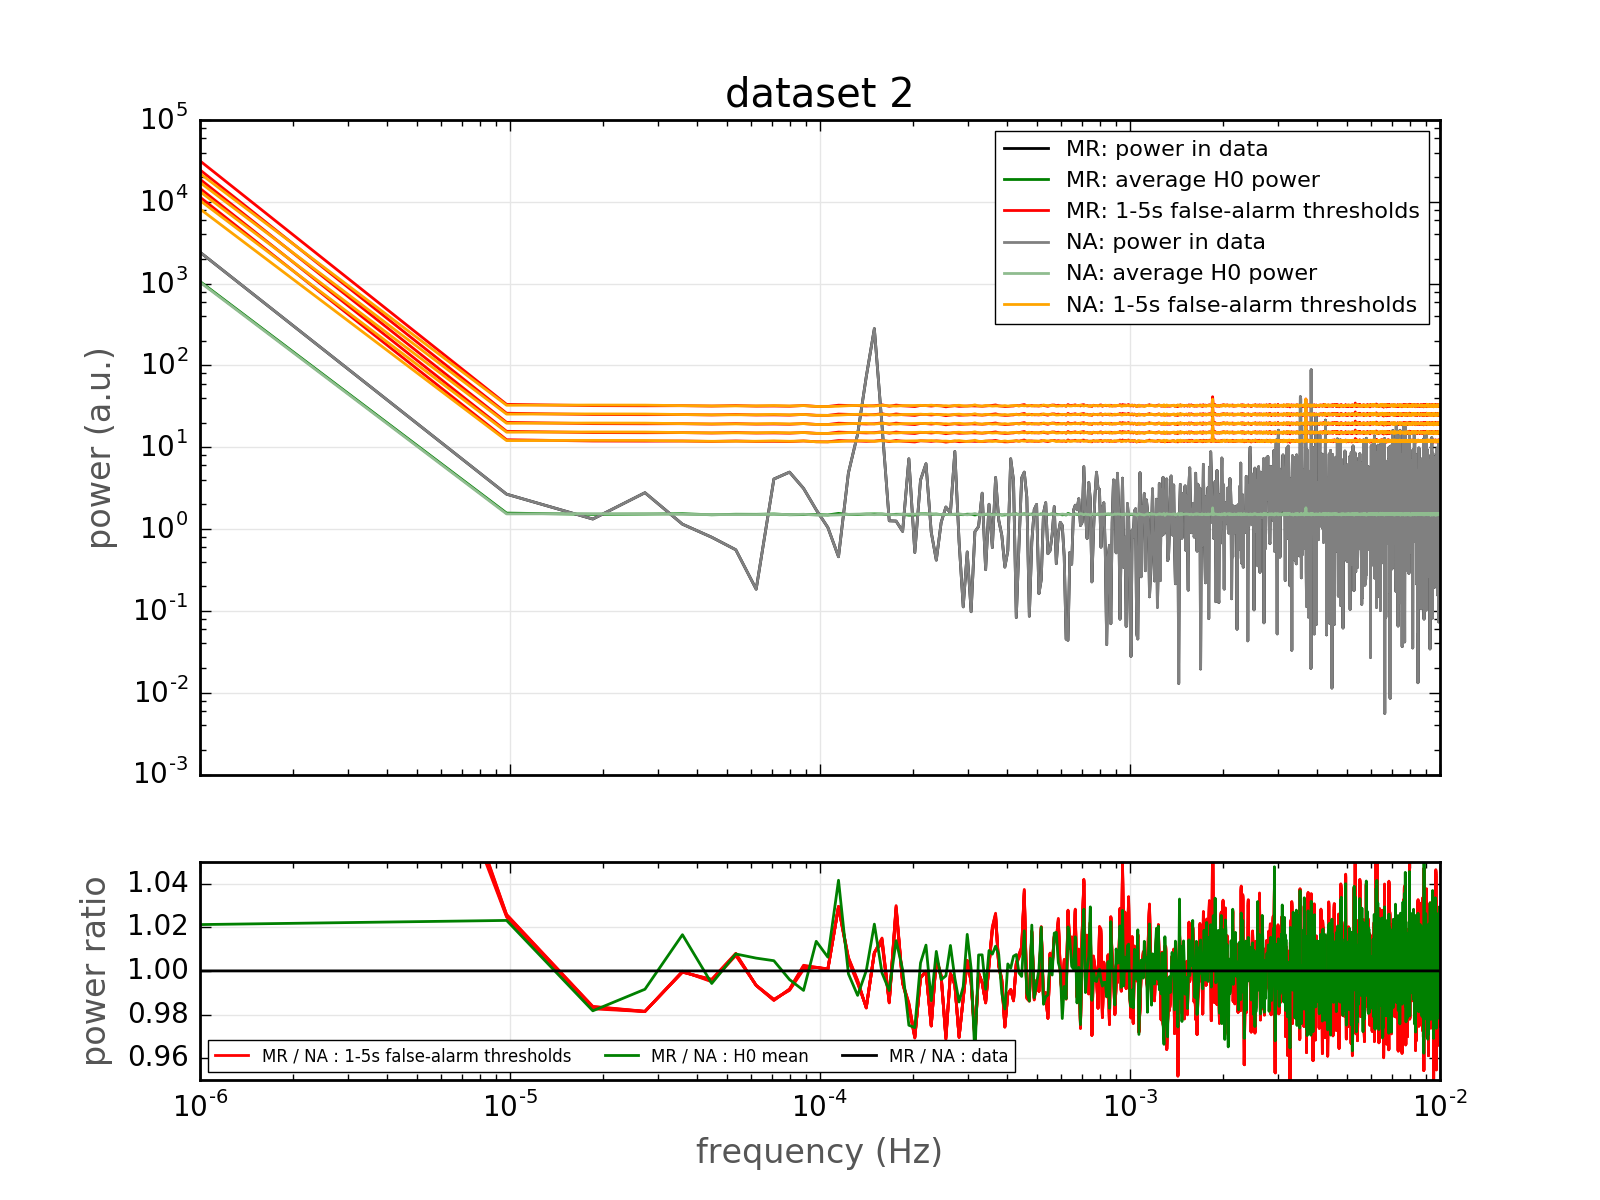
\includegraphics[width=0.32\linewidth]{gfx/axions/comparison/comparison_detection_dataset2.png}
  \centering 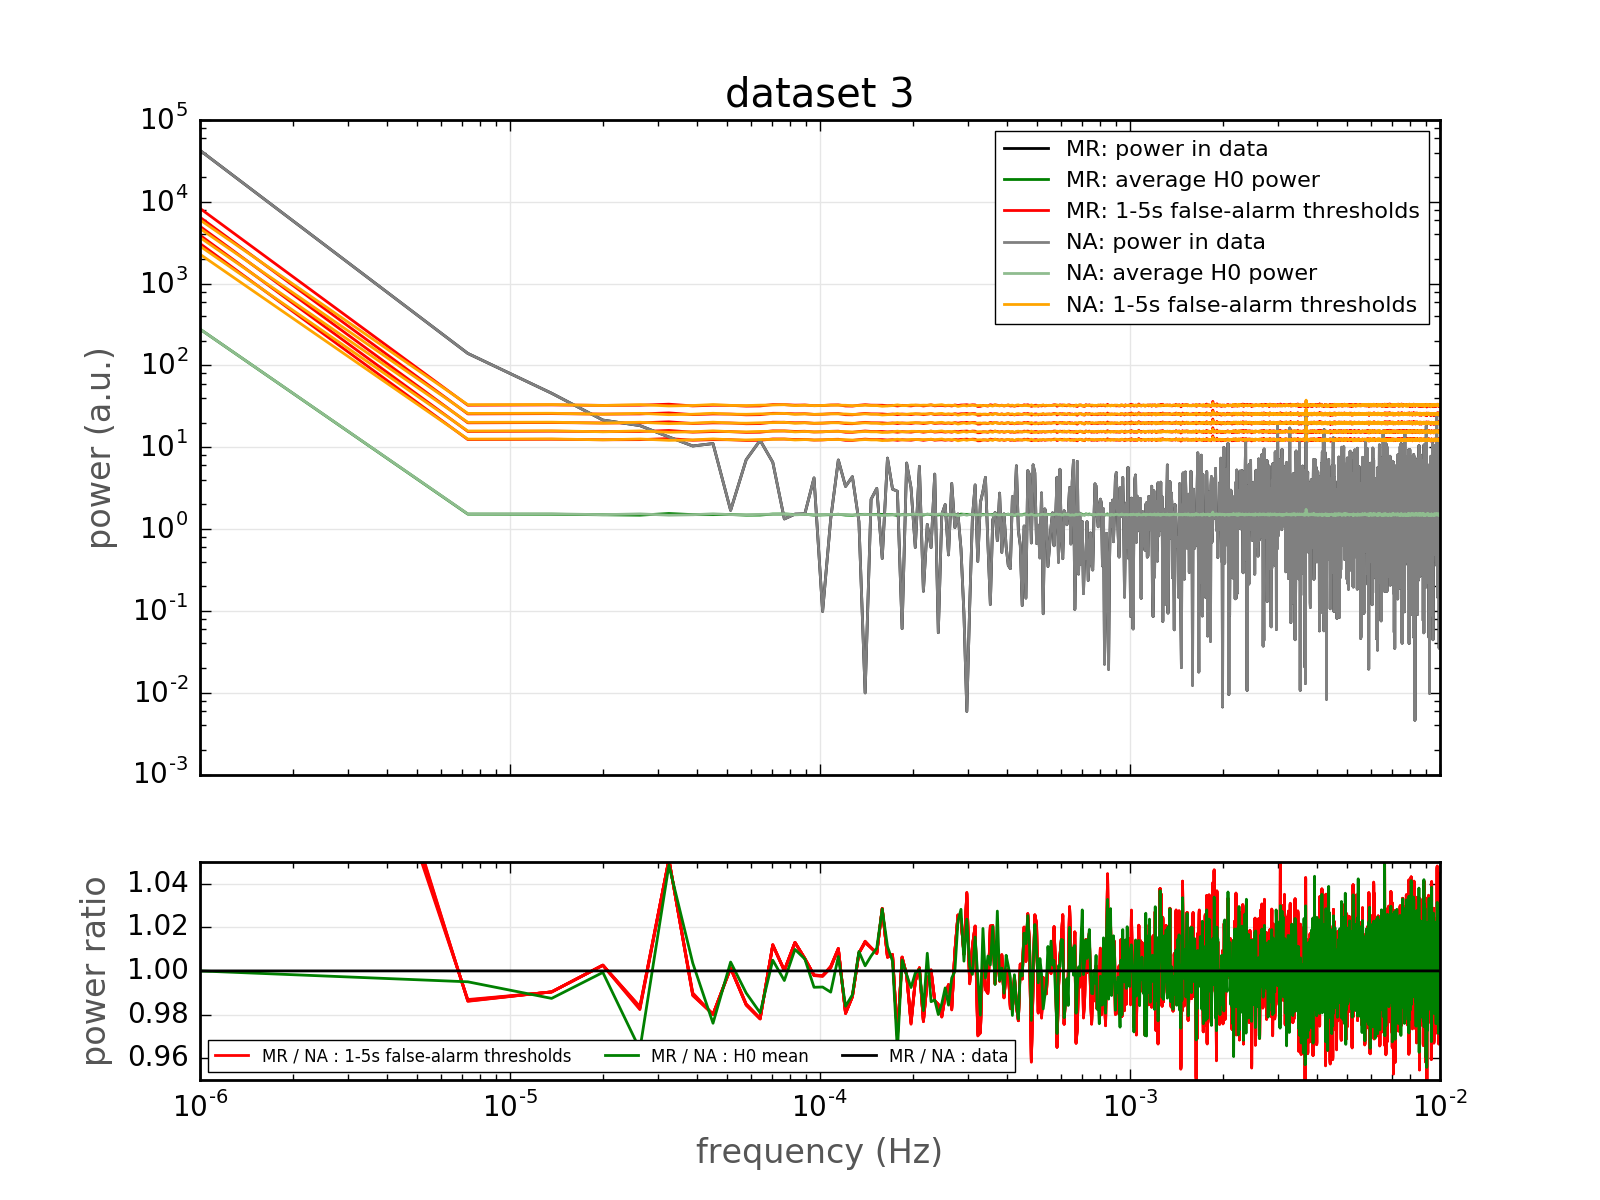
\includegraphics[width=0.32\linewidth]{gfx/axions/comparison/comparison_detection_dataset3.png}
  \centering 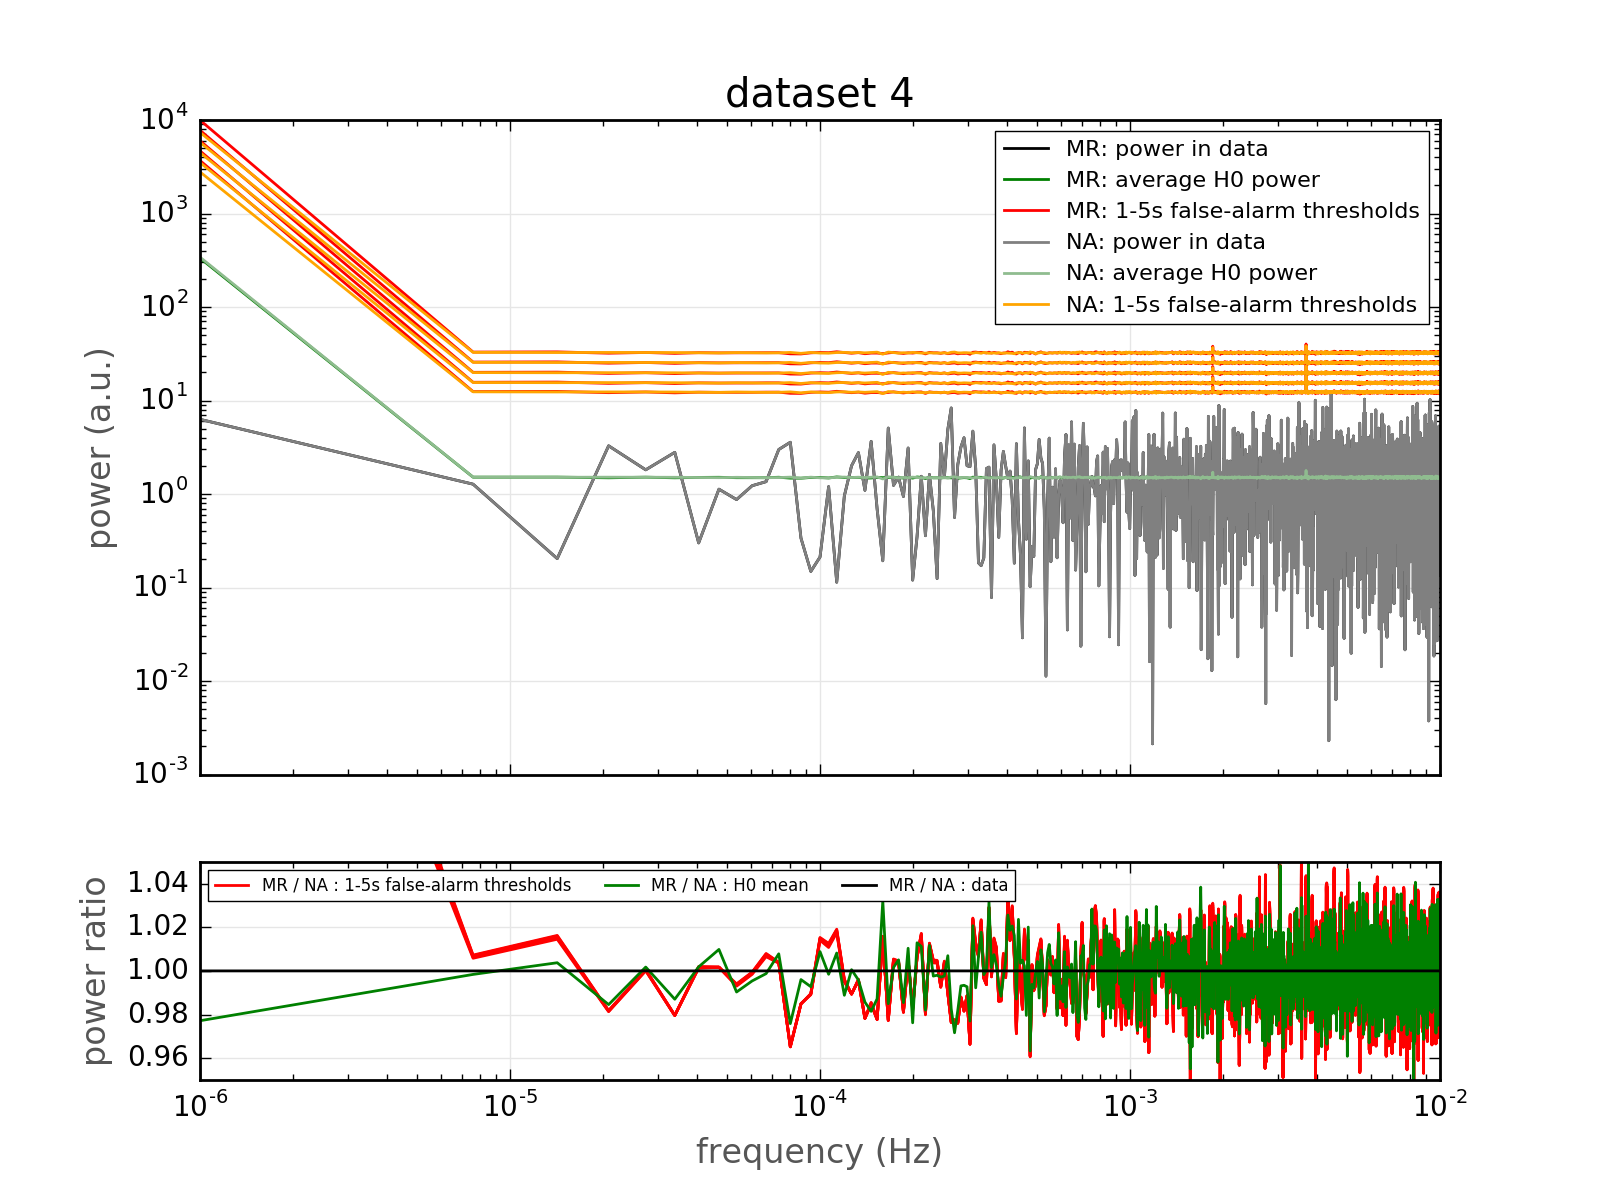
\includegraphics[width=0.32\linewidth]{gfx/axions/comparison/comparison_detection_dataset4.png}
  \centering 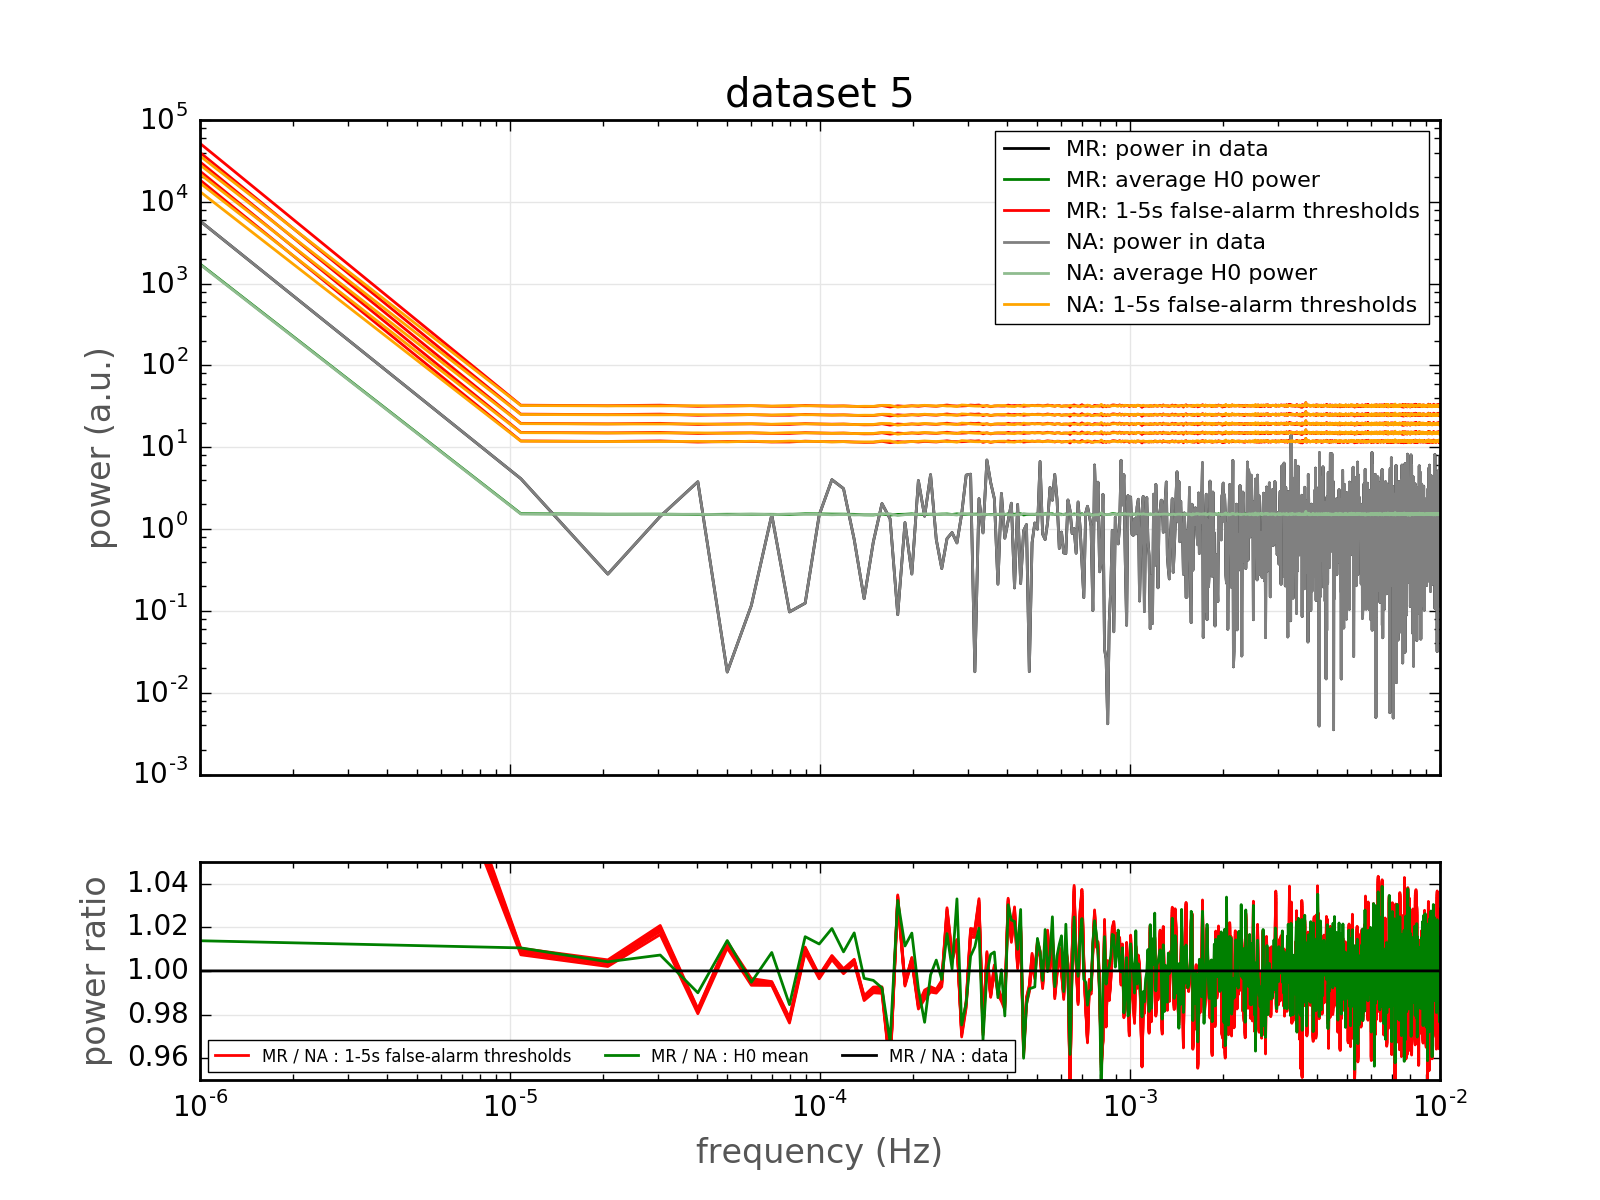
\includegraphics[width=0.32\linewidth]{gfx/axions/comparison/comparison_detection_dataset5.png}
  \centering 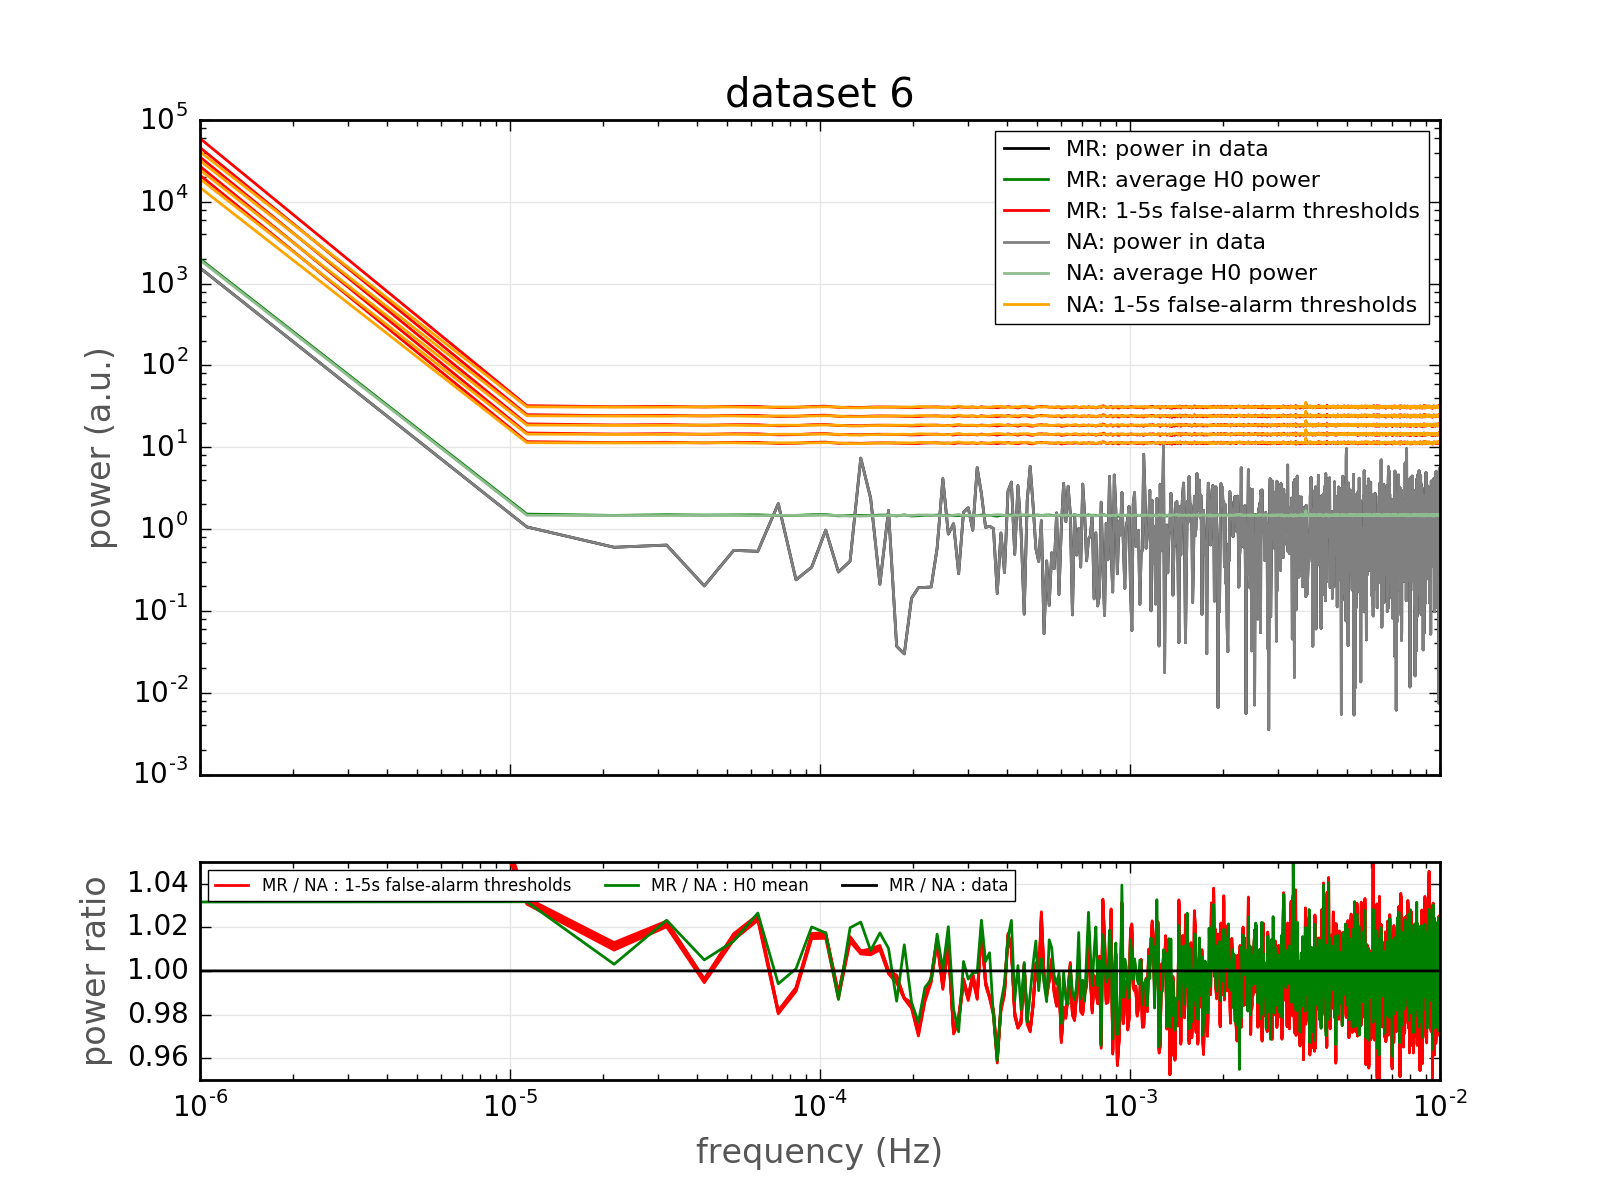
\includegraphics[width=0.32\linewidth]{gfx/axions/comparison/comparison_detection_dataset6.png}
  \centering 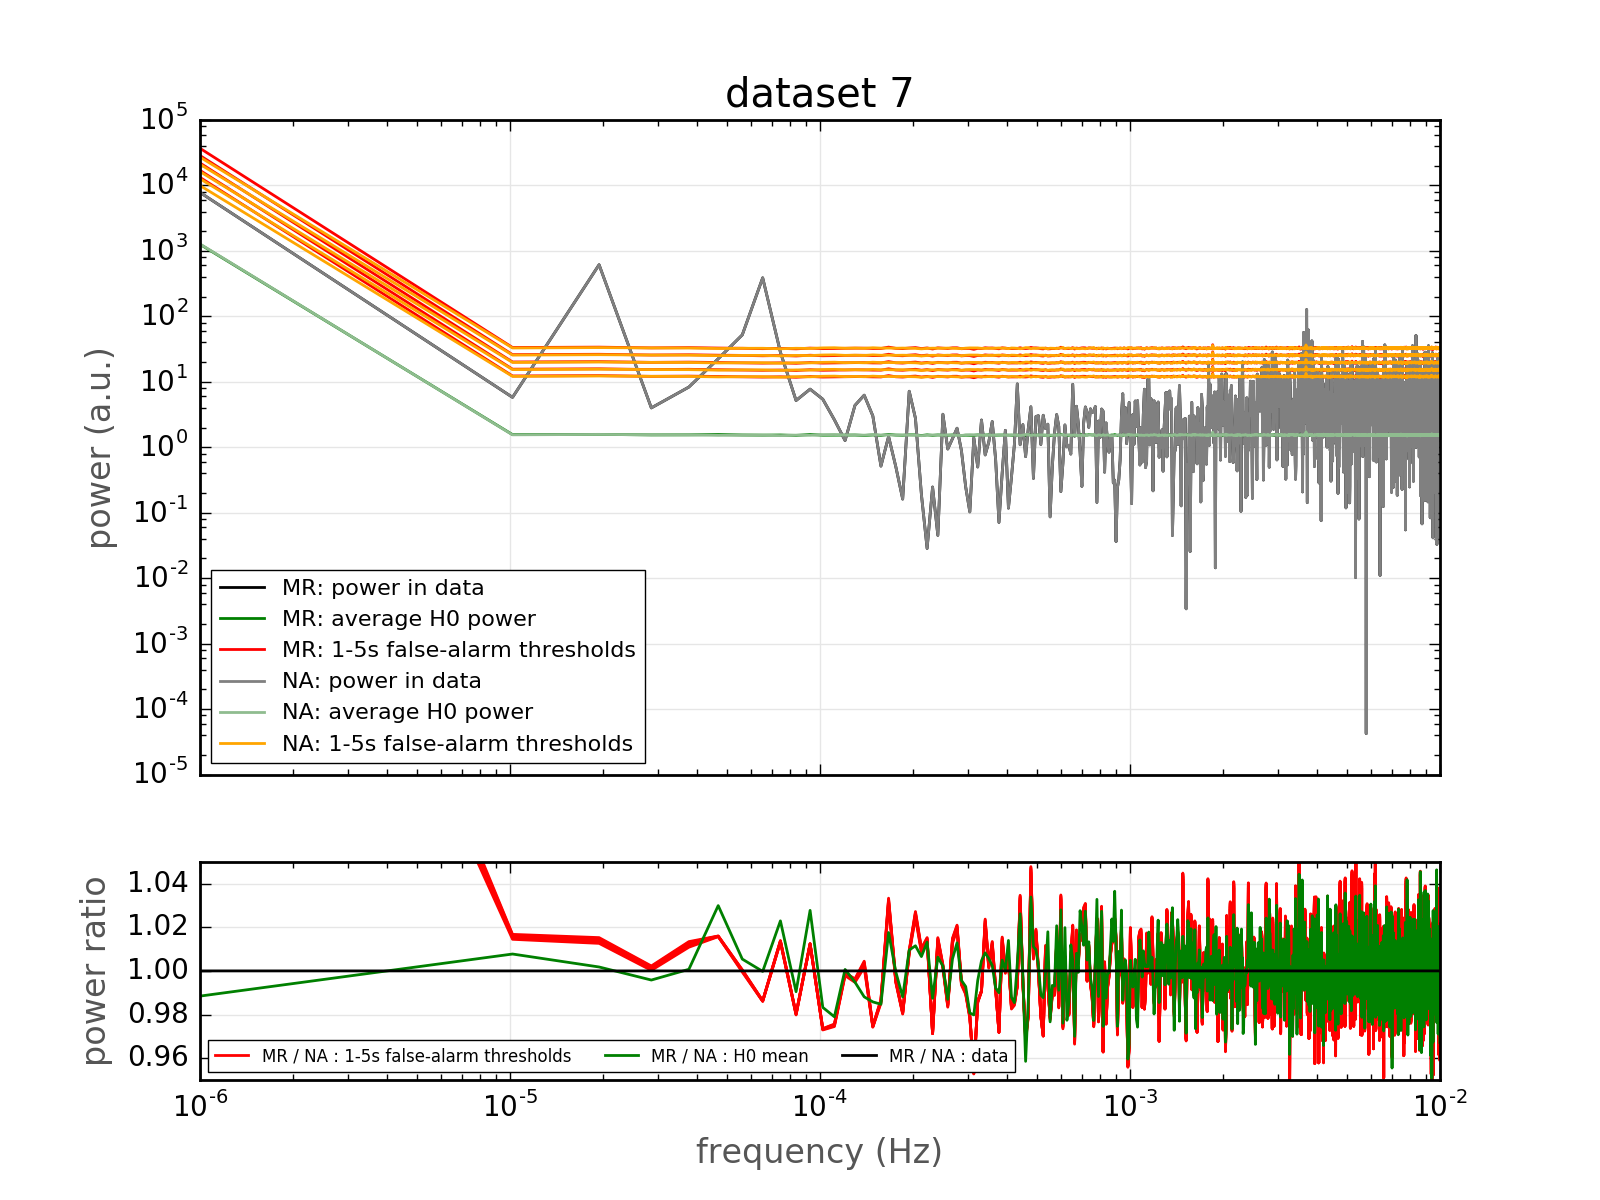
\includegraphics[width=0.32\linewidth]{gfx/axions/comparison/comparison_detection_dataset7.png}
  \centering 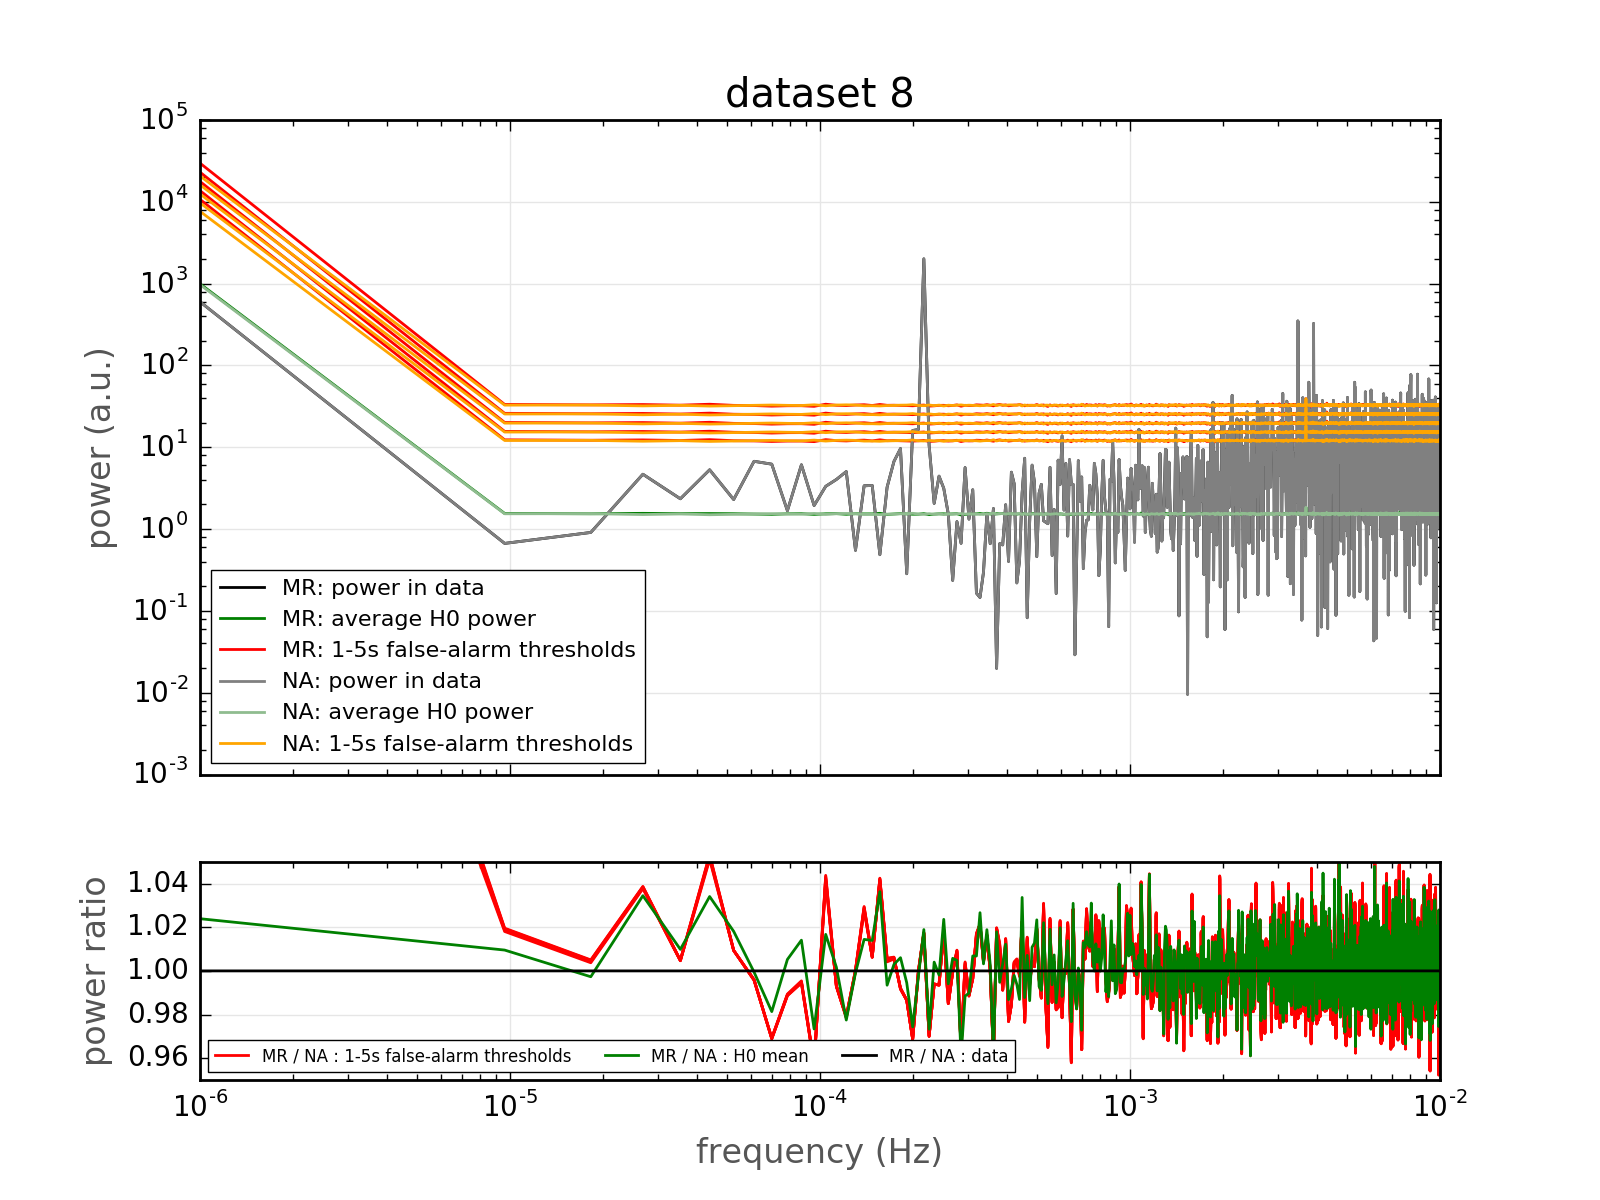
\includegraphics[width=0.32\linewidth]{gfx/axions/comparison/comparison_detection_dataset8.png}
  \centering 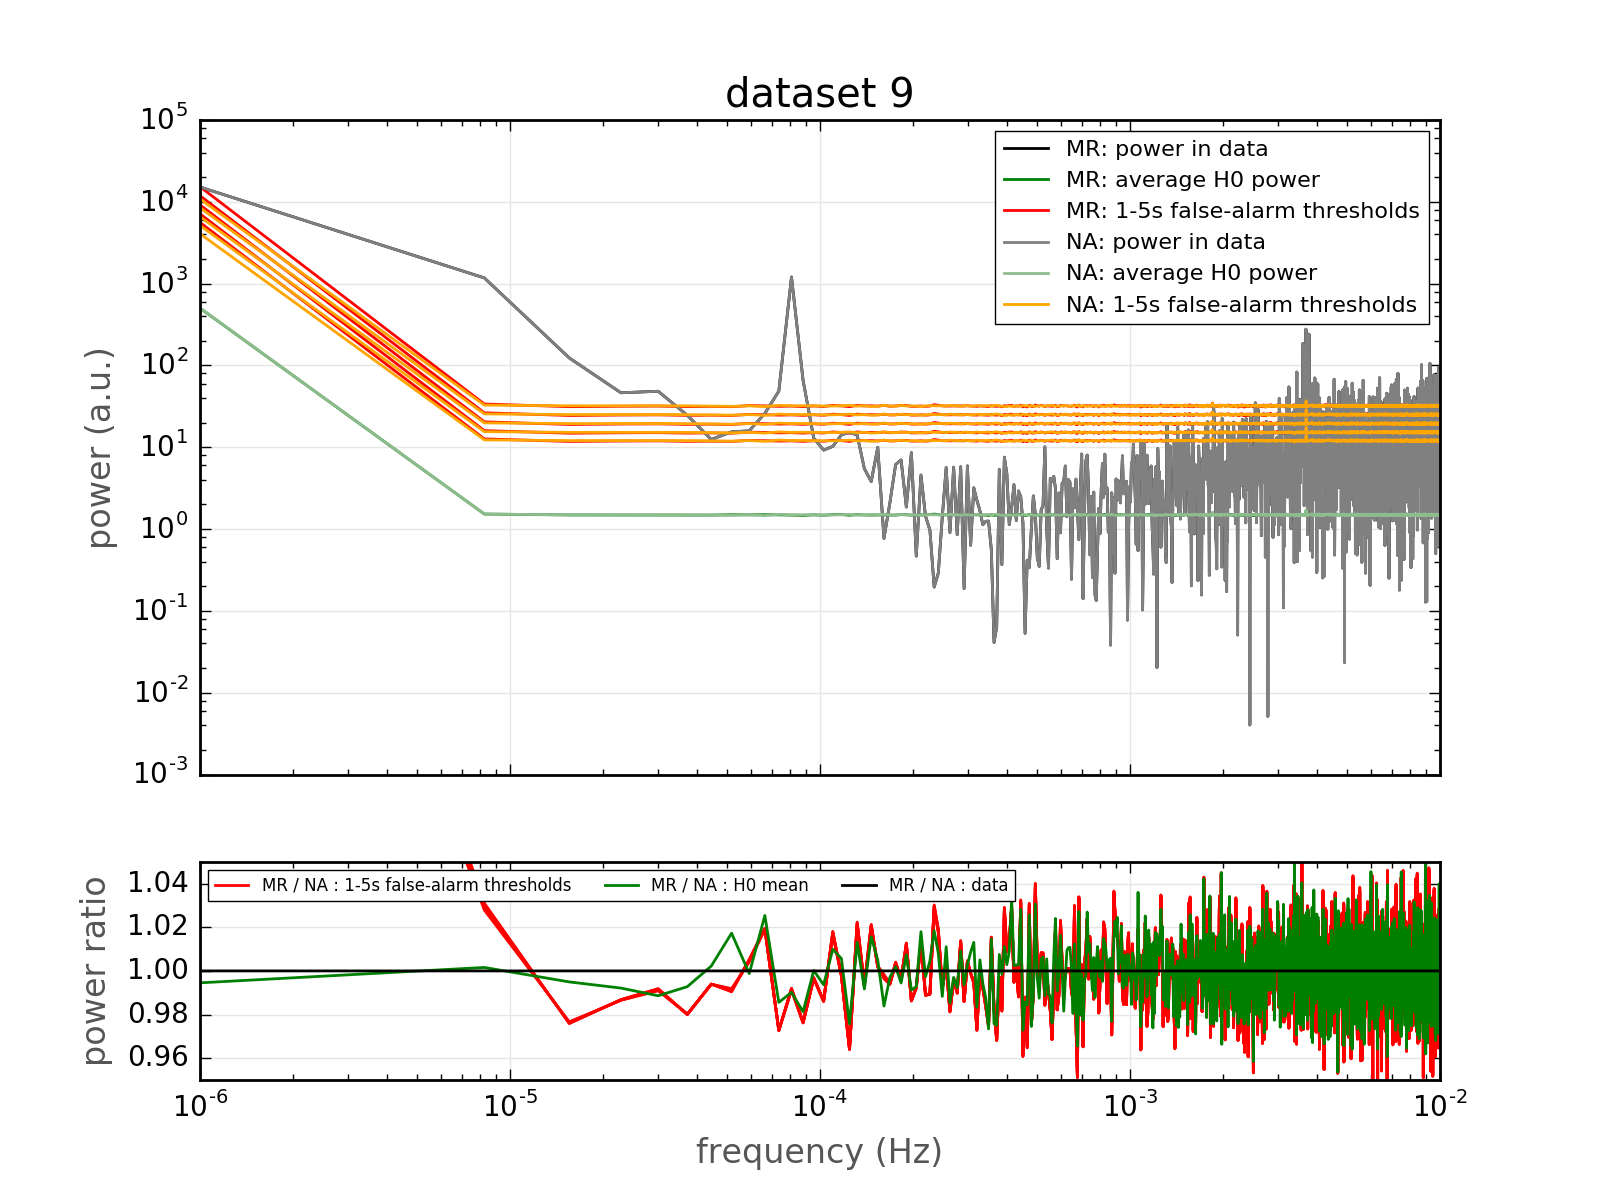
\includegraphics[width=0.32\linewidth]{gfx/axions/comparison/comparison_detection_dataset9.png}
  \caption{Comparison between the analysis implemented by Nicholas Ayres (NA) and Michal  Rawlik (MR). This figure presents the \emph{detection} part of the analysis. Each of the nine plots presents a direct comparison of one fake dataset. For both analyses the following is plotted: (a) the periodogram of the dataset, (b) the average periodogram for the null hypothesis, (c) the 1-,...,5-sigma false alarm thresholds. Below each plot the ratio of the corresponding curves for the two analyses is plotted. For the lowest tested frequency we observe a 40\% difference in the average power for the null hypothesis, as well as the false--alarm thresholds. This single point lies outside the plotted area. For all the other frequencies disagreement is dominated by numerical noise. The periodograms of the datasets agree on the $10^{-6}$ level.}
  \label{fig:comparison_detection}
\end{figure*}

\begin{figure*}[tb]
  \centering 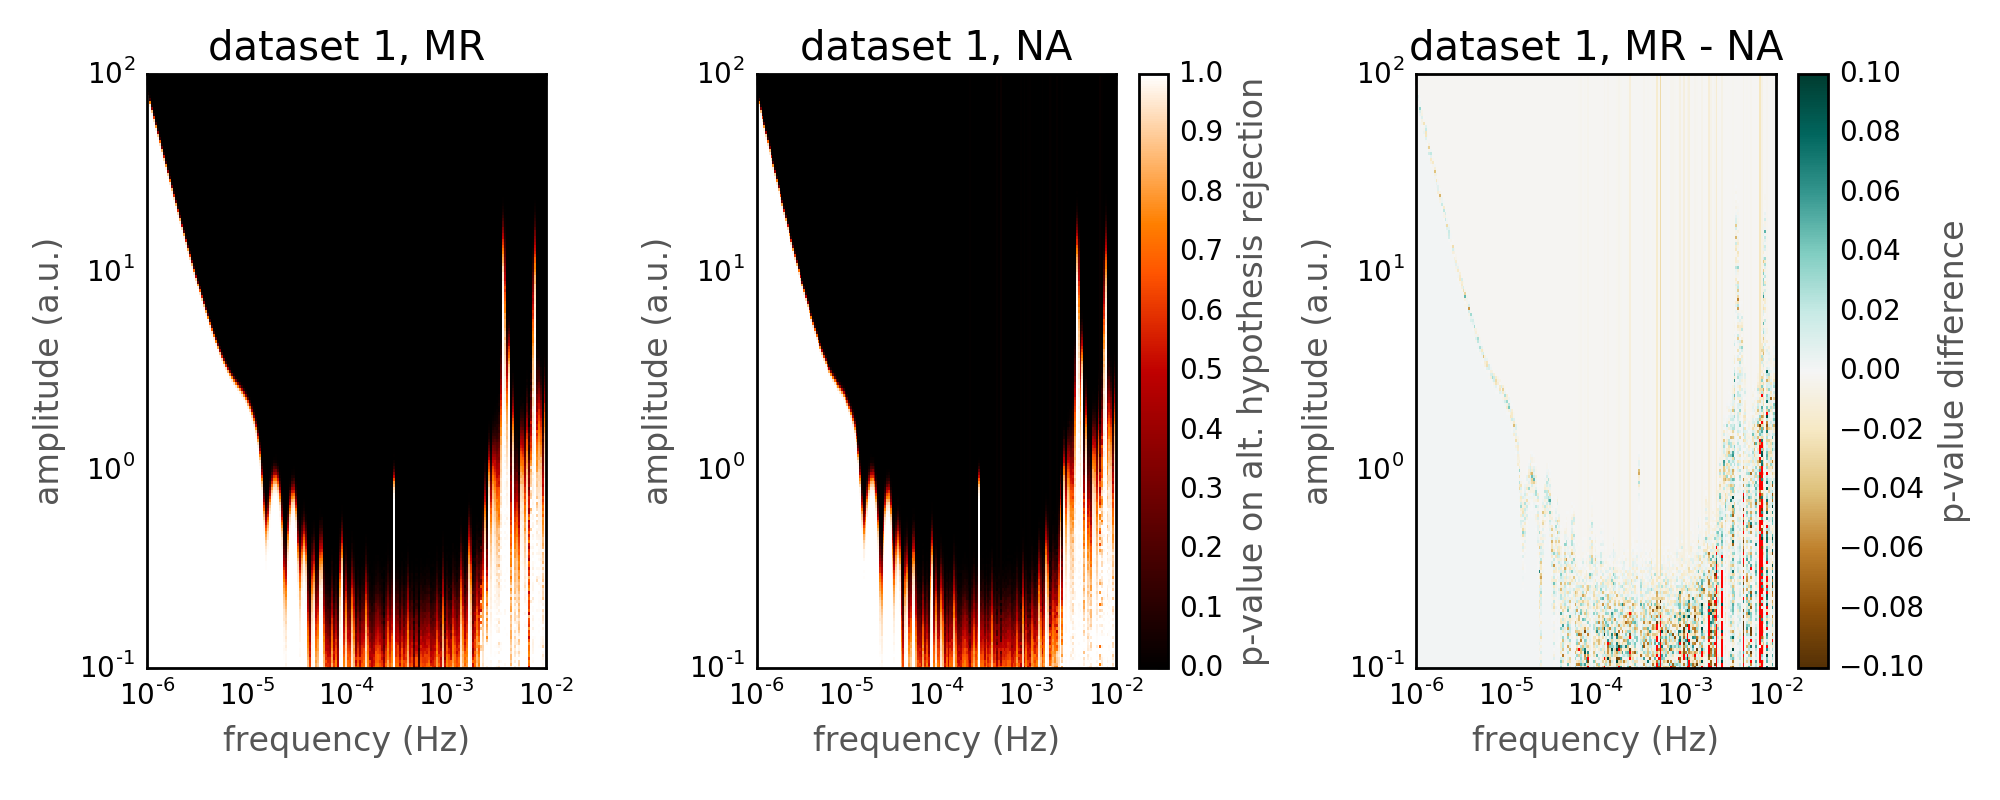
\includegraphics[width=0.45\linewidth]{gfx/axions/comparison/comparison_exclusion_dataset1.png}
  \centering 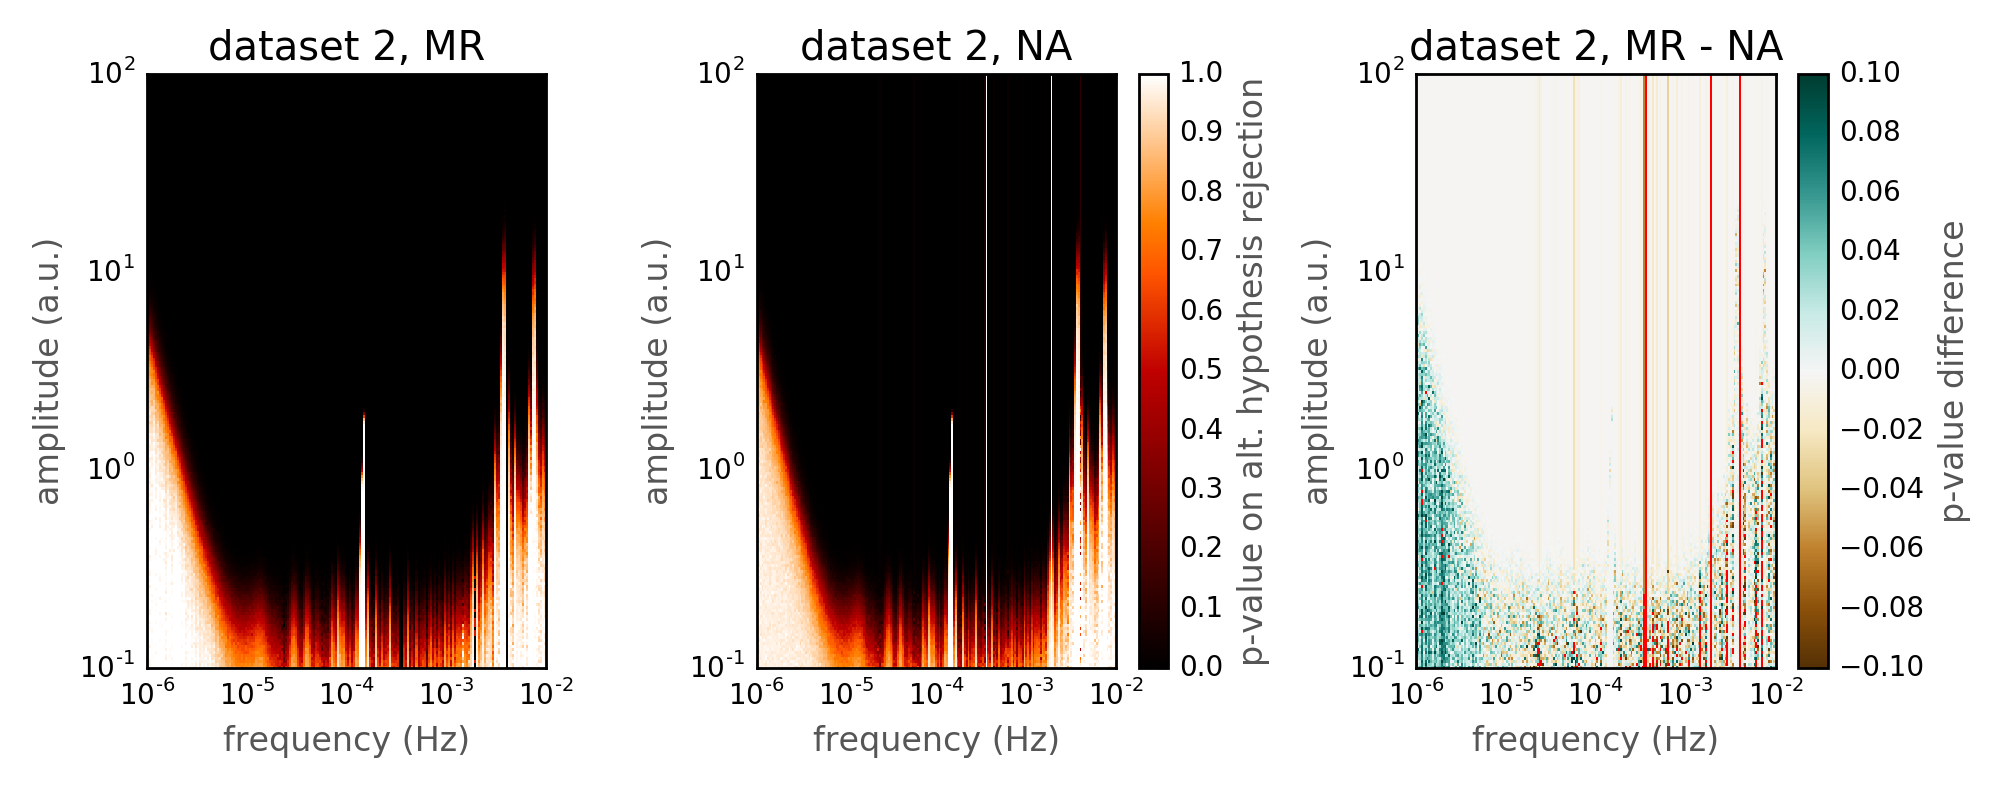
\includegraphics[width=0.45\linewidth]{gfx/axions/comparison/comparison_exclusion_dataset2.png}
  \centering 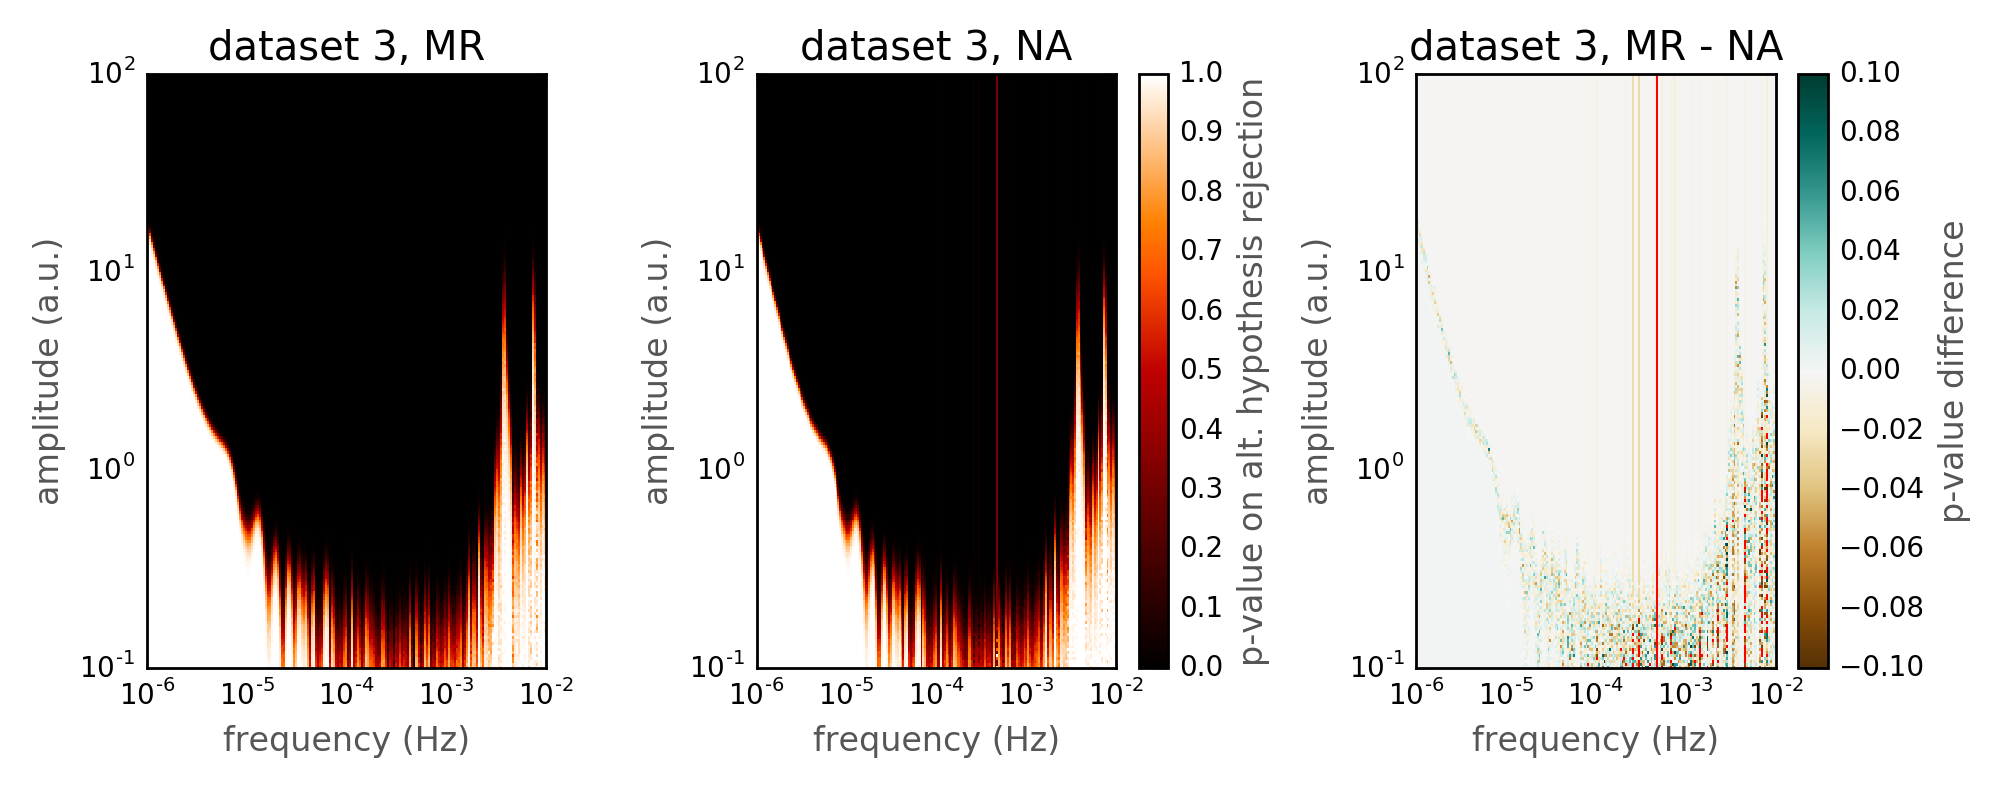
\includegraphics[width=0.45\linewidth]{gfx/axions/comparison/comparison_exclusion_dataset3.png}
  \centering 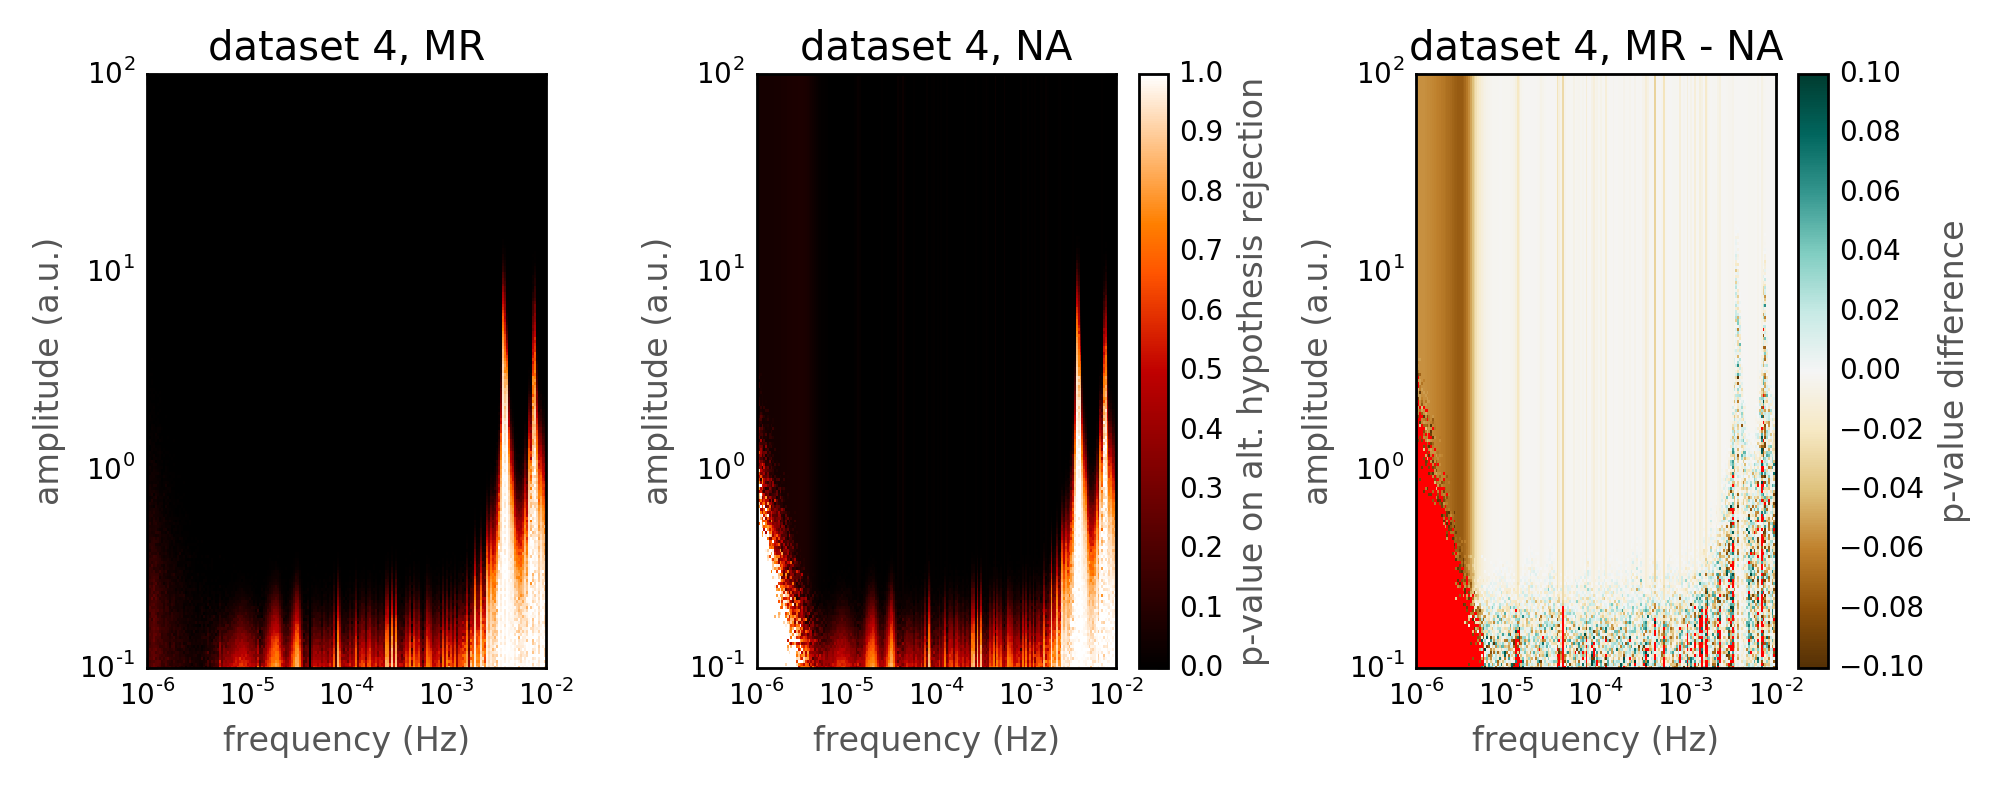
\includegraphics[width=0.45\linewidth]{gfx/axions/comparison/comparison_exclusion_dataset4.png}
  \centering 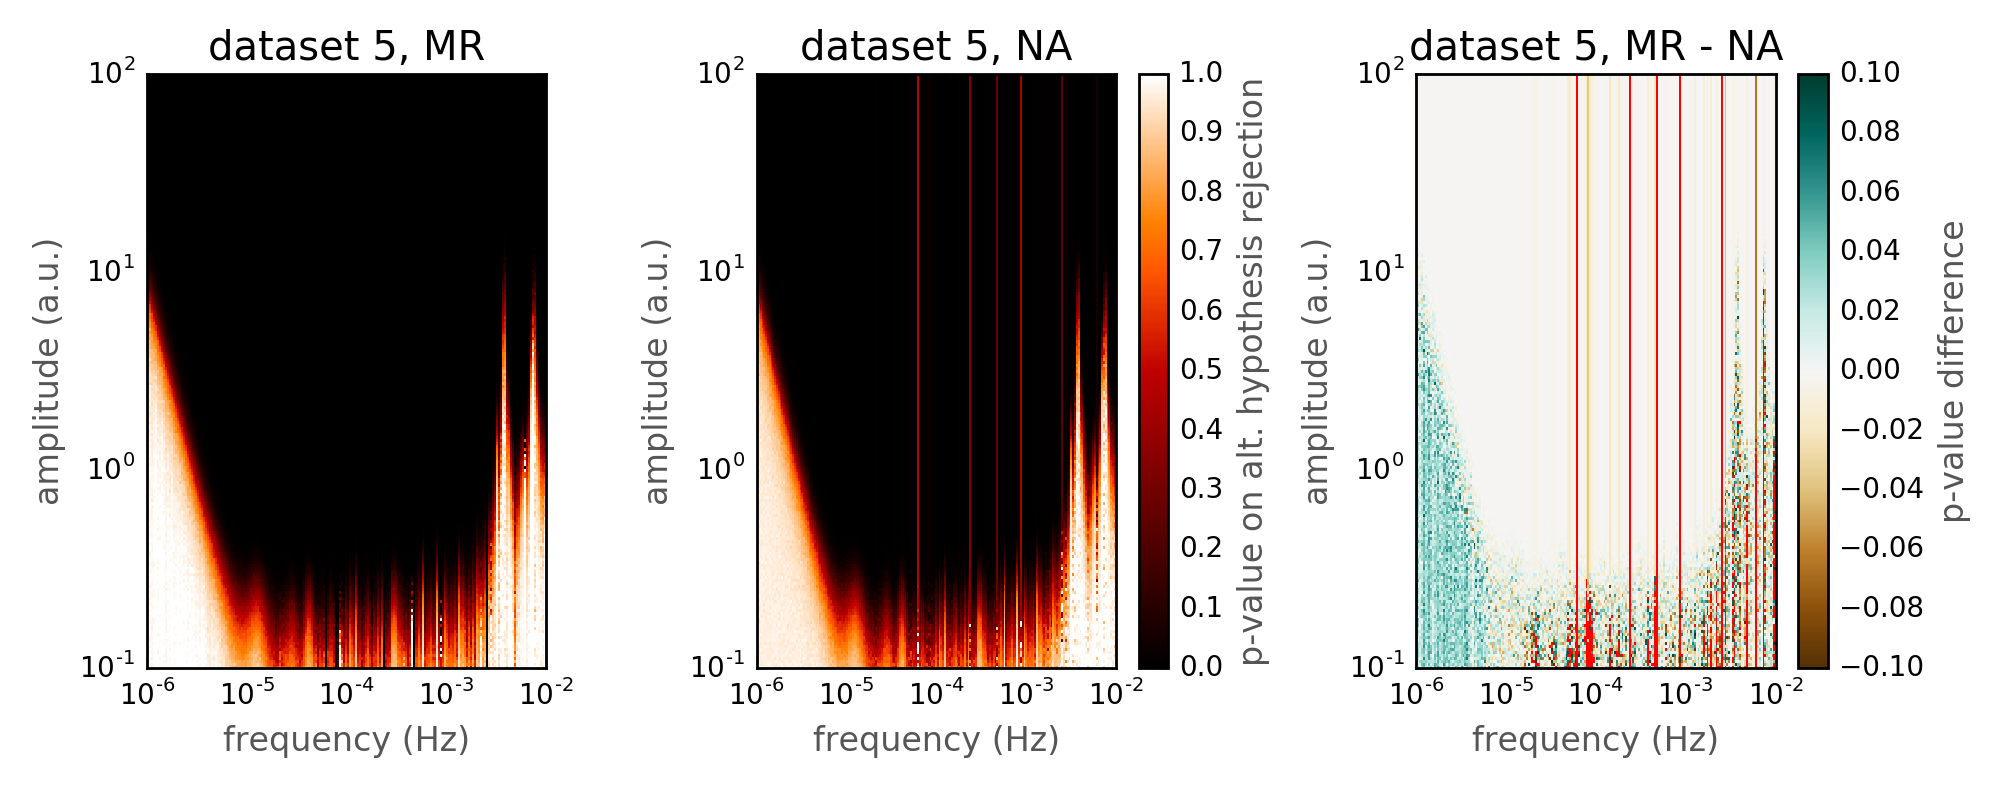
\includegraphics[width=0.45\linewidth]{gfx/axions/comparison/comparison_exclusion_dataset5.png}
  \centering 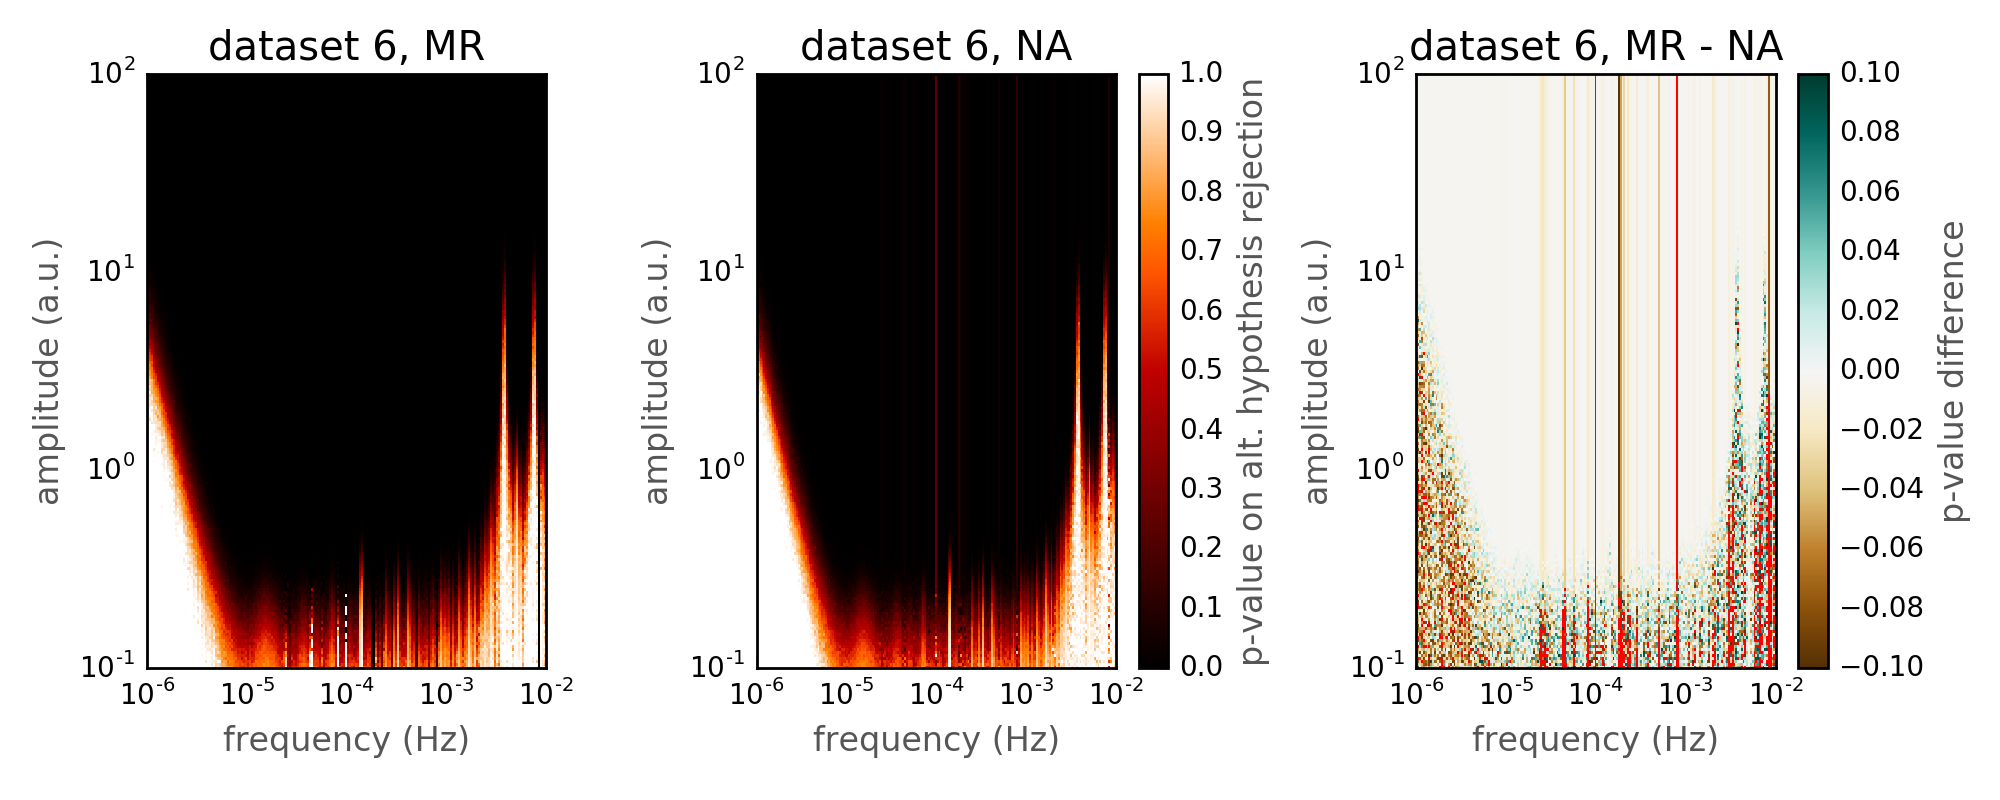
\includegraphics[width=0.45\linewidth]{gfx/axions/comparison/comparison_exclusion_dataset6.png}
  \centering 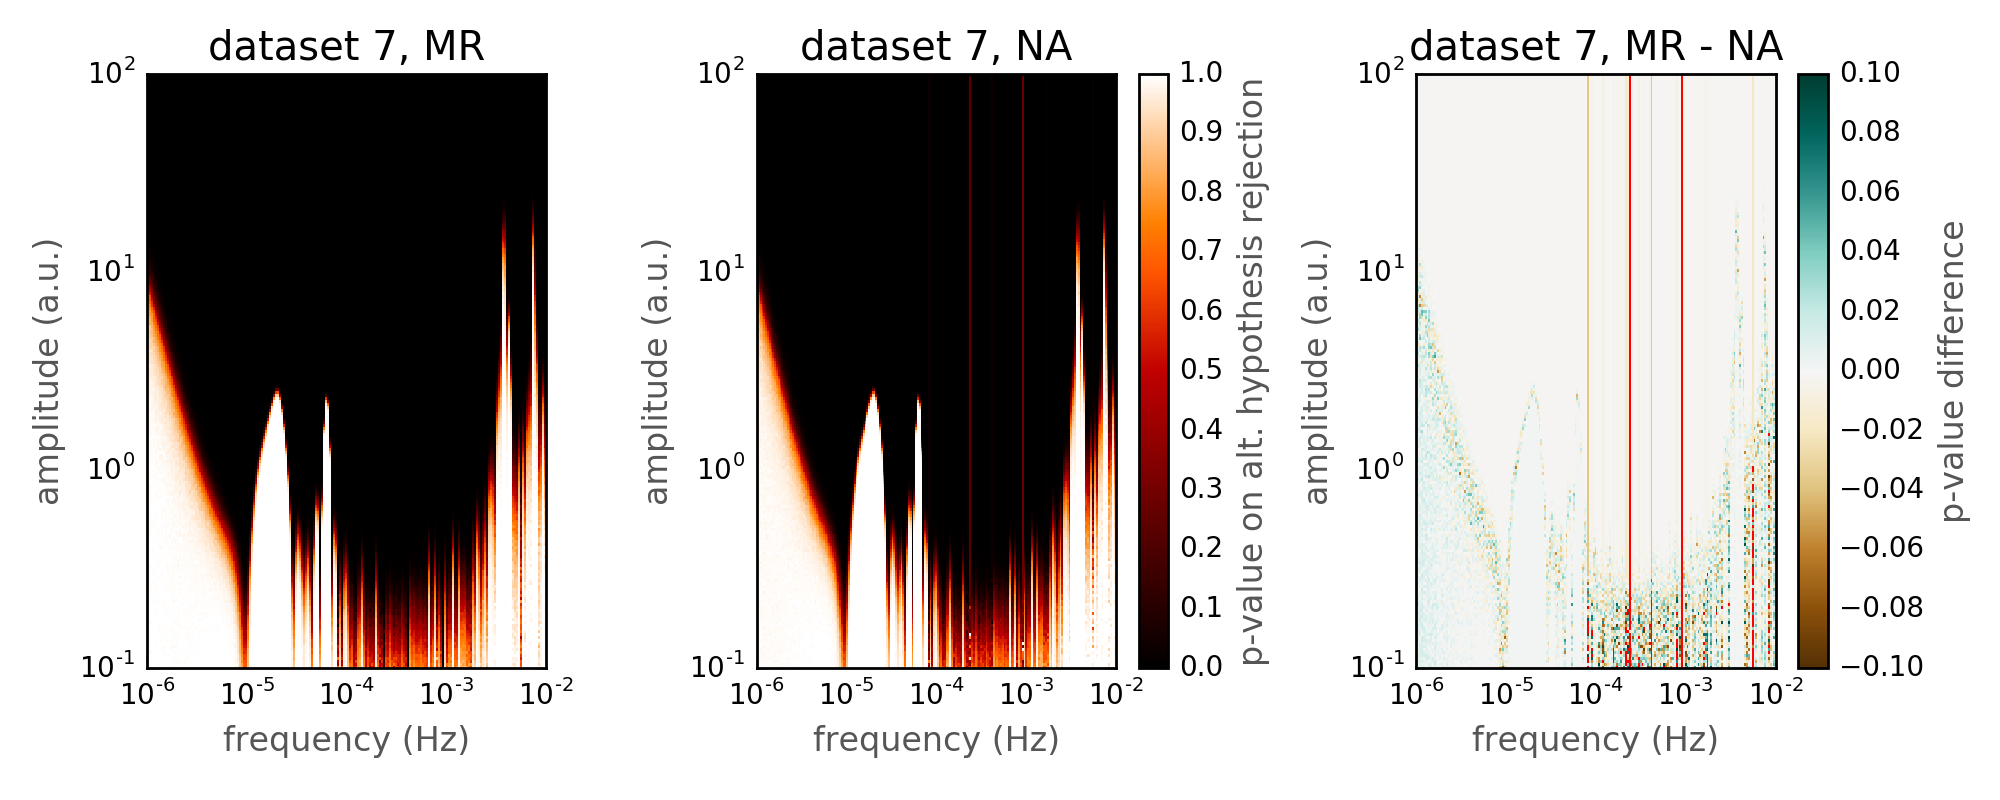
\includegraphics[width=0.45\linewidth]{gfx/axions/comparison/comparison_exclusion_dataset7.png}
  \centering 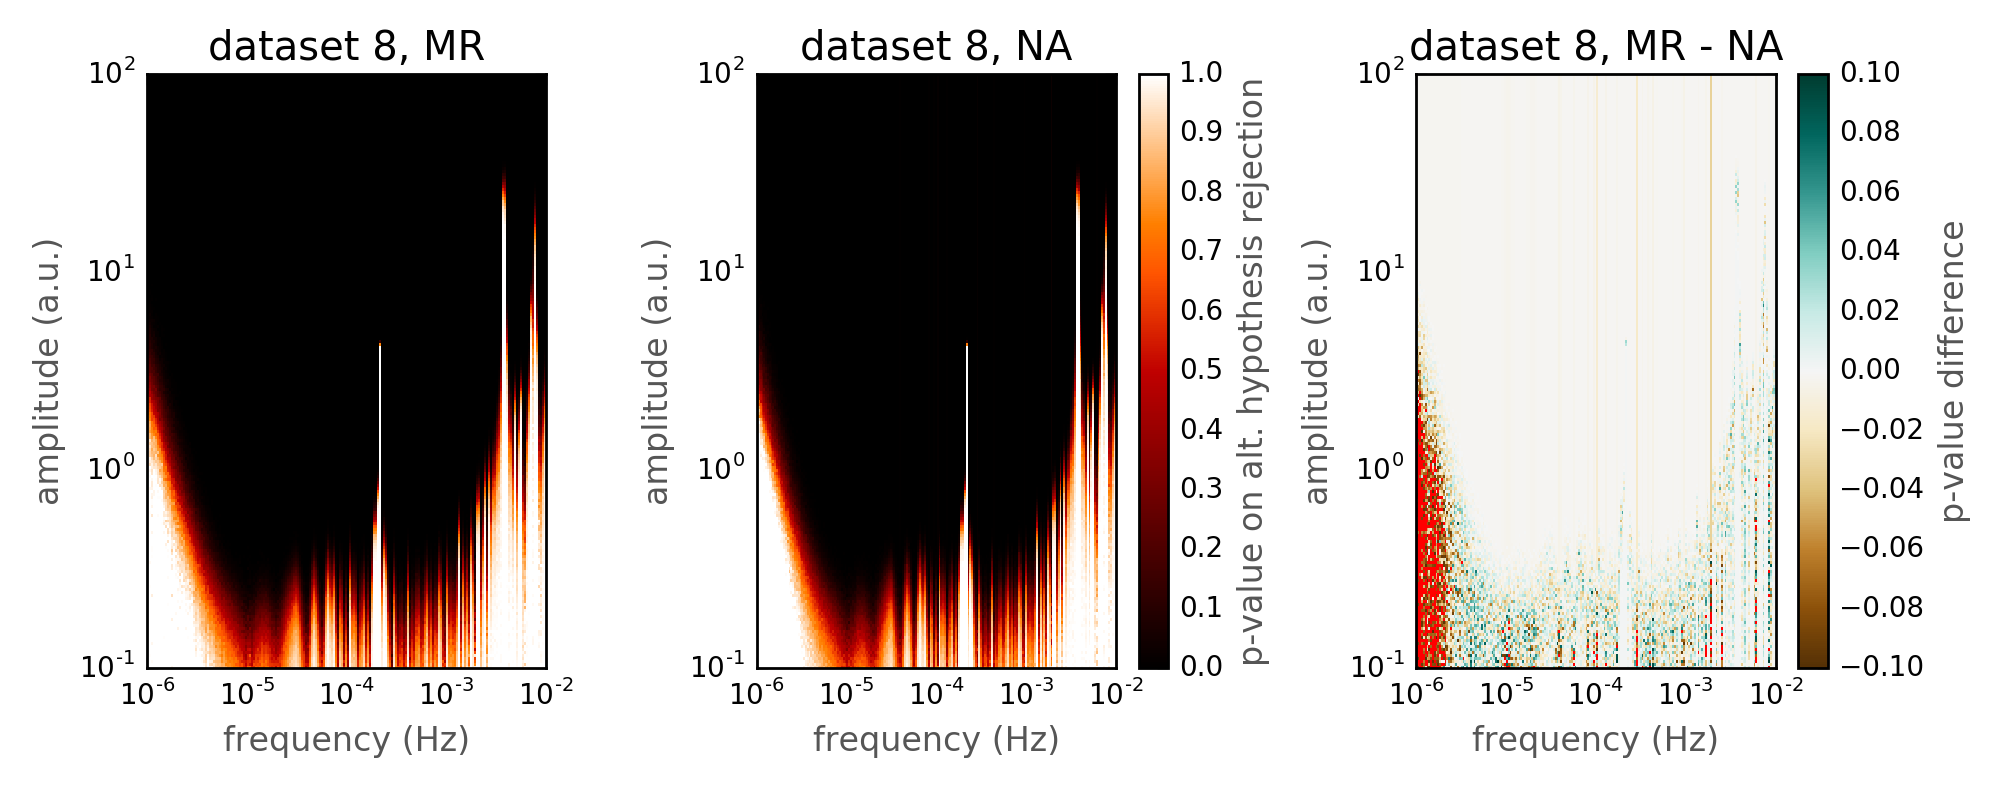
\includegraphics[width=0.45\linewidth]{gfx/axions/comparison/comparison_exclusion_dataset8.png}
  \centering 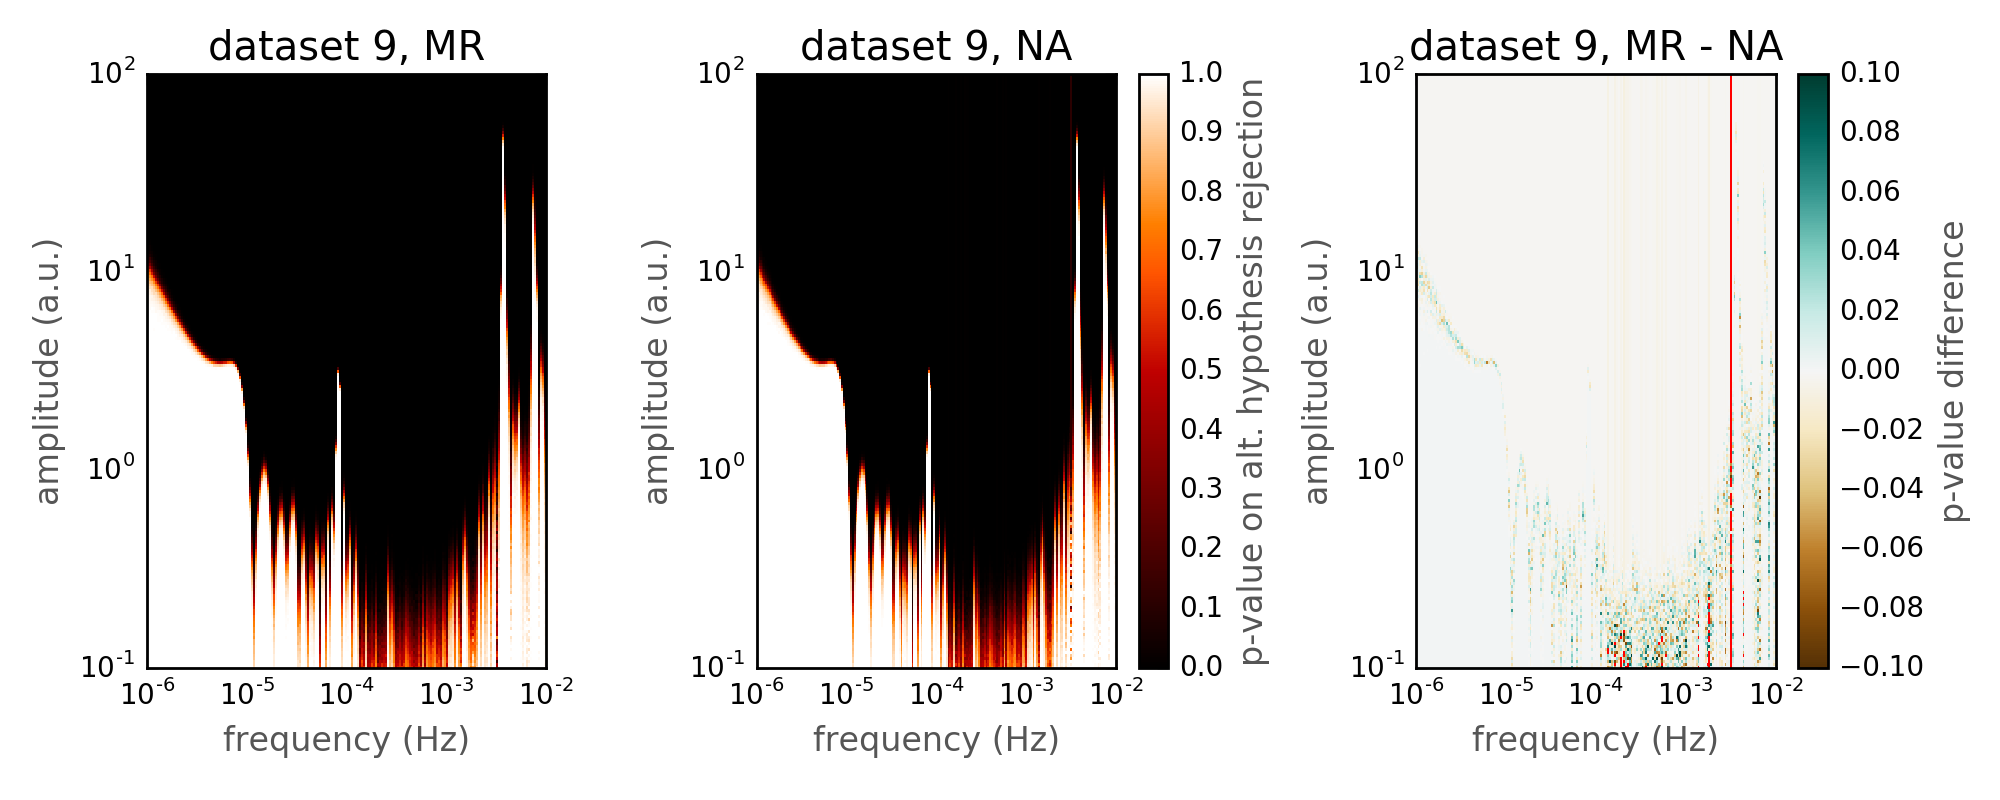
\includegraphics[width=0.45\linewidth]{gfx/axions/comparison/comparison_exclusion_dataset9.png}
  \caption{Comparison between the analysis implemented by Nicholas Ayres (NA) and Michal  Rawlik (MR). This figure presents the \emph{exclusion} part of the analysis. For each fake dataset three maps in the signal parameter space (frequency--amplitude) are shown. From left to right: (a) p--value on exclusion as calculated by Michał Rawlik (MR), (b) p--value on exclusion as calculated by Nicholas Ayres (NA), (c) the difference of the two. Differences larger then 0.1 are marked red.}
  \label{fig:comparison_exclusion}
\end{figure*}

\section{Derivation of what we measure with R}
\label{Sec:R_derivation}

\begin{align}
H &= - \boldsymbol{\mu} \cdot \mathbf{B} - \mathbf{d} \cdot \mathbf{E} \\
h \nu &= 2 \left( \boldsymbol{\mu} \cdot \mathbf{B} \pm \mathbf{d} \cdot \mathbf{E} \right) = 2 \left(\mu B \pm d E \right) \\
R &= \frac{\nu_n}{\nu_{Hg}} = \frac{ \frac{2}{h} \left( \mu_n B + d_n E \right) }{ \frac{2}{h} \left( \mu_{Hg} B + d_{Hg} E \right) } = \nonumber \\
    &= \frac{ \left( \mu_n B \pm d_n E \right) }{ \left( \mu_{Hg} B \pm d_{Hg} E \right) } = \nonumber \\
    &= \frac{ \mu_n B }{ \left( \mu_{Hg} B \pm d_{Hg} E \right) } \pm \frac{ d_n E }{ \left( \mu_{Hg} B \pm d_{Hg} E \right) } = \nonumber \\
    &= \frac{\mu_n}{\mu_{Hg}} \cdot \frac{1}{ 1 \pm \frac{d_{Hg} E}{\mu_{Hg} B}} \pm \frac{d_n E}{\mu_{Hg} B} \cdot \frac{1}{1 \pm \frac{ d_{Hg}E }{ \mu_{Hg} B}} = \nonumber \\
    &= \left\{ \frac{1}{1 \pm x} = 1 \mp x \right\} = \nonumber \\
    &= \frac{\mu_n}{\mu_{Hg}} \mp d_{Hg} \frac{\mu_n}{\mu_{Hg}} \frac{E}{\mu_{Hg} B} \pm d_n \frac{E}{\mu_{Hg} B} \mp d_n d_{Hg} \left( \frac{E}{\mu_{Hg} B} \right)^2 \\
\delta R &\approx \left( d_n \mp  d_{Hg} \frac{\mu_n}{\mu_{Hg}} \right) \frac{E}{\mu_{Hg} B} = \left\{ \boldsymbol{\mu} = \gamma \mathbf{S} \right\} \nonumber \\
   & = \left( d_n \mp  d_{Hg} \frac{\gamma_n}{\gamma_{Hg}} \right) \frac{2 E}{\gamma_{Hg} h B}
\end{align}
